\documentclass{article}
\usepackage{graphicx} 
\usepackage{amssymb}
\usepackage{float}
\usepackage{amsmath}

\title{Econometría Avanzada I}
\author{Milena Poggiese}
\date{April 2024}

\usepackage{amsmath}
\usepackage{amsthm} % Agregar este paquete para usar \newtheorem

\newtheorem{definition}{Definition}[section]
\newtheorem{theorem}{Theorem}[section]
\newtheorem{lemma}{Lemma}[section]


\begin{document}

\maketitle{Ramanathan, 1993}

\section{Basic probability}
\subsection{Sample space, sample points and events}
Starting point of the investigation: an \textbf{experiment}. It is a \textbf{random experiment if it}
\begin{description}
    \item[\textbf{i.} all possible distinct outcomes are known ahead of time]
    \item[\textbf{ii.}the outcome of a particular trial is not known \textit{a priori}]
    \item[\textbf{iii.}the experiment can be duplicated under ideal conditions] 
\end{description}

The totality of all possible oUtcomes of the experiment is referred to as the \textbf{sample space} denoted by \textit{S}. Its distinct individual elements are called \textbf{sample points/elementary events}.
An \textbf{event} is a subset of a sample space and is a set of sample points that represents several possible outcomes of an experiment. The \textbf{impossible event} is denoted by $\emptyset$. A sample space with \textbf{finite} or \textbf{countably infinite} sample points is a \textbf{discrete space}. A \textbf{continuous space} is one with an uncountably infinite number of sample points. 

We can represent the sample spaces using Venn diagrams:

\begin{figure}[h]
    \centering
    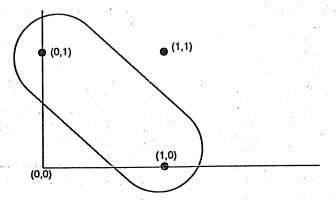
\includegraphics[height=1in]{pics/venn sample space.jpg}
    \caption{Sample space for tossing a coin twice}
\end{figure}

\subsection{Some results from set theory}

\begin{definition}
The \textbf{sample space} is denoted by $S$. \( A \) =  \( S \) implies that the events in \( A \) must always occur.The empty set is a set with no elements and is denoted by $\emptyset$.

The set of all elements not in \( A \) is called the \textbf{complement} of \( A \) and is denoted by \( A^{C} \). \( A^{C} \) occurs if and only if \( A\) doesn't occur.

The set of all points in either a set \(A\) or a set \(B\) ot both is called the \textbf{union} of the two sets and is denoted by \(\cup\). \(A \cup A^C\) = \(S\). Either \(A\) or \(B\) occur in \(A\cup B\).

The set of all elements in both \(A\) and \(B\) is called the \textbf{intersection} of the two sets and is represented by \(\cap\). Both \(A\) and \(B\) occur in \(A\cap B\).

\(A\cap B\)=$\emptyset$ implies than \(A\) and \(B\) cannot occur together: they are \textbf{disjoint} or \textbf{mutually exclusive}.

\(A\subseteq B\) means that \(A\) is contained in \(B\) or that it's a \textbf{subset} of B. Every element of \(A\) is in \(B\).

\end{definition}

\begin{figure}(b)
    \centering
    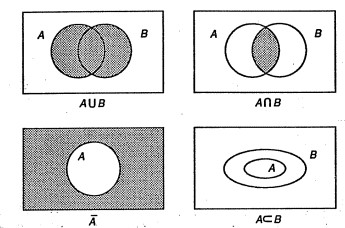
\includegraphics{pics/venn sets.jpg}
    \caption{Venn diagram representation of union, intersection, etc.}
\end{figure}

\subsection{Boolean Algebra}

The set operations of union, intersection and complementation satisfy a number of postulates that are enumerated below.

\begin{description}
    \item[\textbf{1. Identity}.] There exist unique sets $\emptyset$ and \(S\) such that, for every set \(A\), \(A\cup S\) = \(A\) and \(A\cup \emptyset\) = \(A\). 
    \item[\textbf{2. Complementation}.] For each \(A\) we can define a unique set \(A^C\) such that \(A\cap A^C\) = $\emptyset$ and \(A\cup A^C\) = \(S\). 
    \item[\textbf{3. Closure}.] For every pair of sets \(A\) and \(B\), we can define unique sets \(A\cap B\) and \(A \cup B\). 
    \item[\textbf{4. Commutative}.] \(A \cup B\) = \(B \cup A\). \(A \cap B\) = \(B \cap A\)
    \item[\textbf{5. Associative}.] \((A \cup B)\cup C\) = \(A \cup (B\cup C)\). Also, \((A \cap B)\cap C\) = \(A \cap (B\cap C)\)
    \item[\textbf{6. Distributive}.] \(A \cap (B\cup C)\) = \((A \cap B)\cup(A \cap C)\)
\end{description}
\begin{figure}[h]
    \centering
    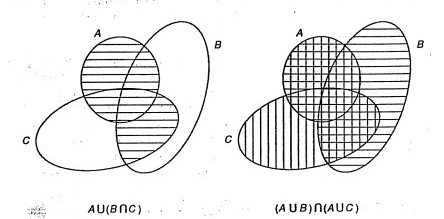
\includegraphics{pics/distributive .jpg}
    \caption{Distributive property of sets}
\end{figure}


\textbf{De Morgan's Laws:}
\begin{description}
   \item[(a)] \( (A \cup B)^\mathsf{C} \) = \(A^C \cup B^C\). The complement of a union is the intersection of the complements.
   \item[(b)] \((A \cap B)^\mathsf{C} \) = \(A^C \cup B^C\). The complement of an intersection is the union of the complements.
\end{description}
Proof with Venn diagrams (trabajo práctico)

\subsection{Borel Fields and $\sigma$-fields}

It is clear from the operations on sets that by combining sets we obtain other sets. In order to make sure that the result of combining events is always an event, we have to \textbf{impose some mathematical structure} to it: \( \mathcal{F}\) or field. Otherwise, attribution of probabilities to events may sometimes not make sense. Sets which have the required structure are $\sigma$-fields or $\sigma$-algebras associated with \(S\).

\begin{definition}
    Let \( \mathcal{F}\) be a nonempty set of subsets of \(S\) that is also nonempty. \( \mathcal{F}\) is said to be a $\sigma$-field if the following two conditions hold:
    \begin{description}
        \item[(1)] if \(A \in \mathcal{F}\), then \(A^C \in \mathcal{F}\). \textbf{Closure under complementation}
        \item[(2)] if \(A_i \in \mathcal{F}\) for i=1,2,..., then \(\bigcup_{i=1}^{i=\infty} A_i \in \mathcal{F}\). \textbf{Closure under countable unions}
    \end{description}
\end{definition}

\begin{theorem}
    Definition 1.2 implies the following: 
    \begin{description}
        \item[(1)] \(S\in \mathcal{F}\),
        \item[(2)] \(\emptyset\in \mathcal{F}\) 
        \item[(3)] if \(A_i\in \mathcal{F}\) for i=1,2,.., then \(\bigcap_{i=1}^{i=\infty}A_i \in \mathcal{F}\).
    \end{description}  
\end{theorem}

\textbf{Proof}: the first property follows from the fact that \(A\) and \(A^C\) being in \( \mathcal{F}\) implies that \(S\)= \(A \cup A^C \) is also in \( \mathcal{F}\). Also, \( \emptyset\) = \(S^C \in \mathcal{F}\). 

Part 3 of the Theorem is given by DeMorgan's law:
\begin{equation*}
    \bigcap_{i=1}^{i_{\infty}} A_i = \left( \bigcup_{i=1}^{\infty} A_i^C \right)^C
\end{equation*}

which, by definition 1.2, is a member of \( \mathcal{F}\).

It follows from the above that a $\sigma$-field is a \textbf{set of subsets of \(S\) that is closed under complementation, countable unions and countable intersections.} 

\subsection{Borel Fields}

Consider the set \(A_x\)= $\{z:z \leq x\}$ = $\{(-\infty, x]\}$. The complementary set is \(A_x^C\) = $\{z : z \in \mathbb{R} \text{ and } z > x\}$. For different values of $x$, \(A_x\) and \(A_x^C\) constitutes a family of sets called \textbf{Borel sets}. Starting from \(A_x\), if we take countable unions and intersections of \(A_x\) and \(A_x^C\), we can obtain a $\sigma$-field on $\mathbb{R}$. Such a $\sigma$-field is called a \textbf{Borel field} $(\mathcal{B})$.

\subsection{Measurable Spaces}

We often want to have numerically quantifiable measures as otherwise summary characteristics are impossible to obtain. We can define a set function $\mu$\((A)\) that is simply the number of elements in \(A\) is the number is finite and $\ + \infty$ otherwise. This is a \textbf{counting measure}. A \textbf{measure} is a nonnegative countably additive set function $\mu$ defined on $\mathcal{F}$ that has the following properties:
\begin{description}
    \item[(1)] $\mu(A) \geq \mu(\emptyset) = 0$ for all $A \in \mathcal{F}$
    \item[(2)] if \(A_i \in \mathcal{F}\) are disjoint sets, then $ \mu (\bigcup_{1}^{n} A_i) = \sum_i \mu (A_i) $
\end{description}

Thus, $ \mu : \mathcal{F} \rightarrow \mathbb{R} $. A probability measure is one that has the property $\mu (S)$ = 1.

The pair $ (S, \mathcal{F})$ is a \textbf{measurable space}, a space on which a measure can be assigned.

\subsection{Probability}

\begin{definition}. 
Axiomatic definition

The \textbf{probability} of an event \(A \in \mathcal{F}\) is a real number such that:
    \begin{enumerate}
        \item [1.] $P(A) \geq 0$ for every \(A \in \mathcal{F}\)
        \item [2.] the probability of an entire sample space \(S\) is 1; P (\(S\))=1, and
        \item[3.] if \(A_1\), \(A_2\), ..., \(A_n\) are mutually exclusive events, then \( P(A_1 \cup A_2 \cup ... \cup A_n) = \sum_i P(A_i) \)
    \end{enumerate}
The triple \((S, \mathcal{F}, P)\) is referred to as the \textbf{probability space} and P is a \textbf{probability measure}.
   
\end{definition}

\begin{definition}
Classical definition
    
If an experiment has \( n \) (\( n < \infty \)) mutually exclusive and equally likely outcomes, and if \( n_A \) of these outcomes have an attribute A (that is, the event A occurs in $n_A$ possible ways), then the probability of A is \( \frac{n_A}{n} \), denoted as \( P(A) = \frac{n_A}{n} \).
\end{definition}

\begin{definition}
Frequency definition
Let $n_A$ be the number of times the event A occurs in n trials on an experiment. If there exists a real number p such that \( p = \lim_{n \to \infty} \frac{n_a}{n} \), then p is called the probability of A and is denoted as P(A).
\end{definition}

Thus the probability of an event is its limiting frequency when an experiment is repeated indefinitely. The usefulness of this definition is, therefore, when the number of observations is large.
 \begin{figure} [h]
     \centering
     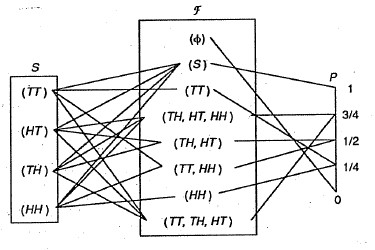
\includegraphics{pics/probability space.jpg}
     \caption{Graphic representation of a probability space (two tosses of heads and tails}
     \label{fig:enter-label54}
 \end{figure}

\subsubsection{Subjective Probability}

Example of subjective or personal probability: the odds are 2 to 1 that candidate X will be elected. It's based in \textbf{educated guesses} or intuition. In statistical inference, the practicality of this approach stems from using prior beliefs or new information in updating previous model specifications.

The axiomatic definition of probability enables us to derive a number of properties of probabilities:

\begin{theorem}
    \( P(A^C)=1-P(A)\)
\end{theorem}

\textbf{Proof:} \(A \cup A^C = S \text{ and } A \cap A^C = \emptyset\). By the second and third axioms, \(P(A) + P(A^C)=1\). Therefore, \(P(A^C)=1-P(A)\)

\begin{theorem}
    \(P(A) \leq 1\)
\end{theorem}

\textbf{Proof:} \(P(A^C) \geq 0\) by the first axiom. From this and Theorem 2, \(P(A) \leq 1\).

\begin{theorem}
    \(P(\emptyset)=0\)
\end{theorem}

\textbf{Proof:} \(S^C=\emptyset. P(S \cup \emptyset)= 1 = P(S)+P(\emptyset). \text{ By Axiom 2,}  P(S)=1. \text{Hence, } P(\emptyset)=0\)

\begin{theorem}
    If \(A \subset B\), then \(P(A) \leq P(B)\)
\end{theorem}

\textbf{Proof:} If \(A \subset B\), then \(B\) can be expressed as \(B = A \cup (A^C \cap B)\) which are disjoint. Hence, \(P(B)=P(A)+P(A^C \cap B) \geq P(A)\) because \(P(A^C \cap B)\).

\begin{theorem}
    \(P(A \cup B) = P(A) + P(B) - P(A \cap B)\)
\end{theorem}

\textbf{Proof:} The set B can be partitioned as \(B = (A \cap B) \cup (A^C \cap B)\) and therefore \(P(B) = P(A \cap B) + P(A^C \cap B)\). Hence \(P(A^C \cap B) = P(B) - P(A \cap B)\). The set \(A \cup B\) can be partitioned as \(A \cup B = A \cup (A^C \cap B)\). Therefore \(P(A \cup B) = P(A) + P(A^C \cap B)\). It then follows that \(P(A \cup B) = P(A) + P(B) - P(A \cap B)\).

\subsubsection{Conditional Probability}
We may want to calculate the probabilities of events when it is known that another event has occurred.
\begin{definition}
    Let A and B be two events in a probability space \((S, \mathcal{F}, P)\) such that \(P(B) > 0\). The \textbf{conditional probability} of A given that B has occurred, denoted by \(P(A|B)\), is given by \(P(A \cap B)/P(B)\)
\end{definition}
Thus, we are looking at the subspace in which the event \(B\) has already occurred. By dividing by \(P(B)\), we are normalizing the probability values so that they add up to 1 in the subspace. The original probability space remains unchanged \textit{even though we are focusing on the subspace which is} \((S, \mathcal{F}, P( . |B))\)

\begin{theorem}{Bayes Theorem}

    If \(A\) and \(B\) are two events with positive probabilities, then
    \begin{equation*}
        P(A|B)= \frac{P(A) P(B|A)}{P(B)}
    \end{equation*}
\end{theorem}
\textbf{Proof:} The proof follows from the definition of conditional probability.

\(P(A|B)= \frac{P(A \cap B)}{P(B)}\)

\(P(A \cap B) = P(B|A) P(A)\)

Combining two equations, we have the desired result.

Example: \(A\) might be a possible strategy of the management and \(B\) a strategy of the union. We might want to infer the probability of occurrence of the preceding event, namely, that the company would adopt \(A\) \textit{knowing the probability of \(B\) given than \(A\) has occurred}. Thus, we might be interested in a \textbf{Bayesian updating} of \(A\). A more common approach is when there are several possible states of nature associated with different probabilities. The following theorem gives the rule for updating probabilities.

\begin{theorem}{Extended Bayes Theorem}

    If \(A_1, A_2, ..., A_n\) constitute a partition of the sample space, so that \(A_i \cap A_j = \emptyset\) for \(i \neq j\) and \(\bigcup_{i} A_i = S\), and \(P(A_i) \neq 0\) for any i, then for a given event \(B\) with \(P(B) > 0\),
    \begin{equation*}
        P(A_i|B)=\frac{P(A_i) P(B|A_i)}{\sum_{i} P(A_i) P(B|A_i)}
    \end{equation*}
\end{theorem}
\textbf{Proof:} By the previous theorem, 
\begin{equation*}
     P(A_i|B)= \frac{P(A_i) P(B|A_i)}{P(B)}
\end{equation*}
Because \(A_i\)'s constitute a partition of \(S\), \(B\) can be written as \(B= \bigcup_{i}(B \cap A_i)\) where each is disjoint from the others. Hence \(P(B) = \sum_{i} P(B \cap A_i) = \sum_{i} P(A_i) P(B|A_i)\). Substitution of this in the above expression establishes the theorem.

\subsection{Statistical Independence}
If the conditional probability of \(A\) given \(B\) is the same as the unconditional probability of \(A\) (\(P(A|B)=P(A)\)), then in assessing the probability of \(A\) there is no informational content in the knowledge that \(B\) has occurred. Thus, the events \(A\) and \(B\) are independent.
\begin{definition}
    Two events \(A\) and \(B\) with positive probabilities are said to be statistically independent if and only if \(P(A|B)=P(A)\). Equivalently, \(P(B|A)=P(B)\) and \(P(A \cap B) = P(A).P(B)\)
\end{definition}
In the case of statistical independence the joint probability of two events is equal to the product of the individual probabilities and, conversely, if the joint probability is the product of individual probabilities, then the events are independent.

\textbf{Statistically independent $\neq$ Mutually exclusive}. If \(A\) and \(B\) are mutually exclusive, then \(A \cap B = \emptyset\) and hence \(P(A \cap B)=0\). But independence requires that \(P(A \cap B\) be the product of the individual \textit{non-zero} probabilities.

\subsection{Sequences and Limiting Sets of Events}
We often encounter sequences of sets of events. For instance, consider the set \(A_n = [x-n,x+n]\) for a fixed \(x\). For different values of \(n\) this defines a sequence of sets. What happens when the number of trials becomes indefinitely large? 
\begin{definition}
    A sequence of sets \(A_1, A_2, A_3, ...\) is called \textbf{monotone increasing} if \(A_1 \subset A_2 \subset A_3 \subset ...\) and \textbf{monotone decreasing} if \(A_1 \supset A_2 \supset A_3 \supset ...\). The limit set is defines as follows:
    \begin{equation*}
        \text{\textit{Monotone increasing: }} \lim_{n \rightarrow \infty} A_n = \bigcup_{i}^{\infty} A_n
    \end{equation*}
    \begin{equation*}
        \text{\textit{Monotone decreasing: }} \lim_{n \rightarrow \infty} A_n = \bigcap_{i}^{\infty} A_n
    \end{equation*}
\end{definition}
\begin{figure} [h]
    \centering
    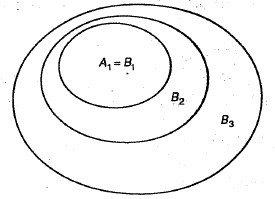
\includegraphics{pics/monotone sets.jpg}
    \caption{Monotone increasing sets}
\end{figure}
\begin{theorem}
    If \(A_1, A_2, ..., A_n, ...\) is a monotone sequence, then
    \begin{equation*}
        P(\lim_{n \rightarrow \infty} A_n)= \lim_{n \rightarrow \infty} P(A_n)
    \end{equation*}
\end{theorem}
\textbf{Proof:} Define disjoint sets \(B_1=A_1\), \(B_2=A_2 \cap A_1^C\) (meaning all points in \(A_2\) that are outside \(A_1\)), \(B_3 = A_3 \cap A_2^C\), and so on. Thus, \(A_n = A_{n-1} \cup B_n = \bigcup_{i}^{n} B_i\) by induction. \(P(A_n) = P(\bigcup_{i}^{n} B_i) = \sum_{i}^{n} P(B_i)\). Hence, as \(n \rightarrow \infty\), \(\lim [P(A_n)] = \sum_{i}^{\infty} P(B_i)\). By monotonicity, \(\lim_{n \rightarrow \infty} A_n = \bigcup_{i}^{\infty} A_n\), which is equal to \(\bigcup_{1}^{\infty} B_i\) because \(A_n = \bigcup_{i}^{n} B_i\).

Hence \(P[\lim(A_n)]= P(\bigcup_{i}^{n} B_i) = \bigcup_{1}^{\infty} P(B_i)\). Since, as shown earlier, \( \lim\limits_{n \rightarrow \infty} P(A_n) = \sum_{i}^{n} P(B_i) \). Hence, \(P(\lim\limits_{n \rightarrow \infty} A_n)= \lim\limits_{n \rightarrow \infty} P(A_n)\)

\section{Random Variables and Distribution Functions}

A more useful approach (rather than enumerating every element of $\mathcal{F}$) would be to measure attributes of events quantitatively and use them in calculating probabilities of events. 

For a variable to be called a \textbf{random variable} the preservation of the event structure is important as otherwise inconsistencies will arise.

\begin{definition}
    In simple terms, a \textbf{random variable} (or stochastic variable) is a real-valued set function whose value is a real number determined by the outcome of an experiment. The \textbf{range} of a random variable is the set of all the values it can assume. A random variable \(X\) is a real-valued function that maps \(S\) into $\mathbb{R}$ and satisfies the condition for every that \textbf{for every Borel set \(B \in \mathcal{B}\), the inverse image \(X^{-1}(B) \in \mathcal{F}\)}, where
    \begin{equation*}
        X^{-1}(B)= \{s:s \in S \text{ and } X(s) \in B\}
    \end{equation*}
\end{definition}

A random variable is therefore a real-valued function that maps \(S\) into the real line \(\mathbb{R}\) and assigns a real number to each \(s \in S\). \textbf{What distinguishes a random variable from other types of variables is the fact that, for any given set \(B \in \mathbb{B}\) the corresponding events must be in \(\mathcal{F}\)}.

In the triple \((S, \mathcal{F}, P)\), the sample space now corresponds to the real line \(\mathbb{R})\) and the $\sigma$-field $\mathcal{F}$ now corresponds to the Borel Field \(\mathcal{B}\). Corresponding to the probability measure \(P(.)\) it is possible to define a set function \(P_x(.)\) that maps the Borel field \(\mathcal{F}\) into the closed unit interval \([0,1]\).

\subsection{Distribution Function}

If the sample space is countably or uncountably infinite, the probability set function \(P_x\) is still not workable. It's useful to construct a point function that can be defined over continuous intevals also and has the same information content as the probability set function.

\begin{definition}
    The real-valued function \(F(x)\) such that \(F(x)=P_x \{ (- \infty, x ]\} = P(X \leq x)\) for each \(x \in \mathbb{R}\) is called the \textbf{distribution function}, also \textbf{cumulative distribution function}, or CDF
\end{definition}

\(F(x)\) summarizes the probability defined on the Borel set \(A_x=(- \infty, x]\). It gives the probability that a random variable assumes values less than or equal to a specified value. The random variable \(X\) together with the CDF transforms the triple \((S, \mathcal{F}, \mathbb{R})\) into \((\mathbb{R}, \mathcal{B}, F)\)

\begin{figure} [H]
    \centering
    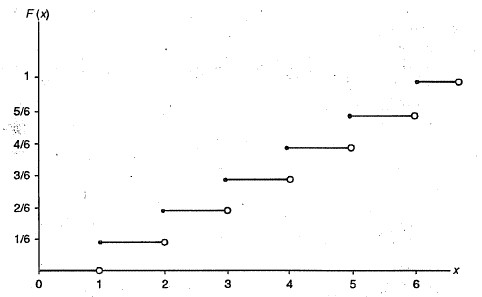
\includegraphics[height=2in]{pics/cdf.jpg}
    \caption{Graph of the CDF for rolling a single die}
    \label{cdf}
\end{figure}

\begin{theorem}
    \begin{equation*}
        P(a < X \leq b) = F (b) - F (a)
    \end{equation*}
\end{theorem}

\textbf{Proof}: Let \(I_1\) be \( (-\infty,a]\) and \(I_2\) be \(a,b]\). Then \(I_1 \text{and} I_2\) are disjoint and hence \(P(I_1)+P(I_2)=P(I_1 \cup I_2)\). But \(P(I_1 \cup I_2) = F(b) \text{and} P(I_1)=F(a)\). Hence \(P(a < X \leq B) = P(I_2) = F(b) - F(a)\).

This theorem enables us to assign probabilities to any open interval \((a,b]\)

\begin{theorem}
    For each \(x \in \mathbb{R}\), \(F(x)\) is continuous to the right of \(x\).
\end{theorem}

\textbf{Proof:} Consider \(B_n=(x,x+ \frac{1}{n}]\) for \(n>0\), which is open at the left and closed at the right. We have \(P(B_n)=F(x+ \frac{1}{n}) - F(x)\). Also, \(B_{n+1} \subset B_n\), and hence \(B_n\) is monotonic decreasing. Hence \(\lim\limits_{n \rightarrow \infty} B_n = \emptyset\); the limit set of \(B_n\) is the empty set. Therefore \(P(\lim B_n) = 0\). By Theorem 9, \(P(\lim B_n)= \lim(P(B_n))\). Hence,
\begin{equation*}
    0 = P \left(\lim\limits_{n \rightarrow \infty} B_n\right) = \lim\limits_{n \rightarrow \infty} \left[F(x + \frac{1}{n})-F(x)\right] = F(x+)-F(x)
\end{equation*}
where \(F(x+)\) is the right hand limit of \(F(x)\) at \(x\). This establishes the theorem that \(F(x)\) is right continuous of \(x\)

\begin{theorem}
    If \(F(x)\) is continuous at \(x \in \mathbb{R}\), then \(P(X=x)=0\)
\end{theorem}

\textbf{Proof:} First define \(B_n = (x-\frac{1}{n}, x+\frac{1}{n}]\). Hence, by monotonicity, as \(n \rightarrow \infty\), \(P(\lim B_n)=\lim P(B_n)\). But
\begin{equation*}
    \lim P(B_n) = \lim\limits_{n \rightarrow \infty} \left[F \left(x+\frac{1}{n}\right) - F \left(x-\frac{1}{n}\right) \right] = 0
\end{equation*}
because \(F(x)\) is continuous at \(x\). By monotonicity, \(\lim B_n = x\), and hence \(P (\lim B_n) = P(X=x)\). Hence the result that \(P(X=x)=0\) when \(F(x)\) is continuous at \(x\).

\subsection{Discrete Distributions}

A random variable \(X\) is said to have a \textbf{discrete distribution} if it can take only a finite number of different values \(x_1, x_2, ..., x_m\), or a countably infinite number of distinct points.

\begin{definition}
    For a discrete random variable \(X\), let \(f(x) = P_x(X=x=\). The function \(f(x)\) is called the \textbf{probability function} (or as PF).
\end{definition}

The relationship between a CDF and a PF is straightforward. Because \(F(x) = P(X \leq x)\), we have \(F(x) = \sum_{X \leq x} f(X)\).

The case of rolling a dice has a \textbf{uniform distribution on integers} for which \(X\) takes only the values 1,2,..., \(n\), each with equal probability \(p = \frac{1}{n}\). \(f(x)=\frac{1}{n} \text{ for } x=1,2,...,n\) and 0 elsewhere.

Every probability function involves one or more parameters that will be denoted by $\theta$. The \textbf{parameter space}, that is, the set of values $\theta$ can take, is denoted by $\Theta$. We write the probability function \(f(x; \theta), \theta \in \Theta\) and note that what we have is a \textit{a family of distributions}.

\subsubsection{The Bernoulli Distribution}

Consider an experiment which has only two outcomes, one named a \textit{success} and the other named \textit{failure}. The sample space is \(S={succes, failure}\). Let \(P(success)=p\) (and \(P(failure)=1-p\). Define a random variable \(X\) for which \(X(success)=1\) and \(X(failure)=0\). We then have \(P(X=1)=p, P(X=0)=1-p\). This can be represented in the form \(f(x;p)=p^x(1-p)^1-x\) for \(x=0,1\) and \(0 \leq p \leq 1\). This is the \textbf{Bernoulli distribution}.

\subsubsection{The Binomial Distribution}

Tossing a coin: a special case of the \textbf{binomial distribution} which arises out of a number of Bernoulli trials. Let \(p\) be the probability of success in a given trial and \(q=1-p\) the probability of failure. Assume also that (1) the probability of a success is the same in each trial and (2) the trials are independent.

The probability of a success in one trial follows the Bernoulli distribution. Hence the Binomial one has the following formula:
\begin{equation*}
\begin{split}
    f(x, \theta) &= B(x; n, p) = \binom{n}{x} p^x q^{n-x}, \\
    \text{where} \quad \binom{n}{x} &= \frac{n!}{x!(n-x)!}, \\
    x &= 0, 1, \ldots, n, \quad 0 \leq p \leq 1, \quad q = 1-p
\end{split}
\end{equation*}

It can be shown that \( \sum_{x=0}^{x=n} \binom{n}{x} p^x q^{n-x}\) is the expansion of \((p+q)^n\). Thus the binomial density is a typical term in the binomial expansion of \((p+q)^n\).

\subsection{Continuous Distributions}

A continuous random variable can take any value in a real interval.

\begin{definition}
    For a random variable \(X\) if there exists a nonnegative function \(f(x)\), defined on the real line, such that for any interval \(B\),
    \begin{equation*}
        P(X \in B)= \int_{B} f(x) dx
    \end{equation*}
    then \(X\) is said to have a \textbf{continuous distribution} and the function \(f(x)\) is called the \textbf{probability density function} or simply \textbf{density function} or PDF.
\end{definition}

\subsubsection{Uniform Distribution on an Interval}

A random variable \(X\) for which the density function \(f(x;a,b)\) is a positive constant \(c\) in the interval \(a \leq X \leq b\) is called the \textbf{uniform distribution on an interval}. For \(f(x;a,b)\) to be a PDF,
\begin{equation*}
    \int_{a}^{b} f(x; a,b) dx = 1 = \int_{a}^{b} c dx = c(b-a)
\end{equation*}
Hence \(f(x; a,b)=\frac{1}{b-a}\) uniformly in \(a \leq x \leq b\). Its distribution function is a straight line and is given by
\begin{equation*}
\begin{split}
    F(x; a,b)= \int_{a}^{x} f(x; a,b) dx = \frac{x-a}{b-a}\\
    \text{ for } a \leq x \leq b
\end{split}
\end{equation*}

\begin{figure} [H]
    \centering
    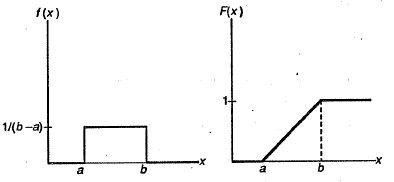
\includegraphics{pics/cdf Pdf.jpg}
    \caption{PDF and CDF of the continuous uniform distribution}
    \label{cdfpdf}
\end{figure}

\subsubsection{Normal Distribution}

The \textbf{normal (or Gaussian) distribution} has the following density:

\begin{equation*}
    f(x, \mu, \sigma) = \frac{1}{\sigma\sqrt{2 \pi}} \exp{\left[-\frac{(x-\mu)^2}{2\sigma^2}\right]} \
\end{equation*}

It's written as \(X \sim N(\mu, \sigma^2)\). The values of $\mu$ and $\sigma^2$ are generally unknown. The special case of the normal distribution for $\mu=0$ and $\sigma=0$ is known as the \textbf{standard normal} and its density function in independent of the parameters:

\begin{equation*}
    f(x)=\frac{1}{\sqrt{2\pi} e^{-x^2/2}}, -\infty < x - \infty
\end{equation*}

The CDF of the standard normal distribution is

\begin{equation*}
    F(x) = \int_{-\infty}^{x} \frac{1}{\sqrt{2\pi}} e^{-(y-\mu)^2/2 } dy
\end{equation*}

This integral doesn't have a closed form solution but requires numerical integration.

\begin{figure} [H]
    \centering
    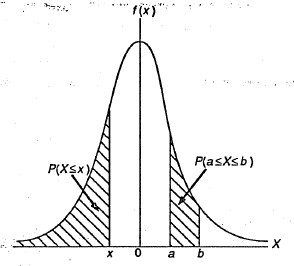
\includegraphics[height=2in]{pics/normal.jpg}
    \caption{The standard normal distribution}
    \label{normal}
\end{figure}

\subsection{Transformations of Random Variables}

Just as a requirement of a random variable was that it be event preserving, the transformation functions should also have the same property. In other words, transformations should be \textbf{measurable functions}.

\begin{definition}
    A function \(g(X)\) on \(S\) to \(\mathbb{R}\) is called \textbf{measurable function} (or $\mathcal{F}$-\textbf{measurable}) if the set \(\{x:g(x) \leq y\} \in \mathcal{F}\) for every real number \(y \in \mathcal{R}\).
\end{definition}

Thus, a function \(g(X)\) being measurable implies that we can express the probability of the event \(\{g(X) \leq y\}\) in terms of the probability of an event in $\mathcal{F}$ corresponding to \(X\).

\begin{theorem}
    Let \(F_X(x)\) be the CDF of the random variable \(X\) and let \(Y=g(X)\) be measurable, differentiable and monotonic. Then the CDF of \(Y\) is given by
    \begin{equation*}
    \begin{split}
        F_Y(y)=F_X[h(y)] \text{ if } g(X) \text{ is monotonic increasing} \\
         F_Y(y)=1-F_X[h(y)] \text{ if } g(X) \text{ is monotonic decreasing}
    \end{split}
    \end{equation*}
    where \(h(Y)\) is the inverse of \(g(X)\)
\end{theorem}

\textbf{Proof:} \(F_Y(y)= P(Y \leq y) = P[g(X) \leq y]\). Because the transformation is monotonic increasing, the event \(g(X) \leq y\) is identical to the event \(X \leq h(y)\). Hence 
\begin{equation*}
    P[g(X) \leq y] = P[X \leq h(y)] = F_X[h(y)]
\end{equation*}

\begin{theorem}
    If the assumptions of Theorem 2.4 hold, and, in addition, \(f_X(x)\) is the PDF of \(X\) and \(dx/dy \neq 0\). Then the PDF of \(Y=g(X)\) is given by
    \begin{equation*}
        \begin{split}
            f_Y(y)=f_X[h(y)] \text{ when \(X\) is discrete} \\
            f_Y(y)=f_X[h(y)] \left|dx/dy\right| \text{ when \(X\) is continuous}
        \end{split}
    \end{equation*}
\end{theorem}

\textbf{Proof:} The proof is trivial for the discrete case. \(P(Y=y) = P[X=h(y)] = f_X[h(y)]\). For a continuous random variable the PDF is the derivative of the CDF and hence,
\begin{equation*}
    f_Y(y)= \frac{d}{dy} F_Y(y)
\end{equation*}
But \(F_Y(y) = F_X[h(y)]\) by Theorem 2.4. That is
\begin{equation*}
    F_Y(y)= \int_{- \infty}^{h(y)} f_X(x) dx
\end{equation*}
Differentiating with respect to \(y\) and using the chain rule,
\begin{equation*}
    f_Y(y)=f_X[h(y)] h'(y)
\end{equation*}
But \(h'(y)=dx/dy\). Because \(f_Y(y)\) must be nonnegative, we have to use the absolute value of the derivative. Hence
\begin{equation*}
    f_Y(y)=f_X[h(y) \left|dx/dy\right|
\end{equation*}


\subsection{Characteristics of functions}

The probability density and the cumulative distribution functions determine the probabilities of random variables at various points or in different intervals. Now we're focusing on numerical measures that characterize a distribution.

\subsubsection{The Stieltjes Integral}

First we go through the definition of the Riemann integral (the traditional one). Consider the closed interval \([a,b]\) for any pair of real numbers such that \(a<b\), and a single valued function \(g(x)\) bounded in \([a,b]\). We can subdivide the interval into a number of them by inserting points \(x_i\) such that
\begin{equation*}
    a = x_0 < x_1 < x_2 < \dots < x_n = b
\end{equation*}
The subdivision is referred to as a \textbf{partition} and the largest of the lengths of the intervals (\(\Delta x_i = x_i - x_{i-1})\) as the \textbf{norm} of the partition, noted as \(||\Delta x||\). Lew \(\omega_i\) be any point in \([x_{i-1},x_i]\). Next construct the following sum (Riemann sum):
\begin{equation*}
    \sum g(\omega_i) \Delta x_i = \sum g(\omega_i) (x_i - x_{i-1})
\end{equation*}
If the limit of the sums as the norm of the partition goes to zero exists, it is called the Riemann integral of \(g(x)\). It is written as
\begin{equation*}
    \int_{b}^{a} (x)dx= \lim\limits_{||\Delta x|| \rightarrow o} \sum g (\omega_i) \Delta_i
\end{equation*}
We could replace \(\Delta x_i\) by \(\Delta F(x) = F (x_i) - F(x_{i-1}\), where \(F(x)\) is any single valued function. Thus, if the limit exists, the analogous integral is
\begin{equation*}
    \int_{b}^{a} g(x)dF= \lim\limits_{||\Delta F(x)|| \rightarrow o} \sum g (\omega_i) [F(x_i)-F(x_{i-1})]
\end{equation*}
The above is called the \textbf{Stieltjes integral}. We would choose \(F(x)\) to be the cumulative distribution function. The advantage of the Stieltjes integral with the CDF is that we don't have to distinguish between a continuous and a discrete random variable.

\subsubsection{Mathematical Expectation}

\begin{definition}
    Let \(X\) be a random variable on \(S, \mathcal{F}, P\) with \(f(x)\) as the PF or PDF, and \(g(x)\) be a single valued function. If the Stieltjes integral \(\int_{-\infty}^{+\infty} g(x) dF\) exists, it is called the \textbf{expected value} of \(g(X)\) and is denoted by \(E[g(X)]\). In the case of a discrete random variable this takes the form \(E[g(X)] = \sum_i g(x_i)f(x_i)\) and in the continuous case, \(E[g(X)]= \int_{-\infty}^{+\infty} g(x) f(x) dx \)
\end{definition}
It's basically a weighted average of \(g(X)\), the weights being the corresponding probabilities.

\subsubsection{Mean of a Distribution}

The expected value of \(X\) is a measure of central location and is called the \textbf{mean of a distribution}. \(\mu = E(X)\).

\begin{theorem}
\begin{enumerate} 
    \item If \(c\) is a constant, \(E(c)=c\)
    \item If \(c\) is a constant, \(E[c g(x)]=c E[g(x)]\)
    \item \(E[u(X)+v(X)] = E[u(X)]+E[v(X)]\)
    \item \(E(X-\mu)=0\), where \(\mu=E(X)\)
\end{enumerate}
\end{theorem}

\subsubsection{Moments of a Distribution}

A generalization of the mean is to raise \(X\) to any positive integer power greater than 1, that is, set \(m=2,3, \dots,\) and compute
\begin{equation*}
    E(X^m)=\int_{-\infty}^{\infty} x^m dF
\end{equation*}

If the integral exists, it's called the \textbf{nth moment around the origin} and is denoted by \(\mu_m')\). Around the mean we can obtain the \textbf{central moments} or moments around the mean, which are \(\mu_m\). Thus,
\begin{equation*}
    E(X^m)=\int_{-\infty}^{\infty} (x-\mu)^m dF
\end{equation*}

The mean and higher moments may not always exist (Cauchy distribution).

\subsubsection{Variance and Standard Deviation}

\(E[(X-\mu)^2\) is the second moment of a distribution, where \(E(x)=\mu\) and it's called the \textbf{variance of a distribution}. The positive square root is called the \textbf{standard deviation}.
\begin{equation*}
    \sigma^2= E[(X-\mu)^2] = Var(X) = \int(x-\mu)^2 dF
\end{equation*}

\(X-\mu\) us the deviation of \(X\) from its mean. \(E[(X-\mu)^2]\) is an average of the squared deviation from the mean. Thus \(\sigma^2\) is a measure of the dispersion of a distribution that can be written in another form also:
\begin{equation*}
    \begin{split}
        \sigma^2 = E[(X-\mu)^2] = E(X^2-2X\mu+\mu^2) \\
        = E(X^2)-2\mu E(X)+E(\mu^2) = E(X^2)-\mu^2 = \mu_2 - \mu^2
    \end{split}
\end{equation*}

\begin{theorem}
    If \(E(X)=\mu\) and \(Var(X)=\sigma^2\), and \(a\) and \(b\) are constants, then \(Var(a+bX)=b^2\sigma^2\)
\end{theorem}

\textbf{Proof:} Let \(Y=a+bX\). Then \(E(Y)=a+b E(X) = a + b\mu\). Hence \(Y-E(Y)=b(X-\mu)\).
\begin{equation*}
    Var(Y)=E[Y-E(Y)]^2=E[b^2(X-\mu)^2]=b^2\sigma^2
\end{equation*}

\subsubsection{Chebyshev's Inequality}
\begin{theorem}
    Let \(b\) be a positive constant and \(h(X)\) be a nonnegative measurable function of the random variable \(X\). Then
    \begin{equation*}
        P[h(X) \geq b] \leq \frac{1}{b} E[h(X)]
    \end{equation*}
    \textbf{Corollary: Chebyshev's inequality}. For any constant \(c>0\) and \(\sigma^2=Var(X)\),
    \begin{enumerate}
        \item \(P[|X-\mu| \geq c] \leq \sigma^2/c^2\)
        \item \(P[|X-\mu| \leq c] \geq 1-\frac{\sigma^2}{c^2}\)
        \item \(P[|X-\mu| \geq k\sigma] \leq 1/k^2\)
    \end{enumerate}
\end{theorem}

\textbf{Proof:} \begin{equation*}
    E [h(X)] = \int h(X) dF = \int_{h(x) \geq b} h(x) dF + \int_{h(x)<b} h(x) dF \geq \int_{h(x) \geq b} h(x) dF
\end{equation*}
because \(h(X)\) is a nonnegative function. When \(h(X) \geq b\),
\begin{equation*}
    E[h(X)] \geq \int_{h(x) \geq b} b  dF = b P[h(X) \geq b] 
\end{equation*}

Therefore, \(P[h(X) \geq b] \leq \frac{1}{b} E[h(X)]\).

\textbf{Corollary:} Let \(h(X) = (X-\mu)^2\) and \(b=c^2\). Then
\begin{equation*}
    P[(X-\mu)^2 \geq c^2] = P[|X-\mu| \geq c]
\end{equation*}
Hence
\begin{equation*}
\begin{split}
    P[(X-\mu)^2 \geq c^2] \leq \frac{1}{c^2} E[(X-\mu)^2] \\
    E[(X-\mu)^2] = \sigma^2 \\
    P[(X-\mu)^2 \geq c^2] \leq \frac{1}{c^2} \sigma^2 \\
    P[(X-\mu)^2 \geq c^2] \leq \frac{\sigma^2}{c^2} \\
    P[(X-\mu)^2 \geq c^2] = P[|(X-\mu)|\geq c] \\
    P[|(X-\mu)|\geq c] \leq \frac{\sigma^2}{c^2}
\end{split}
\end{equation*}

If \(c=k\sigma\), the third alternative form follows:
\begin{equation*}
\begin{split}
        P[|(X-\mu)|\geq k\sigma] \leq \frac{\sigma^2} {k^2\sigma^2} \\
         P[|(X-\mu)|\geq k\sigma] \leq \frac{1} {k^2}
\end{split}
\end{equation*}

Chebyshev's inequality states that for any distribution the probability of \(X\) falls outside a 2$\sigma$ interval form the mean is $\leq 1/4$, outside a 3$\sigma$ range is $\leq 1/9$. Thus $\sigma$ controls the dispersion of \(X\).

\subsubsection{Approximate Mean and Variance of \(g(X)\)}

There might be cases in which the mean and variance of a measurable function \(g(X)\) of a random variable \(X\) may not be readily obtainable; e.g. for \(g(X) = \sqrt{X}\), the integral corresponding to \(E[g(X)]\) doesn't have a tractable expression.

Suppose \(X\) is a random variable defined on \((S, \mathcal{F},P)\) with \(E(X)=\mu\) and \(Var(X)=\sigma^2\), and let \(g(X)\) be a differentiable and measurable function of \(X\). We take a linear approximation of \(g(X)\) in the neighborhood of $\mu$:
\begin{equation*}
    g(X) \approx g(\mu)+g'(\mu)(X-\mu)
\end{equation*}
provided \(g(\mu)\) and \(g'(\mu)\) exist. The second term has zero expectation, hence \(E[g(X)] \approx g(\mu)\). By Theorem 16, (\(Var(a+ bX) = b^2\sigma^2\)), we have
\begin{equation*}
\begin{split}
    Var[g(x)] = Var[g(\mu)] + Var[g'(\mu)(X-\mu)] \\
    Var[g(X)] = \sigma^2[g'(\mu)]^2
\end{split}
\end{equation*}

In the case of \(g(X)=\sqrt{X}\), the approximate mean is \(\sqrt{\mu}\) and the approximate variance is \(\sigma^2/(4\mu)\). 

What we use is a linear approximation which may be grossly inaccurate if the curvature of the function \(g(X)\) is high.

\subsubsection{Mode of a Distribution}

The point(s) for which \(f(x)\) is maximum is(are) called the \textbf{mode}. It's the most frequently observed value of \(X\).

\subsubsection{Median, Upper and Lower Quartiles and Percentiles}

A value of \(x\) such that \(P(X<x) \leq 1/2\) and \(P(X \leq x) \geq 1/2\) is called the \textbf{median} of the distribution. It's the point on either side of which lies 50 percent of the distribution. It's often preferred over the mean as an average measure because the arithmetic average can be misleading if extreme values are present.

Instead of 1/2, we could use any probability between 0 and 1. The point(s) with an area of 1/4 to the left is (are) called the \textbf{lower quartile(s)}, and the point(s) corresponding to 3/4 is (are) the \textbf{top quartile(s)}.For any probability \(p\), the values of \(x\) for which the area to the right is \(p\) are called the \textbf{upper \(p\)th percentiles} (also referred to as quantiles).

\subsubsection{Coefficient of Variation}

It's defined as \(\sigma/\mu\). It is a measure of the dispersion of a distribution \textit{relative to its mean} and is useful in the estimation of relationships. 

\subsubsection{Skewness and Kurtwosis}

If a continuous density \(f(x)\) has the property that \(f(\mu+a)=f(\mu-a)\) for all \(a\), then \(f(x)\) is said to be \textbf{symmetric around the mean}. If a distribution is not symmetric around the mean, then it's called \textbf{skewed}. We have two types of skewness, positive (long tail  to the right) and negative (long tail to the left). A commonly used measure of skewness is \(E[(X-\mu)^3/\sigma^3]\).

\begin{figure} [H]
    \centering
    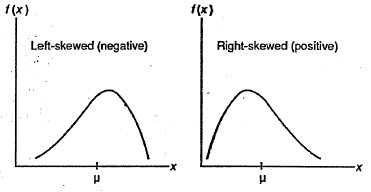
\includegraphics{pics/skewness.jpg}
    \caption{Skewness of a distribution}
    \label{skew}
\end{figure}

The peakedness of a distribution is called \textbf{kurtosis}. A narrow distribution is called \textbf{leptokurtic} and a flat distribution is called \textbf{platykurtic}. One measure of kurtosis is \(E[(X-\mu)^4/\sigma^4]\). The value \(E[(X-\mu)^3/\sigma^3]-3\) is often referred to as \textbf{excess kurtosis}.

\begin{figure} [H]
    \centering
    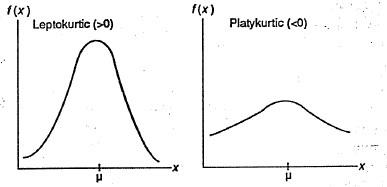
\includegraphics{pics/kurtwosis.jpg}
    \caption{Kurtosis of a distribution}
    \label{kurt}
\end{figure}

\subsection{Generating Functions}

\subsubsection{The Moment Generating Function}

\begin{definition}
    The function \(m(t)=E(e^{Xt})=\int_{- \infty}^{+ \infty} e^xt dF\) is called the \textbf{moment generating function} (also known as Laplace transform) of \(X\). The function is defined for those values of \(t\) for which the integral exists.
\end{definition}

\subsubsection{The Characteristic Function}

\begin{definition}
    The function \(\phi(t)=E(e^{iXt})\) where \(i^2=-1\), that is, the complex \(i\), is called the \textbf{characteristic function (CF)} of \(X\).
\end{definition}

Using power series expansions of \(e^{ixt},\sin{xt} \text{ and } \cos{xt}\), it is verified that \(e^{ixt}=\sin{xt} + \cos{xt}\). Therefore

\begin{equation*}
    \phi(t)= \int_{- \infty}^{+ \infty} \cos{(xt)} dF + i  \int_{- \infty}^{+ \infty} \sin{(xt)} dF
\end{equation*}

Each of the integrals is called a \textbf{Fourier transform} of \(f(x)\). The characteristic function always exists even though the moment generation function may not. The power series expansion of \(e^{iXt}\) is

\begin{equation*}
    e^{iXt}=\sum_{r=0}^{\infty} \frac{(iXt)^r}{r!}
\end{equation*}

Therefore, the characteristic function can also be written as

\begin{equation*}
    \phi(t)=\sum_{r=0}^{\infty} \frac{E[(iXt)^r]}{r!} = \sum_{r=0}^{\infty} \frac{i^r t^r}{r!} \mu_r'
\end{equation*}
where \(\mu_r'=E(X^r)\) is the rth moment of \(X\).

\begin{theorem}
    A characteristic is uniformly continuous on the real line
\end{theorem}

\textbf{Proof:} 
\begin{equation*}
    \phi(t+h)-\phi(t)=\int e^{ixt} (e^{ixh}-1) f(x) dx
\end{equation*}
Because \(|e^{ixt} \leq 1\), \(|\phi(t+h)-\phi(t)| \leq \int |e^{ixh}-1| f(x) dx\). For a given \(\varepsilon\), choose \(A\) large such that \(\int_{|x|>A}f(x)dx < \varepsilon/4\) and a \(h\) small so that for \(|x| \leq A, |e^{ixh}-1| < \varepsilon/4A\). We have
\begin{equation*}
    |\phi(t+h)-\phi(t)| \leq \int_{-A}^{+A} |e^{ixh}-1|f(x)dx + \int_{|x|>A} |e^{ixh}-1| f(x) dx
\end{equation*}
The first integral is \(< \varepsilon/2\) because \(f(x) \leq 1\), and when \(|x| \leq A, |e^{ixh}-1| < \varepsilon/4A\). When \(|x|>A, |e^{ixh}-1| \leq 2\), which is attained when \(xh=\pi\). Therefore the second integral is less than \(\varepsilon/2\), making the total less than \(\varepsilon\). Hence \(\phi(t)\) is uniformly continuous.

Assuming that \(\phi(t)\) is differentiable under the integral sign we get
\begin{equation*}
    \phi'(t)=\int_{-\infty}^{\infty} e^{ixt} ix dF
\end{equation*}
It follows that \(\phi'(0)=i E(X)\).
\begin{equation*}
    \phi^r(0)= \underset{0}{\left[\frac{d^r\phi(t)}{dt} \right]} = i^r\mu_r'
\end{equation*}
provided that the rth derivative exists. Thus moments exist if and only if the corresponding derivatives of \(\phi(t)\) exist at \(t=0\).

\begin{theorem} \textbf{Uniqueness theorem}.
    Two distribution functions are identical if and only if their characteristic functions are also identical
\end{theorem}
Implies that corresponding to each characteristic function \(\phi(t)\) there exists a unique distribution function \(F(x)\) having their characteristic function.

\begin{theorem} \textbf{Inversion theorem}. Let \(F(x)\) be the distribution function (continuous), and \(\phi(t)\) be the corresponding characteristic function. Then for any \(x,h \in \mathbb{R}\),
\begin{equation*}
    F(x+h)-F(x-h)= \lim_{T \rightarrow \infty} \frac{1}{2\pi} \int_{-T}^{T} \left[\frac{1-e^{-ith}}{it}\right] e^{-itx} \phi(t) \, dt
\end{equation*}
provided that \(x-h\) and \(x+h (h>0)\) are continuity points of \(F(x)\).
\end{theorem}

\begin{theorem} \textbf{Inversion formula}.
    If a characteristic function \(\phi(t)\) is absolutely integrable over \((-\infty,+\infty)\), then the corresponding distribution function \(F(x)\) is absolutely continuous and the corresponding density function is
\begin{equation*}
    f(x)=F'(x)=\frac{1}{2\pi} \int_{-\infty}^{\infty} e^{-itx} \phi(t) dt
\end{equation*}
\end{theorem}

From the above theorems that corresponding to each characteristic function \(\phi(t)\) there exists a unique distribution function \(F(x)\) having that characteristic function and that it is often possible to obtain the corresponding density function \(f(x)\) also.

\section{Some Special Distributions}

\subsection{Discrete Distributions}

\subsubsection{The Binomial Distribution}

This distribution arises when there are only two possible outcomes to an experiment, one labeled a \textit{success} and the other labeled a \textit{failure}. If \(p\) is the probability of a success, we have the following:

\begin{equation*}
\begin{split}
    f(x:\theta)=B(x;n,p) = \binom{n}{x} p^x q^{n-x} = \frac{n!}{x!(n-x)!} p^x q^{n-x}\\
    x = 0,1,...,n ; 0 \leq p \leq 1; q = 1-p \\
    \phi(t) = (q+pe^{it})^n ; E(X) = np; Var(X)=npq
\end{split}
\end{equation*}

\subsubsection{Simple Random Walk}

The probability of an upward movement is \(p\) and that for a downward movement is \(1-p\). Let \(X\) be the change in the price of the stock after \(n\) trading days; what is \(f(x)\)?

After \(n\) days, \(x\) can range from \(-n\) to \(n\). If there are \(k\) upward movements and \(n-k\) downward movements, then the probability of the outcome is \( \binom{n}{k} p^k(1-p)^{n-k}\) and \(x = k-(n-k)= 2k-n\) which implies \(k=(x+n)/2\). Hence,
\begin{equation*}
\begin{split}
    f(x)=P(k \text{ successes}) = \left[\binom{n}{(x+n)/2} p^{(x+n)/2} (1-p)^{n-(x+n)/2} \right] \\
    x=-n,\dots,-2,-1,0,1,2,\dots,n
\end{split}
\end{equation*}

\subsubsection{Negative Binomial Distribution}

In a binomial experiment, let \(Y\) be the number of trials to get exactly \(k\) successes, there must be \(k-1\) successes in \(y-1\) trials and the next outcome must be a success. Therefore,
\begin{equation*}
    f(y;k,p) = \binom{y-1}{k-1} p^k q^{y-k} ; y=k,k+1,k+2,\dots
\end{equation*}
Let \(X=Y-k\) be the number of failures until \(k\) successes have been obtained. The density function of \(X\) is known as the \textbf{negative binomial}.
\begin{equation*}
    f(x;k,p)=\binom{x+k-1}{n-1} p^k q^x ; x=0,1,2,\dots
\end{equation*}

\subsubsection{Geometric Distribution}

Let \(X\) be the number of the trial at which the first success occurs. The distribution of \(X\) is a \textbf{geometric distribution}. Density function:

\begin{equation*}
    f(x;p)=p (1-p)^{x-1} ; x=1,2,3,\dots
\end{equation*}

\subsubsection{Poisson Distribution}

Consider the binomial distribution \(B(x;n,p)\) and let \(n \rightarrow \infty, p \rightarrow 0\) such that \(np=\lambda(>0) \text{ for all } n \text{ and } p\). Thus the probability of a success is very small and the number of trials is large. What's the distribution?

\begin{equation*}
    \begin{split}
        B(n,p) = \frac{n(n-1)\dots(n-x+1)}{x!} p^x (1-p)^{n-x} \\
        = \frac{n(n-1)\dots(n-x+1)}{x!} \frac{\lambda^x}{n^x} \left(1-\frac{1}{\lambda} \right)^{n-x} \\
        = \frac{1 \left(1-\frac{1}{n}\right) \left(1-\frac{2}{n}\right) \dots \left(1-\frac{x-1}{n}\right)}{x!} \lambda^x \left[\left(1-\frac{\lambda}{n} \right)^n\right]^{\frac{n-x}{n}}
        \end{split}
\end{equation*}

Now let \(n \rightarrow \infty\). We get \(\lim\limits_{n \rightarrow \infty} B(n,p) = (\lambda^x e^{-\lambda})/x!\) because \(\lim\limits_{n \rightarrow \infty} [1-(\lambda/n)]^n=e^{-\lambda}\). Thus we get

\begin{equation*}
    f(x;\lambda) = \frac{e^{-\lambda} \lambda^x}{x!}; x=0,1,2,\dots
\end{equation*}
which is known as the \textbf{Poisson Distribution}. We can verify that \(\sum_{0}^{\infty} f(x,\lambda)=1\).
\begin{equation*}
    \sum_{0}^{\infty} e^{-\lambda} \frac{\lambda^x}{x!} = e^{-\lambda} \left[1+\frac{\lambda}{1!}+\frac{\lambda^2}{2!} +\dots\right] = e^{-\lambda}e^\lambda=1
\end{equation*}
Thus \(f(x;\lambda)\) is indeed a PF.

\subsubsection{Hypergeometric Distribution}

Let there be \(a\) objects in a certain class and \(b\) in another class. We draw a random sample of size \(n\) without replacement. What is the probability of observing \(x\) from class A? First there are \(\binom{a+b}{n}\) ways of drawing \(n\) objects from \(a+b\) objects, which is the total number of possible outcomes. To get \(x\) from class A, there are \(\binom{a}{x}\) possible ways. For \textit{each} such outcome, there are \(\binom{b}{n-x}\) possible ways of drawing from B. Thus there are \(\binom{a}{x}\ \binom{b}{n-x}\) ways of drawing \(x\) from \(A\) and \(n-x\) from \(B\). Therefore the required probability is
\begin{equation*}
    f(x;n,a,b)=\frac{\binom{a}{x} \binom{b}{n-x}}{\binom{a+b}{n}}
\end{equation*}
where \(x=0,1,2,\dots,n; 0 < a, b\leq n; a \text{ and } b \text{ are integers.}\) This distribution is the \textbf{hypergeometric distribution}

\subsection{Continuous Distributions}

\subsubsection{Uniform Distribution on an Interval}

Arises when the probability density function is a constant over an interval.
\begin{equation*}
\begin{split}
    f(x)=\frac{1}{b-a}; a \leq x \leq b \\
    E(X)=\frac{a+b}{2}; Var(X)=\frac{(b-a)^2}{12}
\end{split}
\end{equation*}

\subsubsection{Normal Distribution}

The normal distribution \(N \sim (\mu, \sigma^2)\) is symmetric around its mean and is distributed with a bell shape. 
\begin{equation*}
    \begin{split}
        f(x, \mu, \sigma) = \frac{1}{\sigma\sqrt{2 \pi}} \exp\left[-\frac{(x-\mu)^2}{2\sigma^2}\right]; -\infty < x < \infty \\
        E(X) = \mu; Var(X)=\sigma^2 \\
        \phi(t)=\exp[i\mu t-\frac{\sigma^2t^2}{2}]
    \end{split}
\end{equation*}


\subsubsection{Exponential Distribution}

The distribution \(f(x;\theta)=(1/\theta)e^{-x/\theta}\) for \(x>0\) and \(\theta>0\), is called the \textbf{exponential distribution}. Its CDF is \(F(x,\theta)=1-e^{-x/\theta}\).

It can be shown that it provides an appropriate model for the lifetime of an equipment. Suppose that the probability that a given equipment will fail during a small time interval \(\Delta x\) is \((1/\theta)\Delta x\), independent of \(x\). Now divide 0 to \(x\) into \(n\) intervals with \(\Delta x=x/n\). The probability that an equipment will \emph{not} fail in \emph{one} of these intervals is \(1-x/n\theta\). Hence it will not fail in 0 to \(x\) with a probability \([1-(x/n\theta)]^n\). As \(n \rightarrow \infty\), we get \(\lim\limits_{n \rightarrow \infty} [1-(x/n\theta)]^n=e^{-x/\theta}\). Thus \(F(x;\theta)\) is the probability that a given equipment will fail in the interval 0 to \(x\).

\subsubsection{Weibull Distribution}

An alternative used in the cases in which the conditions for the exponential distribution are not met is the \textbf{Weibull distribution}, which has the density function
\begin{equation*}
    f(x;a,b) = abx^{b-1}e^{-ax^b}; \hspace{0.5cm} x>0 \hspace{0.5cm}; a,b>0
\end{equation*}

\subsubsection{LogNormal Distribution}

A random variable X has a \textbf{standard lognormal distribution} if \(Z=\ln X\) has the standard normal distribution.
\begin{equation*}
    f_Z(z)=\frac{1}{\sqrt{2\pi}}e^{-z^2/z} \hspace{0.5cm} -\infty < z < \infty
\end{equation*}
By Theorem 13, 
\begin{equation*}
    f_X(x)=\frac{1}{\sqrt{2\pi}}\left[e^{-(\ln x)^2/2} \right] \frac{1}{x} \hspace{0.5 cm} 0 < x < \infty
\end{equation*}

It is useful to derive the \(m\)th moment of a lognormal random variable, that is, \(\mu_m'=E(X^m)\). We have
\begin{equation*}
    E(X^m)=\int_{0}^{\infty} x^m \frac{1}{\sqrt{2\pi}}e^{-z^2/2} \frac{1}{x} dx
\end{equation*}
Making the substitution \(x=\ln x\) we get
\begin{equation*}
\begin{split}
      E(X^m)=\int_{-\infty}^{\infty} e^{mz} \frac{1}{\sqrt{2\pi}}e^{-z^2/2} dz \\
      = \int_{-\infty}^{\infty} \frac{1}{\sqrt{2\pi}}e^{-[(z-m)^2-m^2]/2} dz = e^{m^2/2}
\end{split}
\end{equation*}
because the rest of the integral is 1. It follows from this that
\begin{equation*}
    E(X)=\sqrt{e} \hspace{0.5cm} Var(X)=e^2-e
\end{equation*}

\subsubsection{Pareto Distribution}

The lognormal distribution is often used to model the distribution of incomes, but it's been found to approximate incomes in the middle range very well and fail in the upper tail. A more appropriate distribution is the \textbf{Pareto Distribution} which has the density
\begin{equation*}
    f(x;\alpha)=\frac{\alpha}{(1+x)^{(\alpha+1)}} \hspace{0.5cm} 0 < x < \infty \hspace{0.5cm} \alpha>0
\end{equation*}

\subsubsection{Extreme Value Distribution}

For modeling extreme values we can use the \textbf{extreme value distribution} which has the following density
\begin{equation*}
    f(x)=e^{-x} \exp [-e^-x] \hspace{0.5cm} -\infty < x < \infty
\end{equation*}

\subsubsection{Logistic Distribution}

The distribution such that \(F(x)=1/(1+e^{-x})\) is called the \textbf{logistic distribution}. Its density function is
\begin{equation*}
    f(x)=F'(x)=\frac{e^{-x}}{(1+e^{-x})^2} \hspace{0.5cm} -\infty<x<\infty
\end{equation*}

Frequently used to model growth relationships: initially slow sales, a period of very rapid increase in sales, then a tapering off of the growth rates.

\subsubsection{Cauchy Distribution}

The standard \textbf{Cauchy distribution} has the density function
\begin{equation*}
    f(x)=\frac{1}{\pi(1+x^2)} \hspace{0.5cm} -\infty<x<\infty
\end{equation*}

\subsubsection{Gamma Distribution}

The density function is 
\begin{equation*}
    f(x;\alpha,\beta)=\frac{1}{\beta^\alpha \Gamma(\alpha)} x^{\alpha-1} e^{-(x/\beta)} \hspace{0.5cm} x>0, \hspace{0.25cm} \alpha,\beta>0
\end{equation*}
where \(\Gamma(\alpha)\) is known as the \textbf{gamma function} \(\int_{0}^{\infty} y^{\alpha-1}e^{-y}dy\) for \(\alpha>0\). It's a useful two parameter family of distributions. It's been found to be a better approximation to the distribution of lifetime of equipment than the exponential. When \(\alpha=1\), the Gamma variate reduces to the exponential case.

\begin{theorem}
    For the gamma function defined as \(\Gamma(\alpha)=\int_{0}^{\infty} x^{\alpha-1}e^{-x}dx\),
    \begin{itemize}
        \item \(\Gamma(1)=1\) and \(\Gamma(1/2)=\sqrt{\pi}\)
        \item \(\Gamma(\alpha+1)=\alpha\Gamma(\alpha)\) and hence, if \(\alpha\) is a positive integer, then \(\Gamma(\alpha+1)=\alpha!\)
    \end{itemize}
\end{theorem}

\textbf{Proof:} 
\begin{itemize}
    \item[a)]  \begin{equation*}
    \begin{split}
        \Gamma(1)=\int_0^{\infty} e^{-x} dx = [-e^{-x}]\bigg|_{0}^{\infty} = 1 \\
        \Gamma(1/2) = \int_0^{\infty} x^{-1/2} e^{-x} dx 
    \end{split}
    \end{equation*}
    Let \(x=y^2/2\). Then
    \begin{equation*}
        \Gamma(1/2) = \int_0^{\infty} \frac{\sqrt{2}}{y} y e^{-y^2/2} dy
    \end{equation*}
    But \(\int_{-\infty}^{\infty} \frac{1}{2\pi} e^{-y^2/2} dy=1\), because the integrand is \(N(0,1)\). Also, by symmetry, \(\int_0^{\infty} \frac{1}{2\pi} e^{-y^2/2} dy=1/2\). Using this above we get \(\Gamma(1/2)=\sqrt{\pi}\)
    \item[b)] Integrate \(\Gamma(\alpha+1)\) by parts. We get
    \begin{equation*}
    \begin{split}
        \Gamma(\alpha+1)=\int_0^{\infty} x^\alpha e^{-x} dx\\
        = [-x^\alpha e^{-x}]\bigg|_0^{\infty} + \int_0^{\infty} \alpha x^{\alpha-1}e^{-x}dx=\alpha \Gamma(\alpha)
    \end{split}
    \end{equation*}
    because the first term is zero. If \(a\) is a positive integer, this recursive formula can be repeatedly applied to give \(\Gamma(\alpha+1)=\alpha!\)
\end{itemize}

\subsubsection{Beta Distribution}

The density function has the form
\begin{equation*}
    f(x)=\frac{1}{B(m,n)} x^{m-1}(1-x)^{n-1} \hspace{0.5cm} 0<x<1, \hspace{0.25cm} m,n>0
\end{equation*}
where the constant is
\begin{equation*}
    B(m,n)=\int_0^{1} x^{m-1}(1-x)^{n-1}
\end{equation*}
which is known as the \textbf{beta function}. It's flexible and can be used to model several different shapes. If \(m=n=1\), this reduces to the uniform distribution. It can be shown to satisfy the equation
\begin{equation*}
    B(m,n)=\frac{\Gamma(m)\Gamma(n)}{\Gamma(m+n)}
\end{equation*}

\subsection{Extensions of distributions}

\subsubsection{More General Parametrization}

We list a number of extensions that make the families of densities more flexible and richer in parametrization.

\begin{itemize}
    \item \textit{Exponential}:
    \begin{equation*}
        f(x;\mu, \theta)=\frac{1}{\theta} e^{-(x-\mu)/\theta} \hspace{0.5cm} x>\mu,\theta>0
    \end{equation*}
    \item \textit{Pareto}:
    \begin{equation*}
        f(x;\theta, x_0)=\frac{\theta}{x_0}[\frac{x_0}{x}]^{\theta+1} \hspace{0.5cm} x>x_0,\theta>0
    \end{equation*}
    \item \textit{Logistic}:
    \begin{equation*}
    \begin{split}
        f(x; \alpha,\beta)=\frac{(1/\beta)e^{-(x-\alpha)/\beta}}{[1+e^{-(x-\alpha)/\beta}]^2} \\
        -\infty<x<\infty, -\infty<\alpha<\infty, \beta>0
    \end{split}
    \end{equation*}
    \item \textit{Cauchy}:
    \begin{equation*}
    \begin{split}
        f(x)=\frac{1}{\pi\beta[1+\frac{(x-\alpha)}{\beta}]^2} \\
        -\infty<x<\infty, -\infty<\alpha<\infty, \beta>0
    \end{split}
    \end{equation*}
    \item \textit{Lognormal:}
    \begin{equation*}
    \begin{split}
       f(x)=\frac{1}{\sqrt{2\pi}(x-\theta)} e^{-[\ln(x-\theta)-\mu]^2/(2\sigma^2)} \\
       x > \theta, -\infty < \mu < \infty, \sigma>0
    \end{split}
    \end{equation*}
    \item \textit{Pearson family:} \(f(x)\) satisfies the following differential equation:
    \begin{equation*}
        \frac{1}{f(x)} \frac{df}{dx} = \frac{x+a}{b_0+b_1x+b_2x^2}
    \end{equation*}
    where \(a\) and \(b\) are constants. Several of the densities we specified earlier are special cases of the Pearson family, which covers a wide variety of shapes in probability distributions and is widely used in \textbf{curve fitting}.
    \item \textit{Exponential family:} 
    \begin{equation*}
    f(x;\theta)=\exp[U(x)+\sum_{i=1}^{i=k} T_i(x)A_i(\theta)+B(\theta)]    
    \end{equation*}
    \end{itemize}

\subsubsection{The Hazard Function}

Studies on reliability, instantaneous failure rates, layoffs, and so on often use a function called the \textbf{hazard function} which is closely related to the PDF and CDF of a distribution. The hazard function is defined as
\begin{equation*}
    h(x)=\frac{f(x)}{1-F(x)} \hspace{0.5cm} x>\alpha
\end{equation*}
where \(f(x)\) and \(F(x)\) are the PDF and CDF of the random variable \(x\) and \(\alpha\) is a parameter. The hazard function is thus a conditional density function.

\section{Multivariate Distributions}

\subsection{Bivariate distribution}

\begin{definition}
    Let \(X\) and \(Y\) be two random variables. Then the function \(F_{XY}(x,y)=P(X\leq x \text{ and } Y \leq y)\) is called the \textbf{joint distribution function}.
\end{definition}

The joint distribution has the following properties:
\begin{itemize}
    \item [1.] \(F_{XY} (x,\infty)\) and \(F_{XY}(\infty,y)\) are univariate distribution functions, as functions of \(x\) and \(y\) respectively.
    \item[2.] \(F_{XY}(-\infty,y)=F_{XY}(x,-\infty)=0\) 
\end{itemize}

\begin{definition} \textbf{Joint density or probability function} \\
   \centering {Discrete probability function: \(f_{XY}(x,y)=P(X=x,Y=y)\) \\
    Continuous density function: \(f_{XY}=\frac{\partial^2 F(x,y)}{\partial x \partial y}\) \\
    and hence: \(F_{XY} (x,y) \int_{-\infty}^{x} \int_{-\infty}^{y} f_{XY}(u,v) du dv\)}
\end{definition}

For the joint density function to exist in the continuous case, \(F_{XY}(x,y)\) must have continuous cross partial derivatives. In the univariate case, if \(\Delta x\) is a small increase of \(x\), then \(f_x(x)\Delta x\) is the approximate probability that \(x-1/2 \Delta x < X < x+1/2 \Delta x\). In a bivariate distribution, \( f_{XY}(x,y)\Delta x \Delta y\) is the approximate probability that \(x-1/2 \Delta x < X < x+1/2 \Delta x\) and \(y-1/2 \Delta y < Y < y+1/2 \Delta y\). The density function satisfies the conditions \(f_{XY} (x,y= \geq 0\) and \(\int_{-\infty}^{\infty} \int_{-\infty}^{\infty} dF(x,y)=1\), where \(dF(x,y)\) is the bivariate analog of \(dF(x)\).


\begin{definition} \textbf{Marginal density} \\
    If \(X\) and \(Y\) are discrete random variables, then \(f_X(x)=\sum_y f_{XY}(x,y)\) is the \textbf{marginal density of X} and \(f_Y(y)=\sum_x f_{XY}(x,y)\) is the \textbf{marginal density of Y}. In the continuous case, \(f_X(x)=\int f_{XY}(x,y)dy\) is the marginal density of \(X\) and \(f_Y(y)=\int f_{XY}(x,y)dx\) is the marginal density of \(Y\).
\end{definition}

\begin{definition} \textbf{Conditional density} \\
    The \textbf{conditional density of \(Y\) given \(X=x\)} is defined as \(f_{Y|X} (x,y)=f_{XY}(x,y)/f_X(x)\) provided \(f_X(x) \neq 0\). The conditional density of \(X\) given \(Y=y=\) is \(f_{X|y} (x,y)=f_{XY}(x,y)/f_Y(y)\) provided \(f_Y(y) \neq 0\). This definition holds for both discrete and continuous random variables.
\end{definition} 

\begin{definition} \textbf{Statistical independence} \\
    The random variables \(X\) and \(Y\) are said to be \textbf{statistically independent} if and only if \(f_{X|Y}=f_X(x)\) for all values of \(X \text{ and } Y\) for which \(f_{XY}(x,y)\) is defined. Equivalently, \(f_{Y|X}=f_Y(y)\) for all values of \(X \text{ and } Y\) and \(f_{XY}=f_X(x)f_Y(y)\). 
\end{definition}

In other words, the condition that \(Y\) is given doesn't alter the probability density of \(X\) and hence the conditional density is the same as the marginal density.

\begin{theorem}
    Random variables \(X\) and \(Y\) with joint density function \(f_{XY}\) will be statistically independent if and only if \(f_{XY}\) can be written as a product of two nonnegative functions, one in \(X\) alone and another in \(Y\) alone.
\end{theorem}

\textbf{Proof:} Independence implies that \(f_{XY}(x,y)=f_X(x).f_Y(y)\) and hence the required condition is satisfied. Conversely, suppose \(f_{XY}(x,y)=g(x)h(y)\). Then
\begin{equation*}
    \begin{split}
    f_X(x)=\int_{-\infty}^{\infty} g(x) h(y) dy = k_1 g(x) \\
    f_Y(y)=\int_{-\infty}^{\infty} g(x) h(y) dx = k_2 h(y)
    \end{split}
\end{equation*}
where \(k_1\) and \(k_2\) are constants independent of \(x\) and \(y\). Hence
\begin{equation*}
   f_{XY}(x,y)=\frac{1}{k_1k_2} f_X(x)f_Y(y) 
\end{equation*}
It is easy to show that \(k_1k_2=1\)
\begin{equation*}
    1=\int_{-\infty}^{\infty} \int_{-\infty}^{\infty} g(x) h(y) dxdy = \left[\int_{-\infty}^{\infty} g(x) dx] [\int_{-\infty}^{\infty} h(y) dy\right] = \frac{1}{k_1k_2}
\end{equation*}

\begin{theorem}
    If \(X\) and \(Y\) are statistically independent and \(a,b,c,d\) are real constants with \(a<b\) and \(c<d\), then
    \begin{equation*}
        P(a<X<b, c<Y<c) = P(a<X<b) P(c<Y<d)
    \end{equation*}
\end{theorem}

\subsubsection{Mathematical expectation}
\begin{equation*}
    E_{XY}[g(X,Y)]=\int \int g(x,y) dF_{XY}(x,y)
\end{equation*}
\textbf{Moments:} the rth moment of \(X\) is
\begin{equation*}
    E_{XY} (X^r)= \int \int x^r dF_{XY}(x,y)=\int x^r dF_X(x) = E_X(X^r)
\end{equation*}
\textbf{Joint moments:} 
\begin{equation*}
    E_{XY} (X^rY^s)= \int \int x^r y^s dF_{XY}(x,y)
\end{equation*}

\begin{theorem}
    Let \(X\) and \(Y\) be independent random variables and let \(u(X)\) be a function of \(X\) only and \(v(Y)\) a function of \(Y\) only. Then,
    \begin{equation*}
        E_{XY}[u(X)v(y)]=E_X[u(X)]E_Y[v(Y)]
    \end{equation*}
\end{theorem}

\subsubsection{Covariance}

The most important joint moment is the \textbf{covariance between \(X\) and \(Y\)}. It's defined as
\begin{equation*}
    \sigma_{XY}=Cov(X,Y)=E_{XY}[(X-\mu_X)(Y-\mu_Y)]=E_{XY}(XY)-\mu_X \mu_Y
\end{equation*}
where \(\mu_X=E(X)\) and \(\mu_y=E(Y)\). In the continuous case this takes the form
\begin{equation}
    \sigma_{XY}= \int_{-\infty}^{\infty} \int_{-\infty}^{\infty} (x-\mu_X)(y-\mu_Y) f_{XY}(x,y)dxdy
\end{equation}
and in the discrete case it's
\begin{equation}
    \sigma_{XY}= \sum_x \sum_y (x-\mu_X)(y-\mu_Y) f_{XY}(x,y)dxdy
\end{equation}

As before, the variances can be defined as \(\sigma_X^2=E[(X-\mu_X)^2]=E(X^2)-\mu_X^2\) and \(\sigma_Y^2=E[(Y-\mu_Y)^2]=E(Y^2)-\mu_Y^2\)

The covariance between two random variables is a measure of the joint association between them. Figure 11: the figures represent pairs of values \(X\) and \(Y\) that are possible outcomes. The dashed lines are the means \(\mu_X\) and \(\mu_Y\). By translating the axes to the dashed lines with origin \((\mu_X\,\mu_Y)\), we can see that \(X_i-\mu_X\) and \(Y_i-\mu_Y\) are the distances from the new origin, for a typical outcome \(i\). The points from the first and third quadrants will make the product \((x-\mu_X)(y-\mu_Y)\) positive, because the individual terms are either both positive or both negative. The ones in the remaining quadrants will make the product; in this case, the former are more than the latter and hence the covariance will most likely be positive. The problem that this measurement has is that its numerical value is very sensitive to the units of measurement.

\begin{figure} [H]
    \centering
    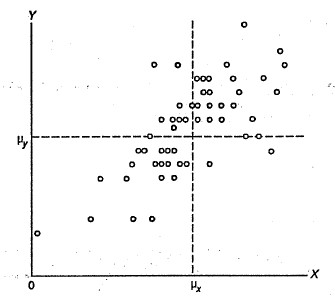
\includegraphics[height=2in]{pics/cov.jpg}
    \caption{An illustration of the covariance between two random variables}
    \label{fig:enter-label15}
\end{figure}

\subsubsection{Correlation}

The quantity
\begin{equation*}
    \rho_{XY}=\frac{\sigma_{XY}}{\sigma_{X}\sigma_{Y}}=\frac{Cov(X,Y)}{[Var(X)Var(Y)]^{1/2}}
\end{equation*}
is called the \textbf{correlation coefficient} between \(X\) and \(Y\). If \(Cov(X,Y)=0\) the \(Cor(X,Y)=0\), in which case \(X\) and \(Y\) are said to be \textbf{uncorrelated}. If \(X\) and \(Y\) are independent, then \(f_{XY}(x,y)=f_X(x)f_Y(y)\). From the definition of \(\sigma_{XY}\) that it is \(E_{XY}[(X-\mu_X)]E_{XY}[(Y-\mu_Y)]\). But \(E(X-\mu_X)=E(X)-\mu_X=0\). Hence, \(\sigma_{XY}=0 \text{ and } \rho_{XY}=0\) if two random variables are independent. \textbf{The converse need not be true}.

\begin{theorem}
    \begin{equation}
        |\rho_{XY}| \leq 1
    \end{equation}
\end{theorem}

\textbf{Proof:} Consider the random variable \((u-kv)^2\) where \(u\) and \(v\) are random variables and \(k\) is a real constant. Because \((u-kv)^2 \geq 0\), \(E[(u-kv)^2] \geq 0\). But
\begin{equation*}
    E[(u-kv)^2]=E(u^2)-2kE(uv)+k^2 E(v^2)
\end{equation*}

This quadratic in \(k\) must be greater than or equal to zero. To derive the necessary and sufficient condition for this, first define \(a=E(u^2)\), \(b=E(v^2)\) and \(h=E(uv)\). The quadratic can be written as follows:
\begin{equation*}
   a+2kh+k^2b = b \left[k-\frac{h}{b} \right]^2 + \frac{(ab-h^2)}{b}
\end{equation*}

The conditions \(b>0\) and \(ab-h^2 \geq 0\) are sufficient to make the quadratic nonnegative for all \(k\). They are also necessary. The required condition translates to
\begin{equation*}
    [E(uv)]^2 \leq E(u^2) E(v^2)
\end{equation*}
which is the Schwartz inequality. Let \(u=X-\mu_X\) and \(v=Y-\mu_Y\). Then
\begin{equation*}
    [Cov(X,Y)]^2 \leq Var(X)Var(Y)
\end{equation*}

If \(\rho_{XY}^2=1\), then \(E[(u-kv)^2]=0\) for some \(k\), implying that \(P(u=kv)=1\), that is, \(X-\mu_X=k(Y-\mu_Y)\). \(\rho_{XY}\) only measures \textbf{linear relationships} between the variables.

\subsection{Conditional Expectation}

\begin{definition}
    Let \(X\) and \(Y\) be continuous random variables and \(g(Y)\) be a continuous function. Then the \textbf{conditional expectation} of \(g(Y)\) given \((X=x)\), denoted by \(E_Y|X [g(Y)|X]\), is given by \(\int_{-\infty}^{\infty}g(y)f_Y|X(x,y)dy\), where \(f_Y|X(x,y)\) is the conditional density of \(Y\) given \(X\).
\end{definition}

\(E[g(Y)|X=x]\) is a function of \(x\) and not a random variable because \(x\) is fixed.

\begin{theorem}
    \textbf{Law of iterated expectations}.\\
    \begin{equation*}
        E_{XY}[g(Y)]=E_X[E_Y|X {g(Y)|X}]
    \end{equation*}
    that is, the unconditional expectation is the conditional expectation of conditional expectation
\end{theorem}

\textbf{Proof:} 
\begin{equation*}
    E_{XY}[g(Y)]=\int\int g(y) f_{XY}(x,y) dxdy    
\end{equation*}
But
\begin{equation*}
    f_{XY}(x,y)=f_Y|X(x,y)f_X(x)
\end{equation*}
Hence
\begin{equation*}
    E_{XY}[g(Y)]=\int\left[\int g(y)|f_Y|X(x,y)f_X(x)dx\right]
\end{equation*}
The expression in square brackets is the conditional expectation of \(g(Y)\) given \(X\). Therefore
\begin{equation*}
    E_{XY}[g(Y)]=\int E_Y|X[g(Y)|X] f_X(x)dx=E_X[E_Y|X\{g(Y)|X\}]
\end{equation*}

\subsection{Conditional Variance}

Let \(\mu_{Y|X}=E(Y|X)=\mu^*(X)\) be the conditional mean of \(Y\) given \(X\). Then the \textbf{conditional variance of \(Y\) given\(X\)} is defined as \(Var(Y|X)=E_{Y|X}[(Y-\mu)^2|X]\)

\begin{theorem}
    \(Var_{XY}=E_X[Var(Y|X]+Var_X(\mu^*)\), that is, the variance of \(Y\) is the mean of its conditional variance plus the variance of its conditional mean.
\end{theorem}

\textbf{Proof:} 
\begin{equation*}
    \begin{split}
        (Y-\mu_Y)^2=(Y-\mu^*+\mu^*-\mu_Y)^2 \\
        = (Y-\mu^*)^2+(\mu^*-\mu_Y)^2+2(Y-mu^*)(Y-\mu^*)\\
        E_{XY}(Y-\mu_Y)^2=E_X[E_{Y|X}(Y-\mu^*)^2|X]+E_X[E_{Y|X}(\mu^*-\mu_Y)^2|X]+2E_X[E_{Y|X}(Y-\mu^*)(Y-\mu_Y)|X]\\  
    \end{split}
\end{equation*}
The first term is \(E_X[Var(Y|X)]\), the second term is \(Var_X(\mu^*)\) because \(E_X(\mu^*)=\mu_Y\).The third term is zero because if \(X\) is given, \(\mu^*-\mu_Y\) is a constant and \(E_{Y|X}(Y-\mu^*)=0\).

\begin{theorem}
    \begin{equation*}
        Var(aX+bY)=a^2Var(X)+2ab Cov(X,Y) + b^2 Var(Y)
    \end{equation*}
\end{theorem}
\textbf{Proof:} 
\begin{equation*}
    \begin{split}
        E(aX+bY)=a \mu_X + b \mu_Y\\
        Var(aX+bY)=E[a(X-\mu_X)+b(Y-\mu_Y)]^2
    \end{split}
\end{equation*}
The expansion of this yields the result.

\subsubsection{Approximate Mean and Variance for \(g(X,Y)\)}

A linear approximation is obtained in the neighborhood of \((\mu_X,\mu_Y)\) as
\begin{equation*}
 g(X, Y) \approx g(\mu_X, \mu_Y) + \left( \frac{\partial g}{\partial X} \right)_* (X - \mu_X) + \left( \frac{\partial g}{\partial Y} \right)_* (Y - \mu_Y)
\end{equation*}
provided \(g(\mu_X,\mu_Y)\) and the two partial derivatives exist at the mean point \((\mu_X,\mu_Y)\),denoted by *. The mean and variance are
\begin{equation*}
    \begin{split}
        E[g(X,Y)] \approx g(\mu_X,\mu_Y)\\
        Var[g(X,Y)] \approx \sigma_X^2 \left( \frac{\partial g}{\partial X} \right)_* ^2 + \sigma_Y^2 \left( \frac{\partial g}{\partial Y} \right)_* ^2 + 2 \rho \sigma_X \sigma_Y \left( \frac{\partial g}{\partial X} \right)_* \left( \frac{\partial g}{\partial Y} \right)_*
    \end{split}
\end{equation*}

\subsection{The Bivariate Normal Distribution}

\begin{definition}
    Let \((X,Y)\) have the joint density
    \begin{equation*}
        f_{XY}(x,y)=\frac{1}{2 \pi \sigma_X \sigma_Y \sqrt{1-\rho^2}} \exp\left\{\frac{Q}{2(1-\rho^2)}\right\}
    \end{equation*}
    where 
    \begin{equation*}
    \begin{split}
        Q=\left(\frac{x-\mu_X}{\sigma_X}\right)^2-2\rho\frac{(x-\mu_X)(y-\mu_Y)}{\sigma_X\sigma_Y}+\left(\frac{y-\mu_Y}{\sigma_Y}\right)^2 \\
        -\infty<x<\infty,-\infty<y<\infty,-\infty<\mu_X<\infty,\infty<\mu_Y<\infty, \\
        \sigma_X,\sigma_Y>0, \text{ and } -1<\rho<1
    \end{split}
    \end{equation*}
    Then \((X,Y)\) is said to have the bivariate normal distribution.
\end{definition}

\begin{theorem}
    If \((X,Y)\) is bivariate normal, then the marginal distribution of \(X\) is \(N(\mu_X,\sigma_X^2)\) and that of \(Y\) is \(N(\mu_Y,\sigma_y^2)\)
\end{theorem}

\textbf{Proof:} We have \(f_X(x)=\int_{-\infty}^{\infty}f_{XY}(x,y)dy\). Let \(v=(y-\mu_Y)/\sigma_Y\). Then \(dy=\sigma_Y dv\). The marginal density of \(f_X(x)\) is therefore
\begin{equation*}
    \int_{-\infty}^{\infty} \frac{1}{2 \pi \sigma_X \sqrt{1-\rho^2}} \exp{\left[-\frac{(x-\mu_X)^2}{2\sigma_X^2(1-\rho)^2}+\frac{\rho(x-\mu_X)v}{\sigma_X(1-\rho^2)}-\frac{v^2}{2(1-\rho^2)} \right] dv}
\end{equation*}
By completing the square on \(v\), the expression in the square brackets becomes
\begin{equation*}
    -\frac{(x-\mu_X)^2}{2\sigma_X^2}-\frac{1}{2(1-\rho^2)}\left[v-\rho \frac{(x-\mu_X)}{\sigma_X} \right]^2
\end{equation*}
Let 
\begin{equation*}
    w=\frac{1}{\sqrt{(1-\rho^2)}}  \left[v-\rho \frac{(x-\mu_X)}{\sigma_X} \right]^2
\end{equation*}
Then \(dw=\frac{dv}{\sqrt{(1-\rho^2)}}\). Thus
\begin{equation*}
    f_X(x)= \int_{-\infty}^{\infty} \left[\frac{1}{\sigma_X\sqrt{2\pi}} e^{-\frac{(x-\mu_X)^2}{2 \sigma_X^2}} \frac{1}{\sqrt{2\pi}} e^{-\frac{w^2}{2}}\right]dw=\frac{1}{\sigma_X \sqrt{2\pi}} e^{-\frac{(x-\mu_X)^2}{2 \sigma_X^2}}
\end{equation*}
Because \(\int_{-\infty}^{\infty} e^{-w^2/2}=\sqrt{2\pi}\). \(X\) is thus a univariate normal with mean \(\mu_X\) and standard deviation \(\sigma_X\). \textit{The converse of the theorem need not be true}: that is, if the marginal distribution of \(X\) is univariate normal, the joint density between \(X\) and \(Y\) need not to be bivariate normal.

\begin{theorem}
    For a bivariate normal, the conditional density of \(Y\) given \(X=x\) is univariate normal with mean \(\mu_Y+(\rho \sigma_Y/\sigma_X)(x-\mu_X)\) and variance \(\sigma_Y^2(1-\rho^2)\). The conditional density of \(X\) given \(Y\) is also normal with mean \(\mu_X+(\rho \sigma_X/\sigma_Y)(y-\mu_Y)\) and variance \(\sigma_X^2(1-\rho^2)\)
\end{theorem}

\textbf{Proof:} \begin{equation*}
    f_{Y|X}(x,y)=\frac{f_{XY}(x,y)}{f_X(x)} = \frac{1}{\sigma_Y \sqrt{2\pi (1-\rho^2)}} \exp{-Q'/2}
    \end{equation*}
where
\begin{equation*}
    Q'=\frac{1}{1-\rho^2} \left[\frac{(y-\mu_Y)^2}{\sigma_Y^2} - 2\rho \frac{(y-\mu_Y)(x-\mu_X)}{\sigma_X \sigma_Y} + \frac{(x-\mu_X)^2}{\sigma_X^2} \right]-\frac{(x-\mu_X)^2}{\sigma_X^2}
\end{equation*}
which can be written as \([y-\mu_Y-(\rho \sigma_Y/\sigma_X)(x-\mu_X)]^2/\sigma_Y^2(1-\rho^2)\). The theorem follows directly from this.

The conditional expectation \(E(Y|X)\) is the regression of \(Y\) on \(X\). In the case of the bivariate normal density, this conditional expectation is of the form \(\alpha+\beta X\), where \(\alpha\) and \(\beta\) depend on the respective means, standard deviation and the correlation coefficient. This is the case of a simple linear regression in which the conditional expectation of a linear function of \(X\).

\subsection{Bivariate Transformations}

\begin{theorem}
    Let \(f_{XY}(x,y)\) be the joint density function of \(X\) and \(Y\) and \(U=g(X,Y), V=h(X,Y)\) be measurable transformations with the functions \(g\) and \(h\) being continuously differentiable. The the joint density function of \(U\) and \(V\) is given by
    \begin{equation*}
        f_{UV}(u,v)=f_{XY}[G(u,v),H(u,v)] \left| \frac{\partial(x,y)}{\partial(u,v)} \right|
    \end{equation*}
    provided the Jacobian of the transformation in non-vanishing and \(x=G(u,v)\), \(y=H(u,v)\) are the inverse transformations.
\end{theorem}

\textbf{Proof:} It's needed to express \(\int f_{UV}(u,v) dudv\) which is the probability density in a small area in the \((u,v)\) space in terms of the corresponding density in the \((x,y)\) space.

Consider the inverse mapping \(G\) and \(H\) that transforms the small rectangle in B into the parallelogram in A. The increments in \(x\) and \(y\) can be obtained by partial differentiation:

\begin{equation*}
\begin{split}
    dx=\frac{\partial x}{\partial u
    }du+\frac{\partial x}{\partial v} dv= a_{11}du+a_{12}dv\\
     dy=\frac{\partial y}{\partial u
    }du+\frac{\partial y}{\partial v} dv= a_{21}du+a_{22}dv
\end{split}
\end{equation*}

\begin{figure}
    \centering
    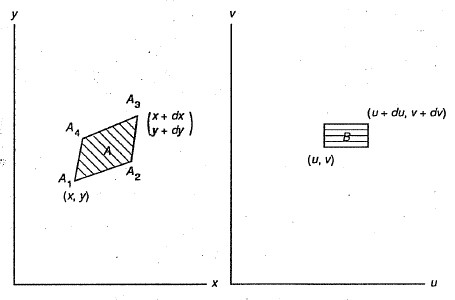
\includegraphics{pics/mapping.jpg}
    \caption{Mapping of the (X,Y) and (U,V) spaces}
    \label{fig:enter-label100}
\end{figure}

\begin{figure}
    \centering
    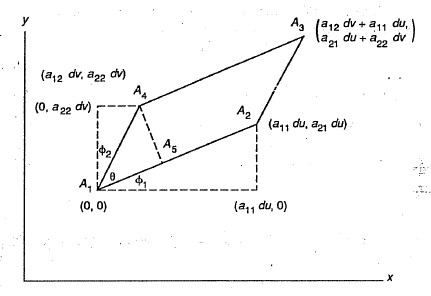
\includegraphics{pics/magnified.jpg}
    \caption{Magnified \(X,Y)\) space}
    \label{fig:enter-label391}
\end{figure}

Relative to the point \(A_1, A_2\) has coordinates \((a_{11}du,a_{21}du\) and \(A_4\) has coordinates \(a_{12}dv,a_{22}dv)\), obtained alternatively by setting \(du=0\) and \(dv=0\). \(A_3\) has coordinates \(a_{11}du+a_{12}dv, a_{21}du+a_{22}dv\); \(A_2\) and \(A_4\) have the indicated coordinates and hence \(A\) is a parallelogram.

We can draw a perpendicular line from \(A_4\) to \(A_2\) and denote as \(\phi_1, \phi_2 \text{ and } \theta\) the angles marked in the diagram.
\begin{equation*}
    Area(A)=(A_1 A_2)(A_4 A_5)=(A_1 A_2) (A_1 A_4) \sin \theta
\end{equation*}
Because \(\theta+\phi_1+\phi_2=\pi/2\), \(\sin\theta=\cos (\phi_1+\phi_2)=\cos \phi_1 \cos \phi_2-\sin \phi_1 \phi_2\)
\begin{equation*}
\begin{split}
    Area (A) = (A_1 A_2) (A_1 A_4) \cos[\phi_1+\phi_2] \\
    Area (A) = (A_1 A_2) (A_1 A_4) [\cos \phi_1 \cos \phi_2-\sin \phi_1 \sin \phi_2] \\
    Area (A) = (A_1 A_2 \cos \phi_1)(A_1 A_4\cos \phi_2)-(A_1 A_2 \sin \phi_1) (A_1 A_4 \sin \phi_2)\\
    Area (A) = a_{11}du .a_{22}dv-a_{21}du. a_{12}dv
\end{split}
\end{equation*}

Thus the area of parallelogram A becomes \(|J|dudv\), where \(J\) is the Jacobian of the transformation given by
\begin{equation*}
\begin{bmatrix}
    a_{11} & a_{12} \\
    a_{21} & a_{22}
\end{bmatrix}
=
\begin{bmatrix}
   \frac{\partial x}{\partial u} & \frac{\partial x}{\partial v} \\
    \frac{\partial y}{\partial u} & \frac{\partial y}{\partial v}  
\end{bmatrix}
= \frac{\partial (x,y)}{\partial(u,v)}
\end{equation*}

Using the area of \(A\) in \(P(A)\), we obtain
\begin{equation*}
    f_{UV}(u,v)=|J| f_{XY}(x,y)
\end{equation*}

The function \(f_{XY}(x,y)\) becomes \(f_{XY}[G(u,v),H(u,v)]\) by straightforward substitution. Therefore the joint density function of \((U,V)\) is 
\begin{equation*}
   f_{XY}[G(u,v),H(u,v)] \left|\frac{\partial (x,y)}{\partial (u,v)} \right|
\end{equation*}

In order to calculate the determinant of the Jacobian matrix, we can use the relation
\begin{equation*}
    \left|\frac{\partial (x,y)}{\partial (u,v)} \right|=\left|\frac{\partial (u,v)}{\partial (x,y)} \right|^{-1}
\end{equation*}
because the determinant of the inverse of a matrix is the reciprocal of the determinant of the matrix. The Jacobian of the inverse transformation is the inverse of the Jacobian of the direct transformation.

\subsection{The Convolution Formula}

A frequent application of the bivariate transformation is to obtain the distribution of the sum of two random variables. Thus, given that \(f_{XY}(x,y)\) is the joint density of \(X\) and \(Y\), we wish to find the density of the random variable \(X+Y\).

\begin{theorem}
    If \(f_{XY}(x,y)\) is the joint density of \(X\) and \(Y\), then the density of \(U=(X+Y)\) is
    \begin{equation*}
        f_U(u)=
        \begin{cases}
            \int f_{XY}(u-v,v)dv \hspace{0.5cm} \text{ continuous case} \\
            \sum_v f_{XY}(u-v,v) \hspace{0.5cm} \text{ discrete case}
        \end{cases}
    \end{equation*}
\end{theorem}
\textbf{Proof:} The trick is to use a dummy transformation \(V=Y\) along with the original one \(U=X+Y\). The Jacobian for this pair of transformations is
\begin{equation*}
    \frac{\partial(X,Y)}{\partial(U,V)} = 
    \begin{bmatrix}
        1 & -1 \\
        0 & 1
    \end{bmatrix}
    = 1
\end{equation*}
Therefore, \(f_{UV}(u,v)=f_{XY}(u-v,v)\). The density function of \(U\) is the marginal distribution of \((U,V)\). To obtain this, we have to sum or integrate the above over the \(v\) domain. Therefore,
\begin{equation*}
    f_U(u)=\int f_{XY}(u-v,v)dv \hspace{0.5cm} \text{ or } \hspace{0.5cm} \sum_v f_{XY}(u-v,v)
\end{equation*}

\subsection{Mixture Distributions}

In several applications of probability theory the distribution of random variables might depend on parameters or variables which themselves depend on other random variables. Example: we have a binomial random variable \(Y\) for which the probability of observing \(y\) successes out of \(n\) trials was \(\binom{n}{y}p^y(1-p)^{n-y}\). But \(p\) depends on another random variable \(X\) that followed an exponential distribution with parameter \(\theta\), more specifically, \(p=P(X \geq 500)\). Such a combination of distributions is called a \textbf{mixture distribution}. This might take the form \(f(x;\theta)\) where \(\theta\) depends on a random variable or the form \(f(x|y)\), where \(Y\) is another random variable.

Suppose \(f_{X|Y}(x,y)\) is the conditional density of \(X\) given that \(Y=y\). Let \(f_Y(y)\) be the marginal density of \(Y\). Then the joint density of \(X\) and \(Y\) is given by
\begin{equation*}
    f_{XY}(x,y)=f_{X|Y}(x,y)f_Y(y)
\end{equation*}

Our main interest, however, is in the marginal (that is unconditional) density of \(X\). For continuous random variables, this is obtained as
\begin{equation*}
    f_X(x)=\int f_{XY}(x,y)dy=\int f_{X|Y}(x,y) f_Y(y)dy
\end{equation*}

\subsection{Bivariate Characteristic Functions}

\begin{definition}
    The \textbf{joint characteristic function of} \((X,Y)\) is defined as
    \begin{equation*}
        \phi_{XY}(t_1,t_2)=E_{XY} \left[e^{i t_1 X+i t_2 Y} \right]
    \end{equation*}
    which, for a continuous pair of random variables, is
    \begin{equation*}
        \int_{-\infty}^{\infty} \int_{-\infty}^{\infty} e^{i t_1 X+i t_2 Y} f_{XY}(x,y) dx dy
    \end{equation*}
\end{definition}

\begin{theorem}
    The random variables \(X\) and \(Y\) are statistically independent if and only if their joint characteristic function is the product of the characteristic functions of the corresponding marginal distributions, that is, \(\phi_{XY}(t_1,t_2)=\phi_X(t_1)\phi_X(t_2)\).
\end{theorem}

\textbf{Proof:} If \(X\) and \(Y\) are independent,
\begin{equation*}
    \phi_{XY}(t_1,t_2)= \int_{-\infty}^{\infty} \int_{-\infty}^{\infty} e^{i t_1 X+i t_2 Y} f_X(x) f_Y(y) dxdy
\end{equation*}

We can integrate separately and get \(\phi_X(t_1)\phi_Y(t_2)\) on the right-hand side. 

\textbf{The converse is also true}. The characteristic function is unique in the multivariate case also.

\begin{theorem}
    The characteristic function of a bivariate normal is
    \begin{equation*}
        \phi_{XY}(t_1,t_2) =\exp{[it_1\mu_X+it_2\mu_Y-1/2(t_1^2\sigma_X^2+t_2^2\sigma_Y^2+2 \rho t_1 t_2 \sigma_X \sigma_Y)]}
    \end{equation*}
\end{theorem}

\begin{theorem}
    If \((X,Y)\) is bivariate normal, then \(U=aX+bY\) has the univariate normal distribution with mean \(a\mu_X+b\mu_Y\) and variance \(a^2\sigma_X^2+2ab\rho\sigma_X\sigma_Y+b^2\sigma_Y^2\)
\end{theorem}

\textbf{Proof:} \begin{equation*}
\begin{split}
    \phi_U(t)=E_{XY}(e^{iUt})=E_{XY}(e^{iaXt+ibYt}=\phi_{XY}(at,bt) \\
    = \exp{[it(a\mu_X+b\mu_Y)-1/2(a^2\sigma_X^2+2ab\rho \sigma_X \sigma_Y+b^2\sigma_Y^2)t^2]}
\end{split}
\end{equation*} 

\begin{theorem}
    If \(\phi_{XY}(t_1,t_2)\) is the characteristic function of \((X,Y)\), then the characteristic functions of the marginal distributions of \(X\) and \(Y\) are respectively \(\phi_{XY}(t,0)\) and \(\phi_{XY}(0,t)\).
\end{theorem}

\textbf{Proof:}
\begin{equation*}
\begin{split}
    \phi_X(t)=E_X(e^{iXt})= \int_{-\infty}^{\infty} e^{ixt}f_X(x) dx \\
    = \int_{-\infty}^{\infty} e^{ixt} \int_{-\infty}^{\infty} f_{XY}(x,y)dxdy=\phi_{XY}(t,0)
\end{split}
\end{equation*}

\begin{theorem}
    Let \(X\) and \(Y\) be random variables with joint characteristic function \(\phi_{XY}(t_1,t_2)\). Then \(X\) and \(Y\) are statistically independent if and only if \(\phi_{XY}(t_1,t_2)=\phi_{XY}(t_1,0) \phi_{XY}(0,t_2)\).
\end{theorem}

\begin{theorem}
    If \(\phi_X(t)\) and \(\phi_Y(t)\) are the characteristic functions of the two independent random variables \(X\) and \(Y\) respectively and \(\phi_{X+Y}(t)\) is the characteristic function of the random variable \(X+Y\), then \(\phi_{X+Y}(t)=\phi_X(t)\phi_Y(t)\)
\end{theorem}

\textit{The converse need not be true}.

\begin{theorem}
    If the assumptions of Theorem 4.10 hold, then
    \begin{equation*}
        \phi_{UV}(t_1,t_2)=E_{XY}[e^{it_1g(X,Y)+it_2h(X,Y)}]
    \end{equation*}
\end{theorem}

\textbf{Proof:} By definition, \(\phi_{UV}(t_1,t_2)=E_{UV}[e^{it_1U+it_2V]} = \int_U \int_V e^{it_1U+it_2V} f_{UV}(u,v) du dv\). In Theorem 4.10 we showed that \(f_{UV}(u,v)=f_{XY}|J|\) and that \(dxdy=|J|dudv\). With these, we carry out the integration over the \((X,Y)\) space.
\begin{equation*}
    \begin{split}
        \phi_{UV}(t_1,t_2)= \int_X \int_Y e^{it_1g(x,y)+it_2h(x,y)} f_{XY}(x,y) dxdy \\
        = E_{XY}[e^{it_1g(X,Y)+it_2h(x,y)}]
    \end{split}
\end{equation*}

\subsection{Multivariate Density Functions}

All the results derived for the bivariate case can be generalized no \(n\) random variables.

The joint density function of \(X_1,X_2,\dots,X_n\) will have the form \(f(x_1,x_2,\dots,x_n)\). If \(P(X_i<x_i \text{ for all } i)=F_X(x_1,\dots,x_n)\), then \(F\) is the CDF. If the \(X\)s are continuous random variables,
\begin{equation*}    f_X(x_1,x_2,\dots,x_n)=\frac{\partial^nF_X(x_1,x_2,\dots,x_n)}{\partial x_1\partial x_2\dots \partial x_n}
\end{equation*}

Expected values, marginal densities, and conditional densities are all defined similarly. If \(f(x_1,x_2,\dots,x_n)=\prod_i f_i(x_i)\), then the \(X\)s are independent by definition.

The multivariate characteristic function is \(\phi_X(t)=E_X(e^{it'X})\) where \(t\) is a column vector and \(X\) is a column vector of \(X\)s, both \(n \times 1\) and \(t'X=t_1X_1+t_2X_2+\dots+t_nX_n\) is the innerproduct. If the \(X\)s are independent, then \(\phi_X(t)=\prod_{i=1}^{i=n} \phi_{X_i}(t_i)\) and conversely. We have
\begin{equation*}
    \phi_{X_1+X_2+\dots+X_n}(t)=\prod_{i=1}^n \phi_{X_i}(t)
\end{equation*}
if all the \(X\)s are independent.

The general version of Theorem 4.10 is
\begin{equation*}
    f_U(u)=f_X[G(u)]\left|\frac{\partial x}{\partial u} \right|
\end{equation*}
in vector notation, or more completely, let the transformations be
\begin{equation*}
    \begin{split}
        U_1=g_1(X_1,X_2,\dots,X_n) \\
        U_2=g_2(X_1,X_2,\dots,X_n) \\
        \dots \dots \dots \dots \dots \dots \dots \dots\\
        U_n=g_n(X_1,X_2,\dots,X_n)
        \end{split}
\end{equation*}
and the inverse transformations be \(X_i=G_i(U_1,U_2,\dots,U_n)\). Then the joint density function \(f_U(u_1,\dots,u_n)\) is given by 
\begin{equation*}
f_X[G_1(u_1,u_2,\dots,u_n),G_2(u_1,u_2,\dots,u_n)\dots G_n(u_1,u_2,\dots,u_n)] |J|
\end{equation*}
where \(|J|=\left|\frac{\partial(x_1,x_2,\dots,x_n)}{\partial(u_1,u_2,\dots,u_n} \right|\).

The characteristic function of a marginal density can be obtained analogously to the bivariate case. For example
\begin{equation*}
    \phi_{X_1,X_2}(t_1,t_2)=\phi_X(t_1,t_2,0,0,\dots,0)
\end{equation*}

\subsection{The Multivariate Normal Distribution}

\begin{definition}
    Let \(X'=(X_1,X_2,\dots,X_n)\) be an n-dimensional vector random variable defined in $\mathbb{R}^n$ with a density function \(f_X(x)\), \(E(X_i)=\mu_i\) and \(\mu'=(\mu_1,\mu_2,\dots,\mu_n)\). Then the mean of the distribution is \(\mu=E(X)\) where \(\mu \text{ and } E(X)\) are \(n \times 1\) vectors, and hence \(E(X-\mu)=0\)
\end{definition}

\begin{definition}
    The covariance between \(X_i\) and \(X_j\) is defined as \(\sigma_{ij}=E[(X_i-\mu_i)(X_j-\mu_j)]\) where \(\mu_i=E(X_i)\). The matrix
    \begin{equation*}
    \Sigma = 
    \begin{bmatrix}
        \sigma_{11} & \sigma_{12} & \dots & \sigma_{1n} \\
        \sigma_{21} & \sigma_{22} & \dots & \sigma_{2n}
        \\ \vdots & \vdots & \ddots & \vdots \\
        \sigma_{n1} & \sigma_{n2} & \dots & \sigma_{nn}
    \end{bmatrix}
    \end{equation*}
also denoted as \(Var(X)\), is called the \textbf{covariance matrix of \(X\)}. In matrix notation, this can be expressed as \(\sum=E[(X-\mu)(X-\mu)']\) where \(X-\mu\) is \(n \times 1\). \emph{Diagonal elements are variances}.
\end{definition}

\newtheorem{property}{Property}[section]

\begin{property}
    If \( \underset{\substack{m \times 1}}{Y} =\underset{\substack{m \times n}}{A} \hspace{0.2cm} \underset{\substack n \times 1}{B} +\underset{\substack{n \times 1}}{b}\), then \(E(Y)=A\mu+b\)
\end{property}

\begin{property}
    $\Sigma$ is a symmetric positive semi-definite matrix
\end{property}

\textbf{Proof:} If \(c\) is a constant \(n \times 1\) vector,
\begin{equation*}
    \begin{split}
        Var(c'X)=E[(c'X-c'\mu)(c'X-c'\mu)']\\
        =E[(c'(X-\mu)(X-\mu')c)]=c' \Sigma c
    \end{split}
\end{equation*}

Because variance is a nonnegative number, this quadratic form is nonnegative for all \(c\), implying that \(\Sigma\) is positive semi-definite. If \(c'\Sigma c=0 \text{ for some $c$ }\), then \(Var(c'X)=0\), which implies linear dependence.

\begin{property}
    \(\Sigma\) is positive definite if and only if it is nonsingular.
\end{property}

\begin{property}
    \(\Sigma=E(XX')-\mu\mu'\).
\end{property}

\textbf{Proof:} 
\begin{equation*}
\begin{split}
    E(X-\mu)(X-\mu)'=E(XX'-\mu X'-\mu'X+\mu \mu') \\
    = E(XX')-E(X)\mu'-E(X')\mu+\mu \mu'= E(XX')-\mu \mu'
\end{split}    
\end{equation*}

\begin{property}
    If \(Y=AX+b\), then the covariance matrix of \(Y\) is \(A \Sigma A'\)
\end{property}

\textbf{Proof:} We have \(E(Y)=A\mu+b\). Hence
\begin{equation*}
    \begin{split}
        Var(Y)=E[(AX-A\mu)(AX-A\mu)'] = E[A(X-\mu)(X-mu)'A']\\
        = AE[(X-\mu)(X-\mu)']A' = A \Sigma A'
    \end{split}
\end{equation*}

\subsubsection{Approximate Mean and Covariance for \(g(X,Y)\)}

Let \(g_i(X)=g_i(X_1,X_2,\dots,X_n)\) for \(i=1,2,\dots,m\) be \(m\) measurable functions of the random vector $X$. The $n$ partial derivatives \(g_{ij}=\frac{\partial g_i}{\partial x_j}\) for \(j=1,2,\dots,n\) may be arranged as an \(n \times 1\) vector (call it \(q_i\)) so that
\begin{equation*}
    q_i'=\left[\frac{\partial g_i}{\partial x_1}, \frac{\partial g_i}{\partial x_2},\dots,\frac{\partial g_i}{\partial x_n} \right]
\end{equation*}

The generalization of the linear approximation to n-variate case is
\begin{equation*}
    g_i(X) \approx g_i(\mu)+\Sigma_{j=1}^{j=n} g_{ij}(X_j-\mu) = g_i(\mu) + q_i'(X-\mu)
\end{equation*}

An approximation to the expected value is given by \(E[g_i(X)] \approx g_i(\mu)\) or in vector notation, \(E[g(X)]=g(\mu)\). The approximate covariance matrix is \(Var[g(X]=Q \Sigma Q'\), where \(Q=[\partial g_i/\partial x_j]\) is the \(m \times n\) matrix of the partial derivatives \(\partial g_i/\partial x_j\).

\subsubsection{The Multivariate Normal Distribution}

Let \((X_1,X_2,\dots,X_n)\) be \(n\) independent random variables each of which is \(N(0,1)\). Then their joint density function is the product of individual density functions and is the \textbf{standard multivariate normal density}.
\begin{equation*}
    f_X(x)=f_X(x_1,x_2,\dots,x_n)=\left(\frac{1}{\sqrt{2\pi}} \right)^n e^{-\Sigma x_i^2/2}=\left(\frac{1}{2\pi}\right)^{n/2} e^{-x'x/2}
\end{equation*}

The corresponding characteristic function is \(e^{-\Sigma t_i^2/2}\) or \(e^{-t't/2}\).

Now make the linear transformation \(Y=AX+\mu\), where \(A\) and \(\mu\) are constant. By assumption, \(E(X)=0\) and \(E(XX')=I_n\).Therefore \(E(Y)=\mu\) and \(E[(Y-\mu)(Y-\mu)']=E[AXX'A']=AA'=\Sigma (say)\). Thus the vector \(Y\) has mean \(\mu\) and covariance matrix \(\Sigma\). Let \(A\) be nonsingular. The inverse transformation is \(X=A^{-1}(Y-\mu)\) and \(AA'=\Sigma\). To obtain the joint density, we need the Jacobian. But because the transformation is linear, the Jacobian is \(A^{-1}\) and its determinant is \(\frac{1}{|A|}\). The density function of \(Y\) is therefore
\begin{equation*}
\begin{split}
    f_Y(y)=\frac{1}{(2\pi)^{n/2}} |A|^{-1} \exp{\left[\frac{-(y-\mu)'(A^{-1})'A^{-1}(y-\mu)}{2} \right]}\\
    f_Y(y)=\frac{1}{(2\pi)^{n/2}|A|}  \exp{\left[\frac{-(y-\mu)'\Sigma^{-1}(y-\mu)}{2} \right]}
\end{split}    
\end{equation*}
because \(\Sigma=AA'\), and hence \(\Sigma^{-1}=(A')^{-1}A^{-1}\). Also, because \(|A'|=|A|\), \(|\Sigma|=(|A|)^2\), which means that \(|A|=|\Sigma|^{1/2}\). We thus have the density function of the \textbf{general multivariate normal distribution} \(N(\mu,\Sigma)\) as
\begin{equation*}
     f_Y(y)=\frac{1}{(2\pi)^{n/2}|\Sigma|^{1/2}}  \exp{\left[\frac{-(y-\mu)'\Sigma^{-1}(y-\mu)}{2} \right]}
\end{equation*}
where the mean vector of \(Y\) is \(\mu\) and the covariance matrix of \(Y\) is \(\Sigma\).

\subsubsection{Characteristic Function of \(N(\mu,\Sigma)\)}

\begin{equation*}
    \begin{split}
    \phi_Y(t)=E_X(e^{iY't})=E_X(e^{i(AX+\mu)'t})=e^{i \mu't}E_X(e^{iX'A't})\\
    =e^{i\mu't}\phi_X(A't)=e{i\mu't}\exp{-[(A't)'(A't)/2]}
    \end{split}
\end{equation*}
Noting that \(AA'=\Sigma\), we have \(\phi_Y(t)=\exp{[i\mu't-(t'\Sigma t/2)]}\)

\begin{property}
    If \(Y\) is multivariate normal, then \(Y_1,Y_2,\dots,Y_n\) will be independent if and only if \(\Sigma\) is diagonal.
\end{property}

\begin{property}
    A linear combination of multivariate normal random variables is also multivariate normal. Let \(Y\sim N(\mu,\Sigma)\). Then \(Z=AY \sim N(A\mu,A\Sigma A')\), where \(A\) is an \(n \times n\) matrix.
\end{property}

\textbf{Proof:} 
\begin{equation*}
    \phi_Z(t)=E(e^{iZ't})=E(e^{iY'A't})=\phi_Y(A't)=\phi_Y(t)=\exp{[i\mu'A't-(t'A\Sigma A' t/2)]}
\end{equation*}
which is the characteristic function of \(N(A\mu,A\Sigma A')\).

\begin{property}
    If \(Y\sim(\mu,\Sigma)\) and \(\Sigma\) has rank \(k<n\), then there exists a nonsingular \(k \times n\) matrix \(A\) such that the \(k \times 1\) matrix \(X=[A^{-1}O](Y-\mu)\) is a \(k\)-variate normal with zero mean and covariance matrix \(I_k\), where \(O\) is a \(k \times (n-k)\) matrix of zeros.
\end{property}

\textbf{Proof:} If \(\Sigma\) has rank \(k\), there exists a nonsingular matrix \(A\) such that \(AA'\) is a submatrix of \(\Sigma\) that is nonsingular. It is easy to verify from the previous property that \(X\sim N(0,I_k)\)


\subsubsection{Marginal and Conditional Distributions of \(N(\mu,\Sigma)\)}

Let \(Y\sim N(\mu,\Sigma)\), and consider the following partition:
\begin{equation*}
    Y=\begin{bmatrix}
        Y_1\\
        Y_2
    \end{bmatrix}
    ; \mu = \begin{bmatrix}
        \mu_1\\
        \mu_2
    \end{bmatrix}
    ; \Sigma = \begin{bmatrix}
        \Sigma_{11} & \Sigma_{12}\\
        \Sigma_{21} & \Sigma_{22}
    \end{bmatrix}
\end{equation*}
where the \(n\) random variables are partitioned into \(n_1\) and \(n_2\) variates (\(n_1+n_2=n\)).

\begin{theorem}
    Given the above partition, the marginal distribution of \(Y_1\) is \(N(\mu_1,\Sigma_{11})\) and the conditional density of \(Y_2\) given \(Y_1\) is multivariate normal with mean \(\mu_2+\Sigma_{21}\Sigma_{11}^{-1}(Y_1-\mu_1)\) and covariance matrix \(\Sigma_{22}-\Sigma_{21}\Sigma_{11}^{-1}\Sigma_{12}\).
\end{theorem}

\begin{lemma}
    The partitioned inverse of \(\Sigma\) can be written as follows:
    \begin{equation*}
        \Sigma^{-1}=\begin{bmatrix}
            \Sigma_{11}^{-1}+FEF',-FE\\
            -EF',E
        \end{bmatrix}
        = \begin{bmatrix}
            \Sigma_{11}^{-1} & 0\\
            0 & 0
        \end{bmatrix}
        + \begin{bmatrix}
            -F\\
            I_{n_2}
        \end{bmatrix}
        E [-F', I_n]
    \end{equation*},
    where \(F=\Sigma_{11}^{-1}\Sigma_{12}\) and \(E=(\Sigma_{22}-\Sigma_{21}\Sigma_{11}^{-1}\Sigma_{12})^{-1}\)
\end{lemma}

\begin{lemma}
    \begin{equation*}
        |\Sigma|=|\Sigma_{11}|.|E^{-1}|
    \end{equation*}
\end{lemma}

\textbf{Proof:} Consider the quadratic for \(Q=(Y-\mu)'\Sigma^{-1}(Y-\mu)\). Using Lemma 4.1 it can be written as
\begin{equation*}
    Q = [(Y_1-\mu_1)',(Y_2-\mu_2)'] \begin{bmatrix}
        \Sigma_{11}^{-1} & 0 \\
        0 & 0 
    \end{bmatrix}
    \begin{bmatrix}
        Y_1-\mu_1\\
        Y_2-\mu_2
    \end{bmatrix}
    + [(Y_1-\mu_1)',(Y_2-\mu_2)'] \begin{bmatrix}
        -F\\
        I_{n_2}
    \end{bmatrix}
    E [F',I_{n_2}] \begin{bmatrix}
        Y_1-\mu_1\\
        Y_2-\mu_2
    \end{bmatrix}
\end{equation*}

Expanding these we obtain

\begin{equation*}
    Q= (Y_1-\mu_1)' \Sigma_{11}^{-1} (Y_1-\mu_1)+[(Y_2-\mu_2)-F'(Y_1-\mu_1)]'E[Y_2-\mu_2-F'(Y_1-\mu_1)]
\end{equation*}

Call the first term \(Q_1\) and the second \(Q_2\). The joint density of \((Y_1,Y_2)\) is
\begin{equation*}
    f_Y(y_1,y_2)=\frac{1}{(2\pi)^{n/2}|\Sigma|^{1/2}} \exp{[-Q/2]}
\end{equation*}

From Lemma 4.2,

\begin{equation*}
    |\Sigma|^{1/2}|=|\Sigma_{11}|^{1/2} |E|^{-1/2}|
\end{equation*}

Hence \(f_Y(y_1,y_2)\) can be re written as follows:
\begin{equation*}
    \frac{1}{(2\pi)^{n_1/2}|\Sigma_{11}|^{1/2}} \exp{[-Q_1/2]} \frac{1}{(2\pi)^{n_2/2}|E|^{-1/2}} \exp{[-Q_2/2]} = f_{Y_1}(y_1) f_{Y_2|Y_1}(y_1,y_2)
\end{equation*}

Note that the first part involves only \(Y_1\) and \(\Sigma_{11}\). If you fix \(Y_1\) in the second part, it has the form of the multivariate normal density of \(Y_2\) for a given \(Y_1\), which integrates to 1 with respect to \(Y_2\). The first part is therefore the marginal density of \(Y_1\). Both are multivariate normal. Hence
\begin{equation*}
\begin{split}
        Y_1 \sim N(\mu_1,\Sigma_{11})\\
        Y_2|Y_1 \sim N[\mu_2+F'(Y_1-\mu_1),E^{-1}]
\end{split}
\end{equation*}

Because \(F=\Sigma_{11}^{-1}\Sigma_{22}\) and \(E^{-1}=\Sigma_{22}-\Sigma_{21}\Sigma_{11}^{-1}\Sigma_{12}\), we have
\begin{equation*}
     Y_2|Y_1 \sim N[\mu_2+\Sigma_{11}^{-1}\Sigma_{22}(Y_1-\mu_1),\Sigma_{22}-\Sigma_{21}\Sigma_{11}^{-1}\Sigma_{12}]
\end{equation*}

\subsection{The Chi-Square Distribution}

The \textbf{chi-square distribution} is a special case of the gamma distribution. The density function for gamma is
\begin{equation*}
    f_X(x)=\frac{1}{\beta^{\alpha}\Gamma(\alpha)}x^{\alpha-1}e^{-(x/\beta)}, \hspace{0.5cm} x>0, \hspace{0.2cm} \alpha,\beta>0
\end{equation*}
where \(\Gamma(\alpha)\) is the gamma function \(\int_0^{\infty}y_{\alpha-1}e^{-y}dy \text{ for } \alpha>0\). In the special case where \(\alpha=n/2 \text{ and } \beta=2\), the density function is
\begin{equation*}
    f_X(x)=\frac{(x/2)^{(n/2)-1}e^{-(x/2)}}{2 \Gamma(n/2)} \hspace{0.5cm} x>0
\end{equation*}
the distribution is a \textbf{chi-square distribution with $n$ degrees of freedom and is written as} \(\chi_n^{2}\).

An even more special case arises when the degree of freedom is 1. It is easily shown that if \(X\sim N(0,1)\), then \(Y=Z^2\sim\chi_1^2\). Thus the square of a standard normal is chi-square with 1 degree of freedom. The distribution of \(Y\) is
\begin{equation*}
\begin{split}
    F_Y(y)=P(Y \leq y) = P(Z^2 \leq y) = P(-\sqrt{y} \leq Z \leq \sqrt{y}) \\
    = 2P(Z \leq \sqrt{y})=2 F_Z(\sqrt{y})
\end{split}
\end{equation*}
because of the symmetry of \(N(0,1)\) around the origin. The density function is
\begin{equation*}
\begin{split}
    f_Y(y)=\frac{dF_y(y)}{dy}=2F_Z'(\sqrt{y})\frac{1}{2\sqrt{y}} \\
    = \frac{1}{\sqrt{y}}f_Z(\sqrt{y})=\frac{1}{2\pi}y^{-1/2}e^{-y/2} 
\end{split}
\end{equation*}

This can be written as
\begin{equation*}
    f_Y(y)=\frac{1}{2\sqrt{\pi}} (y/2)^{-1/2}e^{-y/2} = \frac{1}{2\Gamma(1/2)} (y/2)^{-1/2}e^{-y/2}
\end{equation*}
which is the same as the density of \(\chi_1^2\).

\begin{theorem}
    The characteristic function of \(\chi_n^2\) is \((1-2it)^{-n/2}\).
\end{theorem}

\textbf{Proof:} Using the density function given above, we have
\begin{equation*}
    \begin{split}
        \phi(t)=\int_0^{\infty} \frac{(x/2)^{(n/2)-1}e^{-(x/2)}}{2 \Gamma(n/2)} e^{ixt} dx \\
        = \int_0^{\infty} \frac{(x/2)^{(n/2)-1}e^{-x(1-2it)/2)}}{2 \Gamma(n/2)} dx
    \end{split}
\end{equation*}
Define \(y=x(1-2it)\). Thus the above integral becomes
\begin{equation*}
    \phi(t)=\left[ \int_0^{\infty} \frac{(y/2)^{(n/2)-1}e^{-y/2)}}{2 \Gamma(n/2)} dy \right] (1-2it)^{-n/2}
\end{equation*}

But the expression in the square brackets is 1 because the integrand is the density for \(\chi_1^2\). Therefore \(\phi(t)=(1-2it)^{-n/2}\)

\textbf{Corollary}. The chi-square distribution has the \textbf{additive property}, that is, if \(X\sim\chi_m^2\), \(Y\sim\chi_n^2\), and \(X\) and \(Y\) are independent, then their sum \(X+Y\sim\chi_{n+m}^2\). Thus the sum of independent chi-square is also chi-square with d.f as the sum of the d.f.

\textbf{Proof:} The characteristic function of the sum of independent random variables is the product of their characteristic functions. Therefore
\begin{equation*}
    \begin{split}
        \phi_{X+Y}(t)=\phi_X(t)\phi_Y(t)=(1-2it)^{-m/2} (1-2it)^{-n/2}\\
        = (1-2it)^{-(m+n)/2}
    \end{split}
\end{equation*}
which is the characteristic function of a chi-square distribution with \(m+n\) d.f.

\begin{theorem}
    Let \(Z_1, Z_2,\dots,Z_n)\) be independently and identically distributed as \(N(0,1)\). Then the distribution of \(X=\sum Z_i^2\) is \(\chi_n^2\). Thus the distribution of the sum of squares of \(n\) independent standard normal random variables is \(\chi_n^2\).
\end{theorem}

\textbf{Proof:} Since \(Z_i \text{ is } N(0,1), Y_i=Z_i^2 \text{ is } \chi_1^2\). It follows from the additive property that \(X=\sum Y_i=\sum Z_i^2\) is \(\chi_n^2\).

\begin{theorem}
    If \(X_i\sim(\mu_i,\sigma_i^2),i=1,2,\dots,n\) and \(X_1,X_2,\dots,X_n\) are all independent, then \(Y=\sum_{i=1}^{i=n}[(X_i-\mu_i)/\sigma_i]^2\) has the chi-square distribution with \(n\) d.f.
\end{theorem}

\textbf{Proof:} Let \(Z_i=(X_i-\mu_i)/\sigma_i\). Then \(Z_i\sim(0,1)\) for all \(i\) and are all independent. Hence by the previous theorem, \(\sum Z_i^2\sim\chi_n^2\).

\subsubsection{Mean and variance of Chi-square}

We take the derivative of \(\phi(t)\) once and evaluate it at \(t=0\). This will equal \(i\) times the mean.
\begin{equation*}
    \begin{split}
        \phi'(t)=\frac{-n}{2}(1-2it)^{(-n/2)-1}(-2i)\\
        \phi'(0)=\frac{-n}{2} (-2i) = ni = \mu_1'i
    \end{split}
\end{equation*}

Hence the mean is \(n\). To get the second moment we need \(\phi''(0)\).
\begin{equation*}
    \begin{split}
        \phi''(t)=\frac{-n}{2} \left(\frac{-n}{2}-1\right)(1-2it)^{(-n/2)-2}(-2i)^2\\
        \phi''(0)=i^2\mu_2'=i^2n(n+2)
    \end{split}
\end{equation*}

Hence the second moment, \(\mu_2'=n(n+2)\).
\begin{equation*}
    \sigma^2=\mu_2'-(\mu_1')^2=n(n+2)-n^2=2n
\end{equation*}

Therefore the \(\chi_n^2\) distribution has mean \(n\) and variance \(2n\).

\subsection{Distributions of Quadratic Forms}

\begin{theorem}
    Let \(Y\sim N_n(\mu,\Sigma)\). Then the quadratic form \((Y-\mu)'\Sigma(Y-\mu)\sim\chi_n^2\) where \(n=rank(\Sigma)\) and is the number of \(Y\)'s.
\end{theorem}

\textbf{Proof:} Because \(\Sigma\) is a positive definite matrix, there exists a nonsingular matrix \(A\) such that \(AA'=\Sigma\). Now define the new random variable \(X=A^{-1}(Y-\mu)\). Because \(X\) is a linear combination of the \(Y\)'s, \(X\) is also multivariate normal.
\begin{equation*}
    \begin{split}
        E(X)=A^{-1}E(Y-\mu)=0\\
        E(XX')=A^{-1}E[(Y-\mu)(Y-\mu')](A^{-1})'=A^{-1}AA'(A')^{-1}=I_n
    \end{split}
\end{equation*}
\((A^{-1})'=(A')^{-1}\). Hence the \(X\)s are all independent and distributed as \(N(0,1)\). Thus, by theorem, \(X'X\sim\chi_n^2\). But
\begin{equation*}
    X'X=(Y-\mu)'(A^{-1})'A^{-1}(Y-\mu)=(Y-\mu)'\Sigma^{-1}(Y-\mu)
\end{equation*}
Hence \((Y-\mu)'\Sigma^{-1}(Y-\mu)\sim\chi_n^2\).

\begin{theorem}
    Let \(X\sim N_n(0,I_n)\) and \(A\) be a\(n \times n\) symmetric matrix of rank \(k<n\). Then \(X'AX\sim\chi_k^2\) if and only if \(A\) is idempotent.
\end{theorem}

\textbf{Proof:} Because \(A\) is a symmetric matrix, there exists a nonsingular orthogonal matrix \(C\) (for which \(CC'=I)\) such that \(C'AC\) is diagonal and the elements are the characteristic roots \(\lambda_i\). Now let \(Y=C'X\). Then \(X=CY\) and \(X'AX=Y'C'ACY=\sum_i \lambda_i Y_i^2\). Thus \(X'AX\sim\chi_k^2\) if and only if \(k\) of the \(\lambda\)s are equal to 1 and the others are zero, that is, if \(A\) is idempotent.

\begin{theorem}
    Let \(Y\sim N_n(0,\Sigma)\) and \(A\) be \(n \times n\) and symmetric with rank \(k<n\). Then \(Y'AY\sim\chi_k^2\) if and only if \(A\Sigma A=A\).
\end{theorem}

\textbf{Proof:} Let \(\Sigma^{1/2}\) be the square root of \(\Sigma\). Define \(X=\Sigma^{-1/2}Y\). Then \(X\sim N(_n(0,1)- YA'Y=X'\Sigma^{1/2}A^Sigma^{1/2}X\). This has a \(\chi_k^2\) distribution if and only if \(\Sigma^{1/2}A\Sigma^{1/2}\).
\begin{equation*}
    \Sigma^{1/2}A\Sigma^{1/2}.\Sigma^{1/2}A \Sigma^{1/2}=\Sigma^{1/2}A\Sigma^{1/2}
\end{equation*}

Pre and post multiplying both sides by \(\Sigma^{1/2}\) we get \(A\Sigma A=A\)

\begin{theorem}
    Let \(X\sim N_n(0,I_n)\) and \(A \text{ be } n \times n\). Then the characteristic function of \(X'AX \text{ is } |I-2itA|^{-1/2}\).
\end{theorem}

\textbf{Proof:}
\begin{equation*}
    \begin{split}
        \phi_{X'AX}(t)=E_X[e^{itx'Ax}]=\frac{1}{(2\pi)^{n/2}} \int e^{itx'Ax} e^{-x'x/2} dx\\
        =\frac{1}{(2\pi)^{n/2}} \int e^{-x'(I-2itA)x/2} dx\\
        =|I-2itA|^{-1/2} \left[\frac{1}{(2\pi)^{n/2}} \frac{1}{|I-2itA|^{1/2}} \int e^{-x'(I-2itA)x/2} dx \right]       
    \end{split}
\end{equation*}

But the expression in square brackets is the multivariate normal density with mean 0 and \(\Sigma^{-1}=(I-2itA)\). As \(N(0,\Sigma)\) should integrate to 1, the above expression becomes \(|I-2itA|^{-1/2}\).

\begin{theorem}
    If \(X\sim N_n(0,I)\), then the quadratic forms \(X'A_1X \text{ and } X'A_2X\) are independent if and only if \(A_1A_2=0\)
\end{theorem}

\textbf{Proof:} \(U=X'A_1X\) has the characteristic function \(|I-2itA_1|^{-1/2},V=X'A_2X\) has the characteristic function \(|I-2itA_2|^{-1/2}\) and \(U+V=X'(A_1+A_2)X\) has the characteristic function \(|I-2it(A_1+A_2)|^{-1/2}\). If \(U \text{ and } V\) are independent, then \(\phi_{U+V}(t)=\phi_U(t)\phi_V(t)\). This implies that
\begin{equation*}
    |I-2it(A_1+A_2)|=|I-2itA_1||I-2itA_2|
\end{equation*}

Because \(|A||B|=|AB| \text{ when } A \text{ and } B \text{ are } n \times n\), the right-hand side becomes \(|I-2it(A_1+A_2)+4i^2t^2A_1A_2|\). We note that the left and right sides will be equal if and only if \(A_1A_2=0\). Thus the independence of \(U \text{ and } V\) implies \(A_1A_2=0\).

To prove that \(A_1A_2=0\) implies the independence of \(U \text{ and } V\), note that
\begin{equation*}
    \begin{split}
        \phi_{UV}(t_1,t_2)=E \left[e^{it_1U+it_2V} \right]=k \int e^{it_1x'A_1x+i t_2 x'A_2x-(x'x/2)} dx\\
        = k \int e^{-x'(I-2it_1A_2-2it_2A_2)x} dx\\
        = |I-2it_1A_2-2it_2A_2|^{-1/2}=\phi_U(t_1)\phi_V(t_2)
    \end{split}
\end{equation*}

Because \(A_1A_2=0\). Hence \(U \text{ and } V\) are independent

\begin{theorem}
    If \(X\sim N_n(0,I)\) and \(A\) is an idempotent matrix of order \(n\), then the quadratic form \(X'AX\) and the linear form \(n'X\) are independent if \(Ab=0\).
\end{theorem}

\textbf{Proof:} The quadratic form \(X'AX\) can be written as \((AX)'(AX)\). Also, the covariance matrix between \(AX \text{ and } b'X \text{ is } E(AXX'b)=0 \text{ because } Ab=0\). Because \(AX \text{ and } b'X\) are linear functions of normal variates that have zero covariances, they are also independent. It follows from this that \(b'X\) is independent of a function of \(AX\), in particular, independent pf \(X'AX\).

\begin{theorem}
    If \(X\sim N(0,I_n)\) and \(A_1 \text{ and } A_2\) are \(n \times n\) matrices of rank \(k_1 \text{ and } k_2\) respectively, then \(X'A_1X \text{ and } X'A_2X\) are independent chi-square variates if \(A_1A_2=0\) and \(A_2\) and \(A_2\) are both idempotent.
\end{theorem}

\textbf{Proof:} From previous theorems.

\textbf{Corollary:} the necessary and sufficient conditions for the previous Theorem to hold when \(X\sim N(0,\Sigma)\) are \(A_1\Sigma A_2=A_1, A_2 \Sigma A_2=A_2\), and \(A_1\Sigma A_2=0\).

\textbf{Proof:} Make the transformation \(Y=\Sigma^{-1/2}X\). Then \(Y\) is distributed as \(N(0,I_n)\). The condition \(A_1 \Sigma A_2=0\) follows from the previous Theorem and the other, from 25.
\subsection{Multinomial Distributions}

In a Bernoulli trial, an experiment has exactly two outcomes. Some may have more than two. Suppose in a given trial, one of \(k\) mutually exclusive events must occur (\(A_1,A_2,\dots,A_k\)). Let \(P(A_i)=P_i\) and define the random variable \(Y_i\), which takes value 1 if \(A_i\) occurs and 0 otherwise. Thus \(P(Y_i=1)=P_i\). The joint density of the \(Y\)s can be written as
\begin{equation*}
    f(y_1,y_2,\dots,y_n)=P_1^{y_1}P_2^{y_2}\dots P_k^{y_k}
\end{equation*}
which is a discrete random variable called the \textbf{multinomial distribution}.

\subsubsection{The Multinomial Logit}

A special type of the multinomial distribution commonly used is the \textbf{multinomial logit} for which \(P_i\) is conditioned on one or more random variables \(X\) and the functional form is the logistic function. In particular,
\begin{equation*}
    P_i=\frac{e^{x_i \theta}}{\sum_{j=1}^{j=k}e^{x_j \theta}}
\end{equation*}

If a cumulative normal distribution is used instead of the logistic, we have a \textbf{multinomial probit}.

\section{Sampling Theory}

The probability model consists of a probability space represented by the triple \((S,\mathcal{F},P)\) and a random variable \(X\) represented by the family of density functions \(f(x;\theta)\), where \(x\) is a particular value that \(X\) can take, and \(\theta\) are parameters belonging to the parameter space \(\Theta\). The totality of elements about which some information is desired is called a \textbf{population}.

In probability theory, we assume that the density function is either known or can be derived from some fundamental principle. The actual values of the parameters underlying the identified family of distributions are unknown, however, and have to be estimated in some way.

\textbf{Statistical inference} is the subject that deals with the problems associated with the estimation of the unknown parameters underlying statistical distributions, measuring their precision, testing hypotheses on them, using them in generating forecasts and so forth. An investigator often resorts to measuring attributes for a small portion of the population known as \textbf{sample}.

\subsection{Independent,dependent and random samples}

The observations on a random variable \(X\) are denoted by  \(x_1,x_2,\dots,x_n\) where \(n\) is the number of observations. These are thus realizations of an experiment repeated \(n\) times. Observations will \(x_{ij} \text{ for } i=1,2,\dots,k, j=1,2,\dots,n\).

Although an observation is simply a measured attribute, conceptually it can be treated as a random variable because of the uncertainty in its value.

\subsubsection{Independent Sample}

\begin{definition}
    The observations \(x_1,x_2,\dots,x_n\) are said to form an \textbf{independent sample} if the joint density function of the \(x_i\)'s has the form
    \begin{equation*}
        f_X(x_1,x_2,\dots,x_n)=\prod_{i=1}{i=n} f_{X_i}(x_i;\theta_i)
    \end{equation*}

Because \(f_{X_i}\) might be different across \(i\), here we are not assuming that the \(x\)'s have the same distribution.
\end{definition}

\subsubsection{Random Sample}

\begin{definition}
    A \textbf{random sample} from the a population is a set of independent, identically distributed random variables \(x_1,x_2,\dots,x_n\), each of which has the same distribution as \(X\).
\end{definition}

The joint density of \(x_1,x_2,\dots,x_n\) is simply the product of individual densities. Thus, if \(f(x)\) is the common density function of the \(X_i\)'s, then

\begin{equation*}
    f_X(x_1,x_2,\dots,x_n)=f(x_1)f(x_2)\dots(x_n)=\prod_{i=1}^{i=n} f(x_i)
\end{equation*}

\subsubsection{Dependent Sample}

Suppose the observations obtained on the random variable \(X\) are over time. The assumption of independence of observations between years is not likely to hold. In this case we have \textbf{dependent sample}. The joint density \(f_X(x_1,x_2,\dots,x_n; \theta)\) can be factored as follows
\begin{equation*}
    f(x_n|x_1,x_2,\dots,x_{n-1};\theta) f(x_1,x_2,\dots,x_{n-1};\theta)
\end{equation*}

Repeated use of this decomposition yields the following expression for the joint density:
\begin{equation*}
    f(x_1,x_2,\dots,x_n;\theta)=\prod_{i=1}^{i=n} f(x_i|x_1,x_2,\dots,x_{i-1};\theta)
\end{equation*}

\subsection{Sample Statistic}

\begin{definition}
    A \textbf{statistic} is a function of the observable random variable(s) that doesn't contain any unknown parameters.
\end{definition}

Examples:
\begin{equation*}
    \begin{split}
       \text{Sample variance } s^2=\frac{\sum_{i=1}^{i=n}(x_i-\overline{x})^2}{n-1} \\
       \text{Sample moments: } m_r=\frac{1}{n} \sum_{i=1}^{i=n}x_i^r \\
       \text{Sample correlation: } s_{xy}=\frac{1}{n-1} \sum_i(x_i - \overline{x})(y_i-\overline{y})\\
       \text{Sample correlation coefficient: } r_{xy}=\frac{s_{xy}}{s_x s_y} = \frac{\sum(x_i-\overline{x})(y_i-\overline{y})}{[\sum (x_i-\overline{x})^2]^{1/2} [\sum(y_i-\overline{y})^2]^{1/2}} 
    \end{split}
\end{equation*}

\begin{theorem}
    If \(x_1,x_2,\dots,x_n\) is a random sample from a population with mean \(\mu\) and variance \(\sigma^2\) and all the \(c_i\)'s are constant, then
    \begin{equation*}
        Y=c_1x_1+c_2x_2+\dots+c_nx_n=c'x
    \end{equation*}
    has the following expectation and variance.
    \begin{equation*}
        \begin{split}
            E(Y)=\mu (\sum c_i) = (c_1+c_2+\dots+c_n) \mu \\
            Var(Y)=\sigma^2(c_1^2+c_2^2+\dots+c_n^2)=\sigma^2c'c
        \end{split}
    \end{equation*}
\end{theorem}
\textit{Corollary:}
\begin{equation*}
    E(\overline{x})=\mu; \hspace{0.5cm} Var(\overline{x})=\sigma^2/n
\end{equation*}

\textbf{Proof:} \begin{equation*}
    \begin{split}
        E(Y)=E(\sum_i c_ix_i)=\sum c_i E(x_i)=\mu(\sum c_i)\\
        Var(Y)=E[(Y-E(Y)]^2=E[\sum c_i(x_i-\mu)]^2\\
        = E\left[\sum c_i^2(x_i-\mu)^2\right]+\sum_{i \neq j} \sum c_i c_j E[(x_i-\mu)(x_j-\mu)]\\
        \text{ But because the } x's \text{ are independent,}\\
        Cov(x_i,x_j)=E[(x_i-\mu)(x_j-\mu)]=0\\
        \text{ for all } i \neq j. \text{ The corollary follows by setting } c_i=1/2 \text{ for all } i. 
    \end{split}
\end{equation*}

Thus the expected value of the mean of a sample is the mean of the population. Furthermore, \(E(m_r)=\mu_r'\)

\subsection{Sampling Distributions}

Because a sample statistic if a function of random variables, it has a statistical distribution. This is called the \textbf{sampling distribution} of the statistic.

As an example, suppose \(x_1,x_2,\dots,x_n\) are iid as \(N(\mu,\sigma^2)\). Then because linear combinations of normal variates are also normally distributed, then \(\overline{x}\sim N(\mu,\sigma^/n)\) or equivalently the standardized version \(s=\sqrt{n} (\overline{x}-\mu)\sigma\sim N(0,1)\). Thus the sampling distribution of the mean is normal with the same mean but a much smaller variance.

\subsubsection{Distribution of the Sample Variance of a Normal Variate}

\begin{theorem}
    Let \(x_1,x_2,\dots,x_n\) be a random sample from \(N(0,1)\). Then
    \begin{itemize}
        \item[a)] \(\sum_{i=1}^{i=n}(x_i-\overline{x})^2\) has the chi-square distribution with \(n-1\) d.f.
        \item[b)] \(\overline{x}\) has the normal distribution\((0,1/n)\).
        \item[c)] \(\overline{x}\) and \(\sum(x_i-\overline{x})^2\) are statistically independent.
    \end{itemize}
\end{theorem}

\textbf{Proof:} Let \(u=n\overline{x}^2 \text{ and } v=\sum(x_i-\overline{x})^2\). Then we have
\begin{equation*}
    u=n\left(\sum x_i\right)^2/n^2=(1/n)\left(\sum_i x_i^2+\sum_i \sum_{\neq j} x_i x_j \right)
\end{equation*}
This can be expressed as the quadratic for \(x'A_1 x_1\), where
\begin{equation*}
A_1=\frac{1}{n}
    \begin{bmatrix}
        1 & 1 & . & . & . & . & . & 1\\
        1 & 1 & . & . & . & . & . & 1\\
        . & . & . & . & . & . & . & 1\\
        1 & 1 & . & . & . & . & . & 1\\
    \end{bmatrix}
\end{equation*}

Similarly,

\begin{equation*}
    v=\sum (x_i-\overline{x})^2=\sum x_i^2-n\overline{x}^2=x'x-x'A_1x=x(I-A_1)x=x'A_2x
\end{equation*}

Since \(u \text{ and } v\) are independent if \(A_1A_2=0. A_1A_2=A_1(I-A_1)=A_1-A_1^2\). But \(A_1^2=A_1A_1=(1/n^2)B\), where
\begin{equation*}
\begin{bmatrix}
    n & n & . & . & . & . & . & n\\
    n & n & . & . & . & . & . & n\\
    . & . & . & . & . & . & . & .\\
    n & n & . & . & . & . & . & n\\
\end{bmatrix}
\end{equation*}

It is then verified that \(A_1^2=A_1\) and hence \(A_1\) is idempotent. Therefore \(A_1A_2=0\), from which it follows that \(u\) and \(v\) are independent. If \(A_1\) is idempotent of rank \(k\), then \(x'A_1x\sim\chi_k^2\). Because \(A_1\) is symmetric and idempotent, \(rank(A_1)=trace(A_1)=1\). Hence \(u\sim\chi_1^2\) from which it follows that \(\sqrt{n}\overline{x}=\sqrt{u}\sim N(0,1) \text{ or, equivalently, } \overline{x}\sim N(0,1/2)\). It is easy to see that \(A_2=I-A_1\) is also idempotent. Also,
\begin{equation*}
    trace(A_1)=trace(I)-trace(A_1)=n-1
\end{equation*}
Therefore, \(v=x'Ax\sim\chi_{n-1}^2\).

\textbf{Corollary 1}. If \(Y_i\sim N(\mu,\sigma^2)\) and are iid, then
\begin{equation*}
    \frac{\sum[(Y_i-\overline{Y})^2]}{\sigma^2}\sim\chi_{n-1}^2
\end{equation*}
and they are independent.

\textbf{Corollary 2}. If \(Y_i\sim N(\mu,\sigma^2)\) for all \(i\) and are independent, then \(E(s^2)=\sigma^2\), where \(s^2=\left[\sum(Y_i-\overline{Y})^2\right]/(n-1)\). The expected value of the sample variance is equal to the population variance.

\textbf{Proof:} Since \(\sum(x_i-\overline{x})^2\sim\chi_{n-1}^2\) when \(x_i\sim N(0,1)\), setting \(x_i=(Y_i-\mu)/\sigma\), we have \([\sum(Y_i-\overline{Y})^2]/\sigma^2\sim\chi_{n-1}^2\). Because the mean of a \(\chi_m^2 \text{ is } m\)
\begin{equation*}
    E\left[\frac{\sum(Y_i-\overline{Y})^2}{\sigma^2}\right]=n-1
\end{equation*}
which implies that \(E(s^2)=\sigma^2\). Also \([(n-1)s^2]/\sigma^2\sim\chi_{n-1}^2\). The variance of \(\chi_m^2\) is \(2m\), and therefore
\begin{equation*}
    Var\left[\frac{(n-1)s^2}{\sigma^2}\right]=2(n-1) \text{ and hence } Var(s^2)=\frac{2\sigma^4}{n-1}
\end{equation*}

\subsubsection{The Student's \(t\)-distribution}

Let \(Z\) be a standard normal variate and \(U\) be a chi-square with \(n\) d.f. and let them be independent. We shall now derive the distribution of \(t=Z/\sqrt{U/n}\), meaning, the ratio of a standard normal to the square root of a \(\chi_n^2\). The joint density of \(Z \text{ and } U\) is
\begin{equation*}
    f_{ZU}(z,u)=k_1 e^{-z^2/2}u^{(n/2)-1}e^{-u/2} \hspace{0.2cm} -\infty<Z<\infty \hspace{0.2cm} U>0
\end{equation*}
where \(k_1\) is a constant independent of \(z\) and \(u\). Let \(t=Z/\sqrt{V/n}\) and \(V=U\). The joint density of \(t \text{ and } V\) is given by
\begin{equation*}
    f_{tV}(t,v)=k_2 e^{-t^2v/(2n)}v^{(n/2)-1}e^{-v/2}\sqrt{v}
\end{equation*}
To get the marginal density of \(t\), we integrate \(f_{tV}(t,v) \text{ over the range of } v\). Thus
\begin{equation*}
    g(t)=\int_0^{\infty} k_2 e^{-v[1+(t^2/n)]/2} v^{(n-1)/2} dv
\end{equation*}
Now make the transformation \(w=v[1+(t^2/n)]\). We have
\begin{equation*}
    g(t)=\int_0^{\infty} k_2 e^{-w/2} w^{(n-1)/2} \left(1+\frac{t^2}{2}\right)^{-(n+1)/2} dw
\end{equation*}
The integrand is proportional to the density of \(\chi_2\), which integrates to a constant independent of \(t\). Therefore the density function of \(t\) is of the form
\begin{equation*}
    g(t)=k_3\left(1+\frac{t^2}{2}\right)^{-(n+1)/2} \hspace{0.5cm} -\infty<t<\infty
\end{equation*}

Like the normal distribution, \(t\) is also symmetric to the origin. The constant \(k_3\) is evaluated from the condition 
\begin{equation*}
    \int_{-\infty}^{\infty}k_3\left(1+\frac{t^2}{2}\right)^{-(n+1)/2}dt=1
\end{equation*}

It can be shown that

\begin{equation*}
    k_3=\frac{\Gamma[(n+1)/2]}{\Gamma(1/2)\Gamma(n/2)} \frac{1}{\sqrt{n}}
\end{equation*}

The parameter \(n\) is the number of degrees of freedom. Thus the ratio of an \(N(0,1)\) to the square root of \(\chi_n^2\) has the \(t\) distribution with \(n\) d.f. with the following density function:

\begin{equation*}
    f_t(x)=\frac{\Gamma[(n+1)/2]}{\Gamma(1/2)\Gamma(n/2)} \frac{1}{\sqrt{n}} \left(1+\frac{x^2}{2}\right)^{-(n+1)/2}
\end{equation*}

\begin{theorem}
    Let \(x_1,x_2,\dots,x_n\) be a random sample from \(N(\mu,\sigma^2)\). Then \(t=(\overline{x}-\mu)/(s/\sqrt{n})\) has the Student's $t$-distribution with $n-1$ d.f. where $s$ is the sample standard deviation obtained from \(s^2=\sum(x_i-\overline{x})^2/(n-1)\)
\end{theorem}

\textbf{Proof:} We know that \((x_i-\mu)/\sigma \sim N(0,1)\). From Theorem 5.2, Corollary 1,

\begin{equation*}
    \frac{\sum[(x_i-\overline{x})^2]}{\sigma^2}= \frac{(n-1)s^2}{\sigma^2}\sim\chi_{n-1}^2
\end{equation*}
and \((\overline{x}-\mu)/(\sigma/\sqrt{n})\sim N(0,1)\). Also, they are independent. Hence
\begin{equation*}
    t=\frac{\overline{x}-\mu}{\sigma/\sqrt{n}} / \left[\frac{(n-1)s^2}{\sigma^2(n-1)}\right]^{1/2} \sim t_{n-1}
\end{equation*}
which simplifies to
\begin{equation*}
    t=\frac{\overline{x}-\mu}{s/\sqrt{n}}\sim t_{n-1}
\end{equation*}

Important: \((x_i-\mu)/\sigma \sim N(0,1)\), but if we replace $\sigma$ by the sample standard deviation $s$, then \(t=\frac{\overline{x}-\mu}{s/\sqrt{n}}\) is distributed as \(t_{n-1}\).

\subsubsection{The \(F\)-distribution}

The $t$-distribution is closely related to the $F$-distribution. Let $U$ be $\chi_m^2$, $V$ be $\chi_n^2$ and $U$ be independent of $V$. We shall derive the distribution of
\begin{equation*}
    F=\frac{U/m}{V/n}=\frac{nU}{mV}
\end{equation*}

The joint density of $U$ and $V$ is
\begin{equation*}
    f_{UV}(u,v)=k_1 u^{(m-2)/2}v^{(n-2)/2}e^{-(u+v)/2}, \hspace{0.2cm} u,v>0
 \end{equation*}
 
 Therefore, the joint density of $F$ and $W=V$ (using $u=Fmw/n$ is
 \begin{equation*}
     f_{FW}(F,w)=k_2 (Fw)^{(m-2)/2}w^{(n-2)/2}w \exp{\left(-[(Fmw/n)+w]/2\right)}
 \end{equation*}

 Constants $k_1$ and $k_2$ are independent of $u,v$ and $F$. The marginal distribution of $F$ is obtained by integrating over $w$. Thus

 \begin{equation*}
     f_F(x)=k_2 x^{(m-2)/2} \int_0^{\infty} w^{(m+n-2)/2} \exp{(-[1+(xm/n)]w/2)}dw
 \end{equation*}

Now let \([1+(xm/n)]w=z\). We get

\begin{equation*}
     f_F(x)=\frac{k_2 x^{(m-2)/2}}{\left(1+\frac{mx}{n}\right)^{(m+n)/2}} \int_0^{\infty} z^{(m+n-2)/2} e^{-w/2} dz=k_3 \frac{x^{(m-2)/2}}{\left(1+\frac{mx}{n}\right)^{(m+n)/2}}
\end{equation*}

The constant $k_3$ is obtained by integrating $f_F(x)$ over $x$ and setting it equal to 1. It can be shown that

\begin{equation*}
    k_3=\frac{\Gamma[(m+n)/2]}{\Gamma(m/2)\Gamma(n/2)} \left(\frac{m}{n} \right)^{m/2}
\end{equation*}

The two parameters of the $F$-distribution are $m$ and $n$, which are also referred to as the degrees of freedom. The density function of $F$ is

\begin{equation*}
    f_F(x)= \frac{\Gamma[(m+n)/2]}{\Gamma(m/2)\Gamma(n/2)} \left(\frac{m}{n} \right)^{m/2} \frac{x^{(m-2)/2}}{\left(1+\frac{mx}{n}\right)^{(m+n)/2}}
\end{equation*}

\begin{theorem}
    Let \(x_1,x_2,\dots,x_n\) be a random sample from \(N(\mu,\sigma^2)\). Then \(F=(\overline{x}-\mu)^2/(s^2/n)\) has the $F$-distribution with d.f. $(1,n-1)$ and \(\sqrt{F}\) has the $t$-distribution with d.f. $n-1$.
\end{theorem}

\textbf{Proof:} We know that

\begin{equation*}
    \frac{\overline{x}-\mu}{\sigma/\sqrt{n}} \sim N(0,1) \hspace{0.5cm} \frac{[(n-1)s^2]}{\sigma^2}\sim\chi_{n-1}^{2}
\end{equation*}
and they are independent. Hence \( \frac{(\overline{x}-\mu)^2}{\sigma^2/n}\sim\chi_1^2\). Therefore

\begin{equation*}
    F=\frac{(\overline{x}-\mu)^2}{\sigma^2/n}\sim\chi_1^2 / \frac{s^2}{\sigma^2} \sim F_{1,n-1}
\end{equation*}
This simplifies to \(F=(\overline{x}-\mu)^2/(s^2/n)\sim F_{1,n-1}\). From the previous theorem, we have \(\sqrt{F}=(x-\mu)/(s/\sqrt{n})t_{n-1}\). 

Thus, if $t$ is a student's $t$ with $n-1$ d.f., then $F=t^2$ has an $F$ distribution with d.f. $1$ and $n-1$. The converse is also true.

\begin{theorem}
    Let \(x_1,x_2,\dots,x_m\) be a random sample from \(N(\mu_1,\sigma_1^2)\) and \(y_1,y_2,\dots,y_n\) be a random sample from \(N(\mu_2,\sigma_2^2)\) and let \(\overline{x} \overline{y}\) be the sample means and \(s_1^2,s_2^2\) the sample variances. Also let \(x_i \text{ and } y_j\) be independent for all $i$ and $j$. Then
    \begin{equation*}
        F=\frac{s_1^2/\sigma_1^2}{s_2^2/\sigma_2^2}\sim F_{m-1,n-1}
    \end{equation*}
\end{theorem}

\textbf{Proof:} The proof is trivial because we know from Corollary 1 of Theorem 5.2 that \((m-1)s_1^2/\sigma_1^2\sim\chi_{m-1}^2\) and \((n-1)s_2^2/\sigma_2^2\sim\chi_{n-1}^2\). By the definition of the \(F\)-distribution it follows that
\begin{equation*}
    F=\frac{s_1^2/\sigma_1^2}{s_2^2/\sigma_2^2}\sim F_{m-1,n-1}
\end{equation*}

\subsubsection{Sampling Distribution of the Binomial Mean}

Let \(x_1,x_2,\dots,x_n\) be a random sample from a Bernoulli population with probability of success $p,x_i=1$, and $x_i=0$ with probability $1-p$. The density function for a single trial may be written as \(f(x,p)=p^x(1-p)^{1-x}\). The joint density is
\begin{equation*}
    f_X(x_1,x_2,\dots,x_n)=\prod_{i=1}^n p^{x_i}(1-p)^{n-\sum x_i}
\end{equation*}

Let \(k=\sum_{i=1}^{i=n} x_i\). Note that $k$ is the number of successes in $n$ trials, the density for which is
\begin{equation*}
    f_k(k)=\binom{n}{k} p^k(1-p)^{n-k}
\end{equation*}

The density function for the mean \(U=\overline{x}=k/n\) is easy to obtain

\begin{equation*}
    f_U(u)=P(U=u)=P(\sum x_i=k)=\binom{n}{k} p^k(1-p)^{n-k}
\end{equation*}

Expressing $k$ as $nu$, we get
\begin{equation*}
    \begin{split}
        f_U(u)=\binom{n}{nu} p^nu(1-p)^{n-nu}\\
        E(\overline{x})=\frac{1}{n}\sum E(x_i)=p\\
        Var(\overline{x})=\frac{1}{n} Var(x_i)=p(1-p)/n
    \end{split}
\end{equation*}

\subsubsection{Sampling Distribution of the Poisson Mean}

Let \(x_1,x_2,\dots,x_n\) be a random sample from Poisson. Then

\begin{equation*}
    f(x_1,x_2,\dots,x_n)=\frac{e^{-n\lambda}\lambda^{\sum x_i}}{\prod_{i=1}^{i=n} x_i!} \hspace{0.5cm} x_i=0,1,2,\dots
\end{equation*}

The distribution of the sample sum \(\sum x_i\) is easy to obtain from the characteristic function:

\begin{equation*}
    \phi_{x_i}(t)=\exp{\lambda e^{it}-\lambda}
\end{equation*}

Hence \(\phi_{\sum x_i}(t)=\prod_{i=1}^{i=n}\phi_{x_i}(t)=\exp{n\lambda e^{it}-n\lambda}\). This is the characteristic function of Poisson $(n\lambda)$. Hence
\begin{equation*}
    f_{\sum x_i} (\sum x_i)=\frac{e^{-n\lambda} (n\lambda)^{\sum x_i}}{(\sum x_i)!}
\end{equation*}
As \(\overline{x}=\sum x_i/n\), its density function is
\begin{equation*}
    f(\overline{x})=\frac{e^{-n\lambda} (n\lambda)^{n \overline{x}}}{(n \overline{x})!}
\end{equation*}
\(E(\overline{x})=[\sum E(x_i)]/n=\lambda\) and \(Var(\overline{x})=[Var(x_i)]/n=\lambda/n\)

\subsubsection{Sampling Distribution of the Maximum}

Denoting the maximum value among the \(X_i\)'s by \(Y_n\), we have
\begin{equation*}
    F_{Y_n}(y)=P(Y_n \leq y)=P(X_i \leq y, \text{ for all } i)=\prod_{i=1}^{i=n}F_{X_i}(y)
\end{equation*}

We have thus expressed the CDF of \(Y_n\) in terms of the marginal distributions of the \(X\)'s. If they're identically distributed, then
\begin{equation*}
    F_{Y_n}(y)=[F_X(y)]^n
\end{equation*}
In the case of continuous random variables, we have
\begin{equation*}
    f_{Y_n}(y)=\frac{d}{dy} F_{Y_n}(y)=n[F_X(y)]^{n-1}f_X(y)
\end{equation*}

\subsubsection{Sampling Distribution of the Minimum}

We can derive the following for the minimum:
\begin{equation*}
    F_{Y_1}(y)=1-\prod_{i=1}^{i=n}[1-F_{X_i}(y)]
\end{equation*}
If the $X$'s are identically distributed,
\begin{equation*}
    F_{Y_1}(y)=1-[1-F_X(y)]^n
\end{equation*}
In the continuous case we have
\begin{equation*}
    f_{Y_1}(y)=n[1-F_X(y)]^{n-1} f_X(y)
\end{equation*}

\subsection{Monte Carlo Simulations of Data}

In many practical situations, deriving the statistical distribution of sample statistics is impossible. In these cases, a researcher often resorts to a \textbf{Monte Carlo simulation} of the experiment. This consists of a number of steps:
\begin{itemize}
    \item [1] Assuming an underlying probability distribution with preselected parameters, obtain computer-generated random numbers to simulate a synthetic data set,
    \item[2] use the simulated data to estimate the parameters of the distribution, and
    \item[3] replicate the experiment numerous times (500/1000 times).
\end{itemize}

The crucial step is the generation of random numbers. The starting points of all computer-generated algorithms is the generation of uniform deviates that lie in the range $(0,1)$. From these we can obtain the random observations for the uniform distribution on any real interval.

Because the cumulative distribution function of a random variable $(Y)$ is always between 0 and 1, the natural way of obtaining random numbers for any distribution with a known CDF is to first generate random numbers of Uniform(0,1) (denoted by \(x_i\)), then find the value \(y_i\) that has the fraction \(x_i\) of probability area to the left of it in the distribution for \(Y\). The value \(y_i\) is the desired random observation from the distribution corresponding to \(F\).

\section{Asymptotic Distribution Theory}

\subsection{Different types of convergence}

\begin{definition} \textbf{Limit of a sequence.}
    Suppose \(a_1,a_2,\dots,a_n\) constitute a sequence of real numbers. If there exists a real number $a$ such that for every real \(\varepsilon>0\), there exists an integer \(N(\varepsilon)\) with the property that for all \(n>N(\varepsilon)\), we have \(|a_n-a|<\varepsilon\), then we say that $a$ is the \textbf{limit} of the sequence \(\{a_n\}\) and write \(\lim_{n \rightarrow \infty}a_n=a\).
\end{definition}

Intuitively, if \(a_n\) lies in an \(\varepsilon\) neighborhood of \(a (a-\varepsilon,a+\varepsilon)\) for all \(n>N(\varepsilon)\), then \(a\) is said to be the limit of the sequence \(\{a_n\}\).

\begin{definition} \textbf{Limit of a function.} The function $f(x)$ has the limit $A$ at the point $x_0$, if for every \(\varepsilon>0\) there exists a \(\delta(\varepsilon)>0\) such that \(|f(x)-A|<\varepsilon\) whenever \(0<|x-x_0|<\delta(\varepsilon)\).
\end{definition}

\begin{definition} \textbf{Convergence in distribution.} Given a sequence of random variables \(X_n\) whose CDF is \(F_n(x)\) and a CDF \(F_X(x)\) corresponding to the random variable \(X\), we say that \(X_n\) converges in distribution to \(X\), and write \(X_n \stackrel{d}{\longrightarrow} X\) if \(\lim_{n \rightarrow \infty}F_n(x)=F_X(x)\) at all points $x$ at which $F_X(x)$ is continuous.     
\end{definition}

Intuitively, convergence in distribution occurs when the distribution of \(X_n\) comes closer and closer to that of \(X\) and \(n\) is increased indefinitely.

\begin{definition} \textbf{Convergence in probability.}
    The sequence of random variables \(X_n\) is said to \textbf{converge in probability} to the real number $x$ if \(\lim_{n \rightarrow \infty} P[|X_n-x|>\varepsilon]=0\) for each \(\varepsilon>0\). Thus it becomes less and less likely that the random variable $X_n-X$ lies outside the interval \(-\varepsilon,+\varepsilon)\). Equivalent definitions:
\end{definition}
\begin{itemize}
    \item[(a)] \( \lim_{n \rightarrow \infty} P[|X_n-x|<\varepsilon]=1, \varepsilon>0\)
    \item[(b)] Given \(\varepsilon>0\) and \(\delta>0\), there exists \(N(\varepsilon,\delta)\) such that \(P[|X_n-x|>\varepsilon]<\delta\), for all \(n>N\).
    \item[(c)] \(P[|X_n-x|<\varepsilon]>1-\delta\), for all \(n>N\), that is, \(P[|X_{N+1}-x|<\varepsilon]>1-\delta, P[|X_{N+2}-x|<\varepsilon]>1-\delta\), and so on.
\end{itemize}

We write \(X_n \stackrel{p}{\longrightarrow} x\) or \(plim X_n=x\). The sequence of random variables \(X_n\) is said to converge in probability to the random variable \(X\) is the sequence of their differences \(X_n-X\) converges in probability to 0.

Example: The random sample \(x_1,x_2,\dots,x_n\) from the distribution for the random variable \(X\) with mean \(\mu\) and variance \(\sigma^2\). If \(Y_n=\overline{x}\), we know \(E(Y)=\mu \text{ and } Var(Y)=\sigma^2/n\). As \(n\) goes to infinity, the variance of \(Y_n\) becomes smaller and smaller and ultimately becomes 0. This means that \(Y_n\) comes closer and closer to the real number \(\mu\) and ultimately converges to it.

\begin{figure} [H]
    \centering
    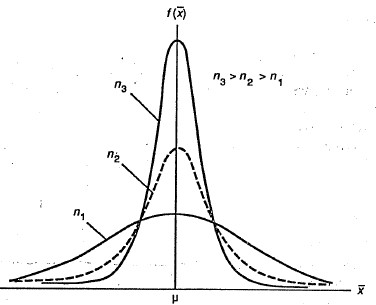
\includegraphics{pics/convergence.jpg}
    \caption{Convergence in probability of the sample mean}
    \label{fig:enter-label8}
\end{figure}

\begin{definition}
    \textbf{Convergence in mean(r)} The sequence of random variables \(X_n\) is said to \textbf{converge in mean of order (r) to X} \(r \geq 1\), and designated \(X_n \stackrel{r}{\longrightarrow} X \text{ if } E[|X_n-X|^r] \text{ exists and } \lim_{n \rightarrow \infty} E[|X_n-X|^r]=0\), that is, if the rth moment of the difference tends to zero. The most commonly used version is \textbf{mean-squared convergence}, which is when r=2. Thus \(X_n \stackrel{m.s.}{\longrightarrow} X\).
\end{definition}

\begin{definition}
    \textbf{Almost sure convergence.} The sequence of random variables \(X_n\) is said to \textbf{converge almost surely} to the real number $x$, and is written as \(X_n \stackrel{a.s.}{\longrightarrow} x\), if \(P[lim X_n=X]=1\). In other words, the sequence \(X_n\) may not converge everywhere to \(x\), but the points where it does not converge form a set of measure zero in the probability sense. More formally, given \(\varepsilon,\delta>0\), there exists \(N\) such that
    \begin{equation*}
        P[|X_{N+1}-x|<\varepsilon,|X_{N+2}-x|<\varepsilon,\dots] > 1-\delta
    \end{equation*}
    that is, the probability of these events jointly occurring can be made arbitrarily close to 1.
\end{definition}

\subsection{Relationships among modes of convergence}

\begin{theorem}
    If \(X_n \stackrel{d} \longrightarrow X \text{ and } Y_n \stackrel{p} \longrightarrow x (\neq 0) \), where $c$ is a constant, 
    \begin{itemize}
        \item[(a)] \((X_n+Y_n) \stackrel{d} \longrightarrow (X+c) \)
        \item[(b)] \((X_n/Y_n) \stackrel{d} \longrightarrow (X/c)\) 
    \end{itemize}
\end{theorem}

\textbf{Proof:} Let \(a-c\) be a continuity point of \(F_X(x)\). The event \(Z_n=(X_n+Y_n) \leq a\) can be expressed as the union of the disjoint events:
\begin{equation*}
    \begin{split}
        S_1: X_n+Y_n \leq a \text{ and } |Y_n-c| \leq \varepsilon\\
        S_1: X_n+Y_n \leq a \text{ and } |Y_n-c| > \varepsilon
    \end{split}
\end{equation*}

Hence \(F_{Z_n}(a)=P(X_n+Y_n \leq a)=P(S_1)+P(S_2)\).\\


\textit{Step 1:} To prove that \(\lim_{n \rightarrow \infty} F_{Z_n}(a) \leq F_{X}(a-c+\varepsilon)\).\\

Define \(S_3:|Y_n-c|> \varepsilon\)\\

Since \(Y_n \stackrel{p} \longrightarrow c\), we have \(P(S_3)\rightarrow 0\). Also, \(S_2 \subset S_3\), which implies that \(P(S_2) \leq P(S_3)\). Because the latter tends to zero, \(P(S_2)\) also tends to zero. Hence
\begin{equation*}
    \lim_{n \rightarrow \infty} F_{Z_n} (a)=\lim_{n \rightarrow \infty} P(S_1)
\end{equation*}

Define \(S_4:(X_n+Y_n) \leq a \text{ and } Y_n>c-\varepsilon\).\\

\(S_4\) implies that \(X_n \leq a-c+\varepsilon\). Therefore
\begin{equation*}
    P(S_4)\leq P(X_n \leq a-c+\varepsilon)=F_X(a-c+\varepsilon)
\end{equation*}

Because \(S_1 \subset S_4\), it follows that
\begin{equation*}
    P(S_1) \leq P(S_4) \leq F_{X_n} (a-c+\varepsilon)
\end{equation*}

Taking the limit as \(n \rightarrow \infty\), we establish Step 1. \\

\textit{Step 2} To prove that \(F_X(a-c-\varepsilon) \leq \lim_{n \rightarrow \infty} F_{Z_n}(a)\).

\begin{equation*}
    P(X_n \leq a-c-\varepsilon)=P(X_n \leq a-c-\varepsilon,|Y_n-c|>\varepsilon)+P(X_n \leq a-c-\varepsilon,|Y_n-c|\leq \varepsilon)
\end{equation*}

As before, the first term \(\leq P(|Y_n-c|>\varepsilon)\), which tends to 0 as n goes to infinity. The second term \(\leq P(X_n \leq a-c-\varepsilon,Y_n \leq c+\varepsilon) \leq P(X_n+Y_n \leq a)=F_{Z_n}(a)\). Combining them and taking the limit we get
\begin{equation*}
    F_X(a-c-\varepsilon)=\lim_{n \rightarrow \infty} P(X_n \leq a-c-\varepsilon) \leq \lim_{n \rightarrow \infty} F_{Z_n}(a)
\end{equation*}

This establishes Step 2. Putting the two steps together we get
\begin{equation*}
    F_X(a-c-\varepsilon) \leq \lim_{n \rightarrow \infty} F_{Z_n}(a) \leq F_X(a-c+\varepsilon)
\end{equation*}

Letting \(\varepsilon \rightarrow 0\), because \(a-c\) is a continuity point of \(F_X(x)\), we get \(F_{Z_n}(a) \rightarrow F_X(a-c)\) as \(n \rightarrow \infty\). But \(F_X(a-c)\) is the distribution function of \(X+c\), that is,
\begin{equation*}
    F_{X+c}(a)=P(X+c\leq a)=P(X \leq a-c)=F_X(a-c)
\end{equation*}

Therefore, \((X_n+Y_n) \stackrel{d} \longrightarrow (X+c)\)   

\begin{theorem}
    If \(X_n \stackrel{p} \longrightarrow X \text{ and } Y_n \stackrel{p} \longrightarrow Y\), then \begin{itemize}
        \item[(a)] \((X_n+Y_n) \stackrel{p} \longrightarrow (X+Y)\)
        \item[(b)] \((X_nY_n)\stackrel{p} \longrightarrow (XY)\)
        \item[(c)] if \(Y_n \text{ and } Y \neq 0\), then \((X_n/Y_n) \stackrel{p} \longrightarrow X/Y\)
    \end{itemize}
\end{theorem}

\begin{theorem}
    If \(g(.)\) is a continuous function, then \(X_n \stackrel{p} \longrightarrow X\) implies that \(g(X_n) \stackrel{p} \longrightarrow g(X)\). In other words, convergence in probability is preserved under continuous transformations.
\end{theorem}

\textbf{Proof:} By the continuity of \(g(.)\) we have, for given \(\varepsilon \text{ and } \delta>0\),
\begin{equation*}
    |X_n-X|<\delta => |g(X_n)-g(X)|<\varepsilon
\end{equation*}

Therefore
\begin{equation*}
    P[|X_n-X|<\delta] \leq P[|g(X_n)-g(X)|<\varepsilon]
\end{equation*}

Because the left-hand side converges to 1, so does the right hand side.

\begin{theorem}
    Convergence in probability implies convergence in distribution, that is, \(X_n \stackrel{p} \longrightarrow X => X_n \stackrel{d} \longrightarrow X\), but the converse need not be true.
\end{theorem}

\textbf{Proof:} By definition, \(X_n \stackrel{p} \longrightarrow X => P[|X_n-X|>\varepsilon]\rightarrow 0 \text{ as } n \rightarrow \infty\). Let \(Y_n=X_n-X\). Then \(\lim_{n \rightarrow \infty} P[|Y_n|>\varepsilon]=0\). This implies that \(Y_n \stackrel{p} \longrightarrow 0\). Also, \(X_n=Y_n+X\). Hence, by Theorem 6.1.
\begin{equation*}
    X_n \stackrel{d} \longrightarrow (0+X)=X
\end{equation*}

That the converse need not be true is illustrated with a simple example. Let \(X_n\) be a sequence of iid random variables with CDF \(F_X(x)\). Then \(X_n \stackrel{d} \longrightarrow X\) trivially. But we cannot state whether \(X_n\) converges in probability or of order (r) to anything.

More specific example: the sample space is \(S=[0,1]\) and \(X_n\) is a sequence of random variables defined as follows:

\begin{equation*}
    X_n(s)=\left\{
    \begin{array}{ll}
        1 & 0 \leq s \leq 1/2 \\
        0 &1/2<s\leq 1
    \end{array}
\right.
\end{equation*}
with a probability of one-half for each. The corresponding sequence of distribution functions is
\begin{equation*}
    F_{X_n}(s)=\left\{
    \begin{array}{ll}
        0 & s<0 \\
        1/2 & 0 \leq s \leq 1/2 \\
        1 & s>1/2
    \end{array}
\right.
\end{equation*}

\begin{figure} [H]
    \centering
    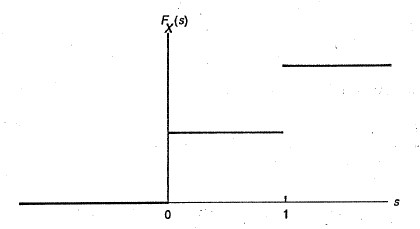
\includegraphics{pics/CDF of random variables.jpg}
    \caption{CDF for the specified sequence of random variables}
    \label{fig:enter-label289}
\end{figure}

Next suppose the random variable \(X\) is defined as

\begin{equation*}
    X(s)=\left\{
    \begin{array}{ll}
        0 & 0 \leq s \leq 1/2 \\
        1 & 1/2 < s \leq 1 \\
    \end{array}
\right.
\end{equation*}

with a probability of one-half for each case. It is easily verified that the corresponding CDF is the same as that for \(X_n\), which means that \(X_n \stackrel{d} \longrightarrow X\) trivially. However, \(X_n-X\) is always equal to 1 and hence \(X_n\) doesn't converge in probability to \(X\).

\begin{theorem}
    Convergence in mean of order r implies convergence in mean of an order less than r, that is, \(X_n \stackrel{r} \longrightarrow X => X_n \stackrel{s} \longrightarrow X (r>s)\), but the converse need not be true.
\end{theorem}

\textbf{Proof:} Because \([E(|Z|^r)]^{1/r}\) is a nondecreasing function of \(r\), we have for \(r>s\)
\begin{equation*}
    E(|X_n-X|^s) \leq E(|X_n-X|^r)
\end{equation*}

It is readily apparent that if the right-hand side of the inequality goes to zero as \(n \rightarrow \infty\), then so does the left-hand side, thus establishing the theorem.

The converse need not be true because even if \(X_n \stackrel{s} \longrightarrow X\), there is no assurance that higher order moments exist.

\begin{theorem}
    Convergence in mean of order \(r \geq 1\) implies convergence in probability, but the converse need not be true.
\end{theorem}

\textbf{Proof:} The proof is trivial and follows directly from Chebyshev's Theorem. Let \(h(X)=|X_n-X|^r\), we see that, for \(\varepsilon>0\),
\begin{equation*}
    P[|X_n-X|>\varepsilon] \leq \frac{E[|X_n-X|^r]}{\varepsilon^r}
\end{equation*}

Because \(X_n \stackrel{r} \longrightarrow X\), the right-hand side has a zero limit. Therefore \(X_n \stackrel{p} \longrightarrow X\).

\begin{theorem}
    Almost sure convergence implies convergence in probability, but the converse need not be true
\end{theorem}

\textbf{Proof:} Let \(A\) be the set \(\{|X_{N+1}-X|<\varepsilon, |X_{N+2}-X|<\varepsilon, \dots \}\) and \(B_i\) be the set \(\{|X_{N+i}-X|<\varepsilon\} \text{ , for } i=1,2,\dots\). Because \(A \subset B_i, P(A) \leq P(B_i) \text{ for } i=1,2,\dots\). If \(X_n\) converges almost surely to $X$, then \(P(A)>1-\delta\), and hence \(P(B_i)>1-\delta\) for \(i=1,2,\dots\), thus implying that \(X_n\) converges in probability also to \(X\).

\textbf{Almost sure convergence is the strongest form of convergence.}

\begin{theorem}

    \begin{itemize}
        \item[(1)] \(X_n \stackrel{a.s.} \longrightarrow x\) if and only if \(P[\sup_{j=n}^{\infty} |X_j-X| > \varepsilon] \rightarrow 0\) as \(n \rightarrow \infty\) for any \(\varepsilon>0\).
        \item[(2)] If \(\sum_{i=1}^{\infty}P(|X_n-X|>\varepsilon)\) is finite for each \(\varepsilon>0\), then \(X_n \stackrel{a.s.} \longrightarrow X\).
        \item[(3)] If \(\sum_{i=1}^{\infty}E[|X_n-X|^r]\) is finite for some $r>0$, then \(X_n \stackrel{a.s.} \longrightarrow X\).
        \item[(4)] If the function \(g(.)\) is continuous at \(X\) and \(X_n \stackrel{a.s.} \longrightarrow X \text{, then } g(X_n) \stackrel{a.s.} \longrightarrow g(X) \)
    \end{itemize}
\end{theorem}

\begin{figure} [H]
    \centering
    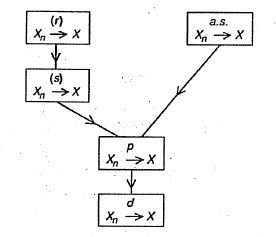
\includegraphics{pics/modes of convergence.jpg}
    \caption{Relationships among modes of convergence}
    \label{fig:enter-label111}
\end{figure}

\subsection{The Weak Law of Large Numbers}

\begin{theorem}
    \textbf{(Khinchin's theorem)}\\
    Let \(\{X_n, n\geq 1\}\) be a sequence of iid random variables with finite mean \(\mu\), and let \(\overline{X}_n=(\sum_{i=1}^{i=n}X_i)/n\). Then
    \begin{equation*}
        \lim_{n\rightarrow \infty} P[|\overline{X}_n-\mu|>\varepsilon]=0
    \end{equation*}
    or equivalently,
    \begin{equation*}
        \lim_{n\rightarrow \infty} P[|\overline{X}_n-\mu|\leq\varepsilon]=1
    \end{equation*}
    In other words, \(plim \overline{X}_n=\mu\)
\end{theorem}

\textbf{Proof:} Expand the characteristic function \(\phi_{X_i}(t)\) around the origin, using the Taylor series
\begin{equation*}
\phi_{X_i}(t)=1+\phi'(0)t+R(t)
\end{equation*}
where \(R(t)\) is a remainder that goes to zero as $t$ goes to zero. But \(\phi'(0)=i\mu\). Therefore \(\phi_{X_i}(t)=1+i\mu t+R(t)\). The characteristic function of \(X_i/n\) is \(1+(i\mu t/n)+R(t/n)\) and hence that of \(\overline{X}_n\) is
\begin{equation*}
    \phi_{\overline{X}_n}(t)=\left[1+\frac{i\mu t}{n} + R(t/n)\right]^n
\end{equation*}
Using the following Lemma, it is readily seen that \(\lim_{n \rightarrow \infty} \phi_{\overline{X}_n}(t)=e^{i\mu t}\), which is the characteristic function of a random variable with all its density at \(\mu\).

\begin{lemma}
    Let \(b(x)\) be a function such that \(\lim_{x \rightarrow 0} b(x)/x=0\). Then
    \begin{equation*}
        \lim_{x \rightarrow 0} [1+ax+b(x)]^{1/x} = e^a
    \end{equation*}
\end{lemma}

\textbf{Proof:} Let \(y=ax+b(x)=x[a+c(x)]\), where \(c(x)\) is a function that converges to \(0\) as x tends to zero. Then
\begin{equation*}
    [1+ax+b(x)]^{1/x}=[(1+y)^{1/y}]^{a+c(x)}=(1+y)^{a/y}[(1+y)^{1/y}]^{c(x)}
\end{equation*}
As \(x \rightarrow 0 \text{ then } y \rightarrow 0\) and the first term becomes \(e^a\). The exponent \(c(x)\) of the second term goes to zero and hence it becomes 1. Hence the limit is \(e^a\).

WLLN can be established even if we relax the assumption that the elements of the sequence \(\{X_n\}\) are identically distributed, provided an alternative condition holds.

\begin{theorem}
     \textbf{(Chebyshev's theorem)}\\
     Let \(\{X_n\}\) be a sequence of independent random variables with means \(\mu_n\) and variances \(\sigma_n^2\), and let \(\overline{\mu}_n=(\sum \mu_i)/n\). If the variances are bounded above, that is, \(\sigma_n^2<c<\infty\), then \((\overline{X}_n-\overline{\mu}_n) \stackrel{p} \longrightarrow 0\).
\end{theorem}

\textbf{Proof:} \(Var(\overline{X}_n)=1/(n^2)\sum \sigma_i^2 \leq c/n\). By Chevyshev's inequality,
\begin{equation*}
    P[|\overline{X}_n-\overline{\mu}_n|\geq \varepsilon] \leq \frac{Var(\overline{X}_n)}{\varepsilon^2} \leq \frac{c}{n \varepsilon^2}
\end{equation*}

Because the right-hand side of the inequality converges to zero, so does the left-hand side. 

When dealing with a sequence of observations over time, the independence assumption is questionable. WLLN will still hold, however, provided \(Var(\overline{X}_n)\) tends to zero as $n$ tends to infinity.

\begin{theorem}
    \textbf{(Markov's theorem)}\\
    Let \(\{X_n\}\) be a sequence of random variables with means \(\mu_n\), and let \(\overline{X}_n\) and \(\overline{\mu}_n\) be as defined in the previous two theorems. If \(Var(\overline{X}_n) \rightarrow 0 \text{ as } n \rightarrow \infty\), then \((\overline{X}_n-\overline{\mu}_n) \stackrel{p} \longrightarrow 0\).
\end{theorem}

\textbf{Proof:} By Chebyshev's inequality,
\begin{equation*}
    P[|\overline{X}_n-\overline{\mu}_n| \geq \varepsilon] \leq \frac{Var(\overline{X}_n}{\varepsilon^2}
\end{equation*}

Because the right-hand side converges to zero, by assumption, so does the left-hand side, thus implying the required convergence in probability.

The three previous theorems specify conditions that are only sufficient but not necessary. Kolmogorov derived the necessary and sufficient condition for the WLLN to hold \textit{without any assumption about independence or identical distribution}.

\begin{theorem}
    \textbf{(Kolmogorov's theorem on WLLN)}\\
    Given the definitions of \(\overline{X}_n \text{ and } \overline{\mu}_n\) in the previous theorems, let \(Z_n=\overline{X}_n-\overline{\mu}_n\). A necessary and sufficient condition for the WLLN to hold, that is, for \(Z_n \stackrel{p} \longrightarrow 0\), is that \(\lim_{n \rightarrow \infty} E[Z_n^2/(1+Z_n^2)]=0\).
\end{theorem}

\textbf{Proof:} Let \(F_n(z)\) denote the distribution function of \(Z_n\). To prove sufficiency, first note that
\begin{equation*}
    P[|Z_n| \geq \varepsilon] = \int_{|z| \geq \varepsilon} dF_n(z)
\end{equation*}
\(|z| \geq \varepsilon\) implies that
\begin{equation*}
    \frac{z^2}{1+z^2} \geq \frac{\varepsilon^2}{1+\varepsilon^2}
\end{equation*}
from which it follows that
\begin{equation*}
    \begin{split}
        P[|Z_n| \geq \varepsilon] = \int_{|z| \geq \varepsilon} dF_n(z) \leq \frac{\varepsilon^2}{1+\varepsilon^2} \int_{|z| \geq \varepsilon} \frac{z^2}{1+z^2} dF_n(z) \\
        \leq \frac{1+\varepsilon^2}{\varepsilon^2} \int \frac{z^2}{1+z^2} dF_n(z) = \frac{1+\varepsilon^2}{\varepsilon^2}E\left[\frac{Z_n^2}{1+Z_n^2}\right]
    \end{split}
\end{equation*}

The condition that the expected value of the expression in the square brackets converges to zero as $n$ goes to infinity is therefore sufficient to establish the theorem. For necessity, note that
\begin{equation*}
    \begin{split}
        P[|Z_n| \geq \varepsilon] = \int_{|z| \geq \varepsilon} dF_n(z) \geq \int_{|z| \geq \varepsilon} \frac{z^2}{1+z^2} dF_n(z) \\
        = \int \frac{z^2}{1+z^2} dF_n(z)-\int_{|z|<\varepsilon} \frac{z^2}{1+z^2} dF_n(z)
    \end{split}
\end{equation*}

Because the first integral is \(E[Z_n^2/(1+Z_n^2)]\) and the second integral is less than \(\varepsilon^2\), we have
\begin{equation*}
    P[|Z_n| \geq \varepsilon] \geq E[Z_n^2/(1+Z_n^2)]-\varepsilon^2
\end{equation*}
Therefore
\begin{equation*}
    0 \leq E \left[\frac{Z_n^2}{1+Z_n^2}\right] \leq \varepsilon^2+P[|Z_n| \geq \varepsilon]
\end{equation*}

Finally, letting \(n \rightarrow \infty\) and \(\varepsilon \rightarrow 0\), the necessity condition is established.

\subsection{The Strong Law of Large Numbers}

The WLLN stated that under certain conditions the sample mean converges in probability to the population mean. We can derive a stronger result: that the sample mean converges almost surely to the population mean. This is the \textbf{strong law of large numbers (SLLN)}. 

Let \(X_1,x_2,\dots,X_n\) be a sequence of random variables with \(E(X_i)=\mu_i<\infty\) and \(\overline{X}_n=(\sum X_n)/n\), and \(\overline{\mu}_n=(\sum \mu_i)/n\).Then, we can show that \((\overline{X}_n-\overline{\mu}_n) \stackrel{a.s} \longrightarrow 0\).

\begin{theorem}
    If the \(X_i\)'s are iid, then \((\overline{X}_n-\overline{\mu}_n) \stackrel{a.s.} \longrightarrow 0\).
\end{theorem}

It follows from this theorem that for \((\overline{X}_n-\overline{\mu}_n)\) to converge in probability to zero but not almost surely, the sequence \(\{X_n\}\) must be either not independent or not identically distributed.

\begin{theorem}
    \textbf{(Kolmogorov's theorem on SLLN}\\
    If the \(X_i\)'s are independent with finite variances, and if \(\sum_{i=1}^{\infty}Var(X_n)/n^2<\infty\), then \((\overline{X}_n-\overline{\mu}_n) \stackrel{a.s.} \longrightarrow 0\).
\end{theorem}

In the case of an iid sequence of random variables, Kolmogorov derived a necessary and sufficient condition for almost sure convercence of the sample mean.

\begin{theorem}
    If the \(X_i\)'s are iid, then a necessary and sufficient condition for \((\overline{X}_n-\overline{\mu}_n) \stackrel{a.s.} \longrightarrow 0\) is that \(E|X_i-\mu_i|<\infty\) for all $i$.
\end{theorem}

\subsection{The Central Limit Theorem}

The Central Limit Theorem states that, under quite general conditions, \textbf{the mean of a sequence of random variables converges to a normal distribution even though the parent distribution isn't normal}. Thus, even if we don't know the statistical distribution of the population from which the sample is being drawn, by having a large sample we can approximate quite well the distribution of the sample mean by the normal distribution.

\begin{theorem}
    Suppose \(X_n (n \geq 1)\) is a sequence of random variables with CDF \(F_n(x)\) and \(X_n \stackrel{d} \longrightarrow X\) with the CDF \(F_X(x)\). Then for any bounded continuous function \(g(x)\),
    \begin{equation*}
        \lim_{n \rightarrow \infty} \int_{-\infty}^{\infty} g(x) dF_n(x)= \int_{-\infty}^{\infty} g(x) dF(x)
    \end{equation*}
    In the case of continuous random variables, this takes the form of
    \begin{equation*}
        \lim_{n \rightarrow \infty} \int_{-\infty}^{\infty} g(x) f_n(x)= \int_{-\infty}^{\infty} g(x) f(x)
    \end{equation*}
\end{theorem}

Thus we can take the limit inside the integral.

\begin{theorem}
    Suppose \(X_n (n \geq 1)\) is a sequence of random variables with CDF \(F_n(x)\) and \(X_n \stackrel{d} \longrightarrow X\) with the CDF \(F_X(x)\). Let the corresponding characteristic functions be \(\phi_n(t) \text{ and } \phi(t)\). Then \(\lim_{n \rightarrow \infty} \phi_n(t)=\phi(t)\). Conversely, if \(\phi_n(t) \rightarrow \phi(t)\), which is continuous at \(t=0\), then \(\phi(t)\) is a characteristic function and the corresponding distribution functions are such that \(F_n(x) \rightarrow F(x)\).
\end{theorem}

\begin{theorem}
    \textbf{(Central limit theorem)}\\
    Let \(X_1,X_2,\dots,X_n\) be a sequence of random variables, \(S_n\) be their sum \(\sum_{i=1}^{i=n} X_i\), and \(\overline{X}_n\) be their mean \(S_n/n\). Define the standardized mean
    \begin{equation*}
        Z_n=\frac{\overline{X}_n-E(\overline{X}_n)}{\sqrt{Var(\overline{X}_n)}} = \frac{S_n-E(S_n)}{\sqrt{Var(S_n)}}
    \end{equation*}
    Then, under a variety of alternative assumptions, \(Z_n \stackrel{d} \longrightarrow N(0,1)\).
\end{theorem}

\textit{de Moivre's Theorem:} \(X_i\)'s are independent Bernoulli variates.\\

\textit{Lindberg-Levy Theorem:} \(X_i\)'s are independent and identically distributed with \(Var(X_i)=\sigma^2<\infty\).\\

\textit{Liapounov Theorem:} \(X_i\)'s are independent with \(E(X_i)=\mu_i\), \(Var(X_i)=\sigma_i^2\), \(E[|X_i-\mu_i|^{2+\delta}]=\rho_i<\infty (\delta>0),\) and
\begin{equation*}
    \lim_{n \rightarrow \infty} \frac{(\sum_{i=1}^{i=n} \rho_i)^2}{(\sum_{i=1}^{i=n} \sigma_i^2)^{2+\delta}}=0
\end{equation*}\\

\textit{Lindberg-Feller Theorem} \(X_i\)'s are independent, \(E(X_i)=\mu_i\), \(Var(X_i)=\sigma_i^2\), \(s_n^2=\sum_{i=1}^{i=n}\sigma_i^2\), \(S_n=\sum_{i=1}^{i=n}X_i \text{, and for } \varepsilon>0\),
\begin{equation*}
    \lim_{n \rightarrow \infty} \frac{1}{s_n^2} \sum_{i=1}^{n} \left[ \int_{|x-\mu_i|>\varepsilon S_n} (x-\mu_i)^2 dF_i(x) \right]=0
\end{equation*}

\textbf{Proof:} The standardized \(Z_n\) can be written as: \(Z_n=\sum_{i=1}^{i=n}u_i\), where \(u_i=(X_i-\mu)/(\sigma/\sqrt{n})\) are all iid. Because of the iid property, \(\phi_{Z_n}(t)=[\phi_{u_i}(t)]^n\). Let \(\phi(t)\) be the characteristic function of \((X_i-\mu)/\sigma\). Taylor expansion of \(\phi(t)\) gives
\begin{equation*}
    \phi(t)=\phi(0)+\phi'(0)t+\phi''(0)\frac{t^2}{2}+R(t^2)
\end{equation*}

where \(R(.)\) is a remainder that goes to zero as \(t\) goes to zero. We have

\begin{equation*}
    \begin{split}
        \phi(0)=1, \hspace{0.5cm} \phi'(0)=iE[(X_i-\mu_i)/\sigma]=0\\
        \phi''(0)=i^2 Var[(X_i-\mu_i)/\sigma]=-1
    \end{split}
\end{equation*}

Therefore, \(\phi_{u_i}(t)=\phi(t/\sqrt{n})=1-(t^2/2n)+R(t^2/n)\). Hence,
\begin{equation*}
    \phi_{Z_n}(t)=[\phi(t/\sqrt{n})]^n=\left[1-\frac{t^2}{2n}+R(t^2/n) \right]^n
\end{equation*}

By Lemma 6.1, \(\lim_{n \rightarrow \infty} \phi_{Z_n}(t)=e^{-t^2/2}\) which is the characteristic function of the standard normal. By the uniqueness and continuity theorems for characteristic functions, \(Z_n \stackrel{d} \longrightarrow N(0,1)\)

\subsection{Multivariate Central Limit Theorem}

\begin{lemma}
    Let $X$ be a random vector with \(E(X)=\mu\) and covariance matrix \(\Sigma\). If every nontrivial linear combination of the elements of $X$ is normally distributed, then \(X\sim MVN(\mu,\Sigma)\)
\end{lemma}

\textbf{Proof:} Define \(Y=c'X\), where $c$ is any \(k \times 1\) vector of constants. Let the scalar random variable $Y$ have mean $v$ and variance $\sigma^2$. We have
\begin{equation*}
    v=c'\mu \hspace{0.5cm} \text{and} \hspace{0.5cm} \sigma^2=c'\Sigma c
\end{equation*}

By assumption, \(Y \sim N(v,\sigma^2)\) and hence its characteristic function is
\begin{equation*}
    E(e{itc'X})=\exp[itv-1/2 \sigma^2t^2]=\exp[itc'\mu-1/2t^2c'\Sigma c]
\end{equation*}

Define the \(k \times 1\) vector \(s=tc\) and substitute for it in the above equation:

\begin{equation*}
    E(e^{is'X})=\exp[is'\mu-1/2s' \Sigma s]
\end{equation*}

But this can be identified as the characteristic function of the multivariate random variable $X$ with mean vector $\mu$ and covariance matrix $\Sigma$. This establishes the lemma.

\begin{theorem}
Let \(X_n (n \geq 1)\) be a sequence of k-variate random variables, independently and identically distributed with the mean vector $\mu$ and covariance matrix $\Sigma$, and let \(\overline{X}_n=(\sum_{i=1}^{i=n}X_i)/n\). Then
\begin{equation*}
    Z_n=\sqrt{n}(\overline{X}_n-\mu) \stackrel{d} \longrightarrow N_k(0,\Sigma)
\end{equation*}
\end{theorem}

\textbf{Proof:} Consider a \(k \times 1\) vector of constants and the linear combination \(Y_n=c'(X_n-\mu)\). \(Y_n\) is a sequence of iid scalar random variables with mean 0 and variance \(c' \Sigma c\). By the central limit theorem, \(X_n=\sqrt{n}\overline{Y}_n \stackrel{d} \longrightarrow N(0,c'\Sigma c)\). This means that the characteristic function has the property
\begin{equation*}
    \lim_{n \rightarrow \infty} \phi_{W_n}(t)=\exp[-t^2c' \Sigma c/2]
\end{equation*}

The characteristic function of \(Z_n\) is given by
\begin{equation*}
    \phi_{Z_n}(s)=E(e^{is'Z_n}
\end{equation*}

Choosing \(s=tc\) in the above and noting that \(W_n=\sqrt{n} \overline{Y}_n=c'Z_n\), we get
\begin{equation*}
    \phi_{Z_n}(tc)=E(e^{itc'Z_n})=E(e^{itW_n}) \rightarrow \exp[-t^2 c' \Sigma c/2]
\end{equation*}
which is the characteristic function of \(N(0,c'\Sigma c)\). Thus the limit of every linear combination of the \(X_n\)'s is a normal distribution. Therefore by Lemma 6.2, \(Z_n \stackrel{d} \longrightarrow N(0,\Sigma)\).

\section{Estimation}

We assume that the family of density functions \(f(x;\theta)\) is known but that the values of the parameters \(\theta\) are unknown. The first step in estimation is to obtain observations on one or more random variables. The observations are used to construct estimates of $\theta$. The formula for obtaining the estimate of a parameter is referred to as an \textbf{estimator} and the numerical value associated with it is called an estimate.

The problem of estimation is simply one of obtaining a sample of observations on incomes and the deriving estimators for $\mu$ and $\sigma$. 

\subsection{Small Sample Criteria for Estimators}

A function \(g(\theta)\) is called estimable if there exists a statistic \(u(x)\) such that \(E[u(x)]=g(\theta)\).

\subsubsection{Unbiasedness}

An estimator \(\hat{\theta}\) is called an \textbf{unbiased estimator} of \(\theta\) if \(E(\hat{\theta})=\theta \text{, and } E(\hat{\theta})-\theta=b(\theta)\), if it is nonzero, is called the \textbf{bias}. \(\hat{\theta}\) is a random variable because it is a function of random variables. Unbiasedness means that the population mean of the distribution of \(\hat{\theta}\) is \(\theta\).

\subsubsection{Mean Squared Error}

A commonly used measure is \(E[(\hat{\theta}-\theta)^2]\), which is called the \textbf{mean squared error (MSE)}. It is a measure of how close \(\hat{\theta}\) is, on average, to the true \(\theta\). It can also be written as
\begin{equation*}
    MSE=E[(\hat{\theta}-\theta)^2]=E[\hat{\theta}-E(\hat{\theta})+E(\hat{\theta})-\theta]^2
\end{equation*}

\(E(\hat{\theta})-\theta=b(\theta)\) is the bias in \(\hat{\theta}\). Because it's independent of the observations, \(b(\theta)\) is nonrandom. Hence,
\begin{equation*}
    MSE=E[\hat{\theta}-E(\hat{\theta})]^2+b^2(\theta)E[\hat{\theta}-E(\hat{\theta})]=Var(\hat{\theta})+b^2(\theta)
\end{equation*}
because \(E[\hat{\theta}-E(\hat{\theta})]=0\). Therefore, MSE is the sum of the variance and the square of the bias.

If \(\hat{\theta}\) is unbiased, \(b(\theta)=0\), and hence \(MSE=Var(\hat{\theta})\). Thus, in the case of unbiased estimators we can compare the respective variances. The estimator with the smaller variance is "better" because it will be closer to the true $\theta$.

\subsubsection{Relative Efficiency}

Let \(\hat{\theta}_1\) and \(\hat{\theta}_2\) be two alternative estimators of $\theta$. Then the ratio of the respective MSEs, \(E[(\hat{\theta}_1-\theta)^2]/E[(\hat{\theta}_2-\theta)^2]\) is called the \textbf{relative efficiency} of \(\hat{\theta}_1\) with respect to \(\hat{\theta}_2\). If \(\hat{\theta}_1 \text{ and } \hat{\theta}_2\) are both unbiased, this ratio reduces to \(Var(\hat{\theta}_1)/Var(\hat{\theta}_2)\). 

When comparing two unbiased estimates \(\hat{\theta}_1\) and \(\hat{\theta}_2\), then the one with the smaller variance is better because it is "closer" to the true value. If either of them is biased, there might be a trade-off. The MSE is used to decide whether the trade-off is worth-it, lower values indicating greater efficiency.

\subsubsection{UMVU Estimators}

An estimator \(\hat{\theta}\) of \(\theta\) is called a \textbf{uniformly minimum variance unbiased (UMVU) estimator} if \(E(\hat{\theta})=\theta\) and for any other unbiased estimator \(\theta^*\), \(Var(\hat{\theta}) \leq Var(\theta^*)\) for every \(\theta\). Among a class of unbiased estimators, a UMVU has the smallest variance.

\subsubsection{Sufficiency}

If a statistic \(\hat{\theta}\) that summarizes all the information about \(\theta\) can be found, it would be more convenient to work with it rather than with the individual observations. Thus \(\hat{\theta}\) is a sufficient statistic for \(\theta\).

\begin{definition}
    Let \(\hat{\theta}\) be a sample statistic and \(\theta^*\) any other statistic not a function of \(\hat{\theta}\). Let \(f(x;\theta)\) be the density function. \(\hat{\theta}\) is said to be a \textbf{sufficient statistic} for \(\theta\) if and only if the conditional density of \(\theta^*\) given \(\hat{\theta}\) is independent of \(\theta\), for every choice of \(\theta^*\). Equivalently, the conditional density of the sample given \(\hat{\theta}\), that is, \(f(x_1,x_2,\dots,x_n|\hat{\theta})\) is independent of \(\theta\).
\end{definition}

A sufficient statistic thus reduces the information contained in the individual observations to a single statistic. \textit{Sufficient statistics are not unique}; it would be useful to obtain a statistic that provides the maximum reduction.

\subsubsection{Minimal Sufficiency}

\(\hat{\theta}\) is \textbf{minimal sufficient} if, for any other sufficient statistic \(\theta^*\) we can find a function \(h(.)\) so that \(\hat{\theta}=h(\theta^*)\).

\subsubsection{Completeness}

The concept of \textbf{completeness} is relevant to density functions. A family of densities \(f(x;\theta)\) is said to be complete if \(E[h(x)]=0\) implies that \(h(x)=0\) for all \(\theta\), where \(h(x)\) is a continuous function. Thus the only unbiased estimator of 0 is zero. The usefulness of this concept stems from the fact that if \(f(x;\theta)\) is complete, the two functions of \(x\) with the same expectation must be identical because their difference has zero expectation. Thus, if \(f(x;\theta)\) is complete, then \(E[h_1(x)]=E[h_2(x)]\) implies that \(h_1(x)=h_2(x)\).

\subsection{Large Sample Properties of Estimators}

\subsubsection{Asymptotic Unbiasedness}

If an estimator has the property that \(Var(\hat{\theta}_n) \text{ and } \sqrt{n}(\hat{\theta}_n-\theta)\) tend to zero as the sample size increases, then it is said to be \textbf{asymptotically unbiased}. This is a stronger requirement than to say that \(E(\hat{\theta}-\theta)\) tends to zero.

\subsubsection{Consistency}

As the sample size \(n\) increases, \(\hat{\theta}\) must approach the true \(\theta\). Three types of consistency measures can be identified:
\begin{enumerate}
    \item \textbf{Simple Consistency:} Let \(\hat{\theta}_1,\hat{\theta}_2,\dots,\hat{\theta}_n\) be a sequence of estimators of \(\theta\). This sequence is a \textbf{simple consistent estimator of \(\theta\)} is, for every \(\varepsilon>0\),
    \begin{equation*}
        \lim_{n \rightarrow \infty} P(|\hat{\theta}_n-\theta|<\varepsilon)=1 \hspace{0.5cm} \theta \in \Theta
    \end{equation*}
    Thus \(\hat{\theta}_n\) is a simple consistent estimator if \(Plim \hat{\theta}_n=\theta\).
    \item \textbf{Squared-error Consistency:} The sequence \((\hat{\theta}_n)\) is a \textbf{squared-error consistent estimator of \(\theta\)} if \begin{equation*}
        \lim_{n \rightarrow \infty} E[(\hat{\theta}_n-\theta)^2]=0
    \end{equation*}
    \item \textbf{Strong Consistency:} \(\hat{\theta}_n\) is said to be \textbf{strongly consistent} if \(P\left[\lim_{n \rightarrow \infty} \hat{\theta}_n=\theta \right]=1\)
\end{enumerate}

It can be readily recognized that the first is convergence in probability \((\hat{\theta} \stackrel{p} \longrightarrow \theta)\), the second is convergence in mean square \((\hat{\theta}_n \stackrel{m.s.} \longrightarrow \theta)\) and the third is almost sure convergence \((\hat{\theta}_n \stackrel{a.s.} \longrightarrow \theta)\). Hence, simple consistency is weaker than squared error and almost sure consistency. Since \(MSE=Var(\hat{\theta}_n)+b^2_n(\theta)\), squared error consistency implies that bout the bias and variance approach zero. Thus if \(Var(\hat{\theta}_n) \rightarrow 0 \text{ and } b_n \rightarrow 0\)  (or =0)
, then \(Plim \hat{\theta}_n=\theta\).

\textbf{Important: unbiasedness doesn't imply consistency}.

The sample mean \(\overline{x}_n\) from iid observations with \(E(X)=\mu\) has the property that \(E(\overline{x}_n)=\mu\) and \(Var(\overline{x}_n)=\sigma^2/n \rightarrow 0\). Hence \(\overline{x}_n\) is both unbiased and consistent. As stated before, \(s^2=[\sum (x_i-\overline{x})^2]/(n-1)\) has the property that \(E(s^2)=\sigma^2\). Thus \(s^2\) is an unbiased estimator of \(\sigma^2\), but \(\hat{\sigma}^2=[\sum(x_i-\overline{x})^2]/n=(n-1)s^2/n\) is not. However, because of the strong law of large numbers, they are both strongly consistent estimators.
\begin{equation*}
    \frac{1}{n}\sum(x_i-\overline{x})^2=\frac{1}{n} \sum x_i^2-\overline{x}^2
\end{equation*}

By the strong law, \(\overline{x}\) converges almost surely to $\mu$ and \((\sum x_i^2)/n\) converges almost surely to \(E(x_i^2)\). Therefore,
\begin{equation*}
    \hat{\sigma}^2=\frac{1}{n} \sum(x_i-\overline{x})^2 \stackrel{a.s} \longrightarrow E(x_i^2)-\mu^2=\sigma^2
\end{equation*}

Because \(s^2=n\hat{\sigma}^2/(n-1)\), its probability limit is also \(\sigma^2\). Thus both estimators are strongly consistent.

\subsubsection{Asymptotic Efficiency}

Some estimators are good for certain values of \(\theta\) and others are more efficient in some other range. For instance, let \(\hat{\theta}=\theta_0\) be fixed regardless of observations. If \(\theta=\theta_0\) or near, then \(\hat{\theta}\) is a pretty good estimate; but when \(\theta\) is far from \(\theta_0\), it is a very poor estimate. When we deal with consistent estimators, the range of values for \(\theta\) for which one estimate is more efficient than other shrinks as the sample size increases. This suggests a notion of \textbf{asymptotic efficiency}:

\begin{definition}
    Let \(\hat{\theta}_n\) be a consistent estimator of \(\theta\). \(\hat{\theta}_n\) is said to be \textbf{asymptotically efficient} if there's no other consistent estimator \(\theta_n^*\) for which 
    \begin{equation*}
    \limsup_{n \rightarrow \infty} {[E[\hat{\theta}_n-\theta)^2]/E[\theta_n^*-\theta]^2]}>1 \end{equation*} for all \(\theta\) in some open interval.
\end{definition}

\subsubsection{Best Asymptotic Normality}

The sequence of estimators \((\hat{\theta}_n)\) is the \textbf{best asymptotically normal (BAN)} estimator if all the following conditions are satisfied.
\begin{enumerate}
    \item \(\hat{\theta}_n \stackrel{p} \longrightarrow \theta\) for every \(\theta \in \Theta\), that is \(\hat{\theta}_n\) is consistent.
    \item The distribution of \(\sqrt{n}(\hat{\theta}_n-\theta) \stackrel{d} \longrightarrow N[0,\sigma^2(\theta)]\), where \(\sigma^2(\theta)= \lim Var(\hat{\theta}_n)\).
    \item There's no other sequence \((\theta_n^*)\) that satisfies (1) and (2) and is such that \(\sigma^2(\theta)>\sigma^{*2}(\theta)\) for every \(\theta\) in some open interval. \([\sigma^{*2}(\theta)=\lim Var(\theta_n^{*}]\).
\end{enumerate}

\subsection{The Likelihood Function}

Let \(x_1,x_2,\dots,x_n\) be a sample of observations on \(X\). Then the \textbf{likelihood function} of the parameter \(\theta\) is defined as
\begin{equation*}
    L(\theta;x)=f_X(x_1,x_2,\dots,x_n;\theta)
\end{equation*}
where \(f(.)\) is the joint density function of the \(x_i\)'s. In the case of a random sample with iid observations, the likelihood function reduces to
\begin{equation*}
    L(\theta;x)=\prod_{i=1}^{n} f_X(x_i;\theta)
\end{equation*}

In the case of a discrete random variable, the density function gives the probability of observing the values \(x_1,x_2,\dots,x_n\) \textit{given the value of the parameter \(\theta\)}. The likelihood function on the other hand is a function of \(\theta\) \textit{for a given set of observations}. As the object here is to obtain estimates of unknown parameters based on sample observations, the likelihood function is more relevant in the context of estimation.

\begin{theorem}
    \textbf{Factorization theorem}\\
    
    A statistic \(\hat{\theta}_n\) will be sufficient for \(\theta\) if and only if the likelihood function \(L(\theta;x)\) can be factored as
    \begin{equation*}
    L(\theta;x)=h(\hat{\theta},\theta)g(x_1,x_2,\dots,x_n)
    \end{equation*}
    In other words, \(L\) is the product of two functions, one independent of \(\hat{\theta}\) and the other involving only \(\hat{\theta}\) and \(\theta\).
\end{theorem}

\textbf{Proof:} We assume that \(L(\theta;x)=h(\hat{\theta},\theta)g(x)\) and then show that \(f(x|\hat{\theta})\) is independent of \(\theta\).
\begin{equation*}
    f(x|\hat{\theta}=\theta_0)=\frac{P(X=x \text{ and } \hat{\theta}=\theta_0)}{P(\hat{\theta}=\theta_0)}
\end{equation*}

If \(\hat{\theta} \neq \theta_0\), the numerator is zero, otherwise it is equal to \(L(\theta;x)\) because \(\hat{\theta}=\theta_0\) is then a certainty. Thus the numerator is \(h(\theta_0,\theta)g(x)\). The denominator is
\begin{equation*}
\sum_{\hat{\theta}=\theta_0}P(X=x)=\sum_{\hat{\theta}=\theta_0} h(\hat{\theta},\theta)g(x)=h(\hat{\theta},\theta) \sum_{\hat{\theta}=\theta_0} g(x)
\end{equation*}

Therefore \(f(x|\hat{\theta}=\theta_0)\) is the ratio in which \(h(\theta_0,\theta)\) is common and cancels out. The rest is independent of \(\theta\) and hence \(\hat{\theta}\) is a sufficient statistic for \(\theta\).

To prove necessity we assume that \(f(x|\hat{\theta})=c(x;\hat{\theta})\) is independent of \(\theta\). \(P(X=x)=P(X=x \text{ and } \hat{\theta}=\theta_0)\) when \(\hat{\theta}=\theta_0\) and \(0\) otherwise. Hence, from the definition of conditional probability
\begin{equation*}
\begin{split}
    P(X=x \text{ and } \hat{\theta}=\theta_0) = P(X=x|\hat{\theta}=\theta_0) P(\hat{\theta}=\theta_0)\\
    = c(x;\hat{\theta}) P(\hat{\theta}=\theta_0)
\end{split}
\end{equation*}

Thus, \(L(\theta;x)=c(x;\hat{\theta})h(\hat{\theta},\theta)\), which is the desired factorization because \(c(c;\hat{\theta})\) is independent of \(\theta\) and \(h(\hat{\theta},\theta)\) depends on \(x\) only through \(\hat{\theta}\).

The usefulness of sufficient statistics lies in their ability to help us find unbiased estimators that have the lowest variance.

\begin{theorem}
    \textbf{Rao-Blackwell theorem}\\
    
    Let \(x_i, i=1,2,\dots,n\) be a random sample from the distribution of \(X\) with the density function \(f(x;\theta)\) and let the statistic \(\hat{\theta}=\hat{\theta}(x_1,x_2,\dots,x_n)\) be sufficient for \(\theta\). Also let the statistic \(T=T(x_1,x_2,\dots,x_n)\), not a function of \(\hat{\theta}\), be an unbiased estimator of \(u(\theta)\). Denote by \(v(\hat{\theta})\) the conditional expectation of \(T\) given \(\hat{\theta}\). Then
    \begin{enumerate}
        \item \(E[v(\hat{\theta})]=u(\theta)\), that is, \(v(\hat{\theta})\) is also an unbiased estimator of \(u(\theta)\).
        \item \(Var[v(\hat{\theta})] \leq Var(T)\), that is, the newly constructed unbiased estimator of \(u(\theta)\) has a smaller (no larger) variance.
        \item \(v(\hat{\theta})\) is independent of \(\theta\) and hence can be computed from the sample.
    \end{enumerate}
\end{theorem}

Usefulness: our ultimate objective is to get the "best" estimator of \(\theta\). By inspection of the likelihood function, using the factorization criterion, we may get a sufficient statistic \(\hat{\theta}\). The theorem gives us a procedure by which we can get another unbiased estimator with a smaller variance. This process is called \textbf{Rao-Blackwellization}. Thus, this conditioning of a statistic by a sufficient statistic improves the statistic in the sense that the variance is generally reduced.\\

\textbf{Proof:} Denote the joint density of \(T \text{ and } \hat{\theta}\) by \(g(T,\hat{\theta};\theta)\) and the conditional density of \(T\) given \(\hat{\theta}\) by \(P(T|\hat{\theta})\). Because \(\hat{\theta}\) is a sufficient statistic, \(P(T|\hat{\theta})\) is independent of \(\theta\) and therefore \(E(T|\hat{\theta})\), which is \(v(\hat{\theta})\), is also independent of \(\theta\), proving part (3). For part (1), we simply apply the law of iterated expectations \(E(T)=E_{\hat{\theta}}E[T|\hat{\theta}]\). But by assumption, \(E(T)=u(\theta)\) and \(E[T|\hat{\theta}]=v(\hat{\theta})\). Hence \(E_T=v(\hat{\theta})\), that s, \(v(\hat{\theta})\) is unbiased. To prove part (2), we have to recall Theorem 4.6; we have
\begin{equation*}
    Var(T)=E_{\hat{\theta}}[Var(T|\hat{\theta})]+Var[v(\hat{\theta})] \geq Var[v(\hat{\theta})]
\end{equation*}

\begin{theorem}
    Let \(x_i \sim f(x_i;\theta)\) and let \(\hat{\theta}\) be sufficient. Also let the density of \(\hat{\theta}\) be complete. If a function of \(\hat{\theta}\), say \(v(\hat{\theta})\), exists such that \(E[v(\hat{\theta})]=u(\theta)\), then \(v(\hat{\theta})\) is the UMVU estimator of \(u(\theta)\).
\end{theorem}

\textbf{Proof:} Let \(v^*\) be another unbiased estimator of \(\theta\). Then \(E(v^*)=u(\theta)=E(v)\), that is, \(E[v-v^*]=0\). But since the density of \(\hat{\theta}\), \(E[v-v^*]=0\) implies that \(v-v^*=0\), that is, \(v=v^*\). Hence \(v(\hat{\theta})\) is unique. The minimum variance follows from part (2) of theorem 7.2.

To summarize, suppose that by using some method, we find an unbiased estimator of $\theta$. We then Rao-Blackwellize it with respect to a sufficient statistic of \(\theta\) and check whether the density of the sufficient statistic is complete. If it is, our search has ended and we have the UMVU estimator of $\theta$.

\subsection{The Principle of Maximum Likelihood}

The observations \(x_1,x_2,\dots,x_n\) come from some underlying DGP. Consider two possible choices for \(\theta\), say \(\theta_1 \text{ and } \theta_2\). The probability of observing the sample \(x_1,x_2,\dots,x_n\) is \(L(\theta_1;x)\) if \(\theta_1\) is true and \(L(\theta_2;x)\) is \(\theta_2\) is true. If \(L(\theta_1;x) > L(\theta_2;x)\), then \(\theta=\theta_1\) gives a higher joint probability of the actual realization, namely, that \(x_1,x_2,\dots,x_n\) was observed. In this case we should choose \(\theta_1\) over \(\theta_2\). This is based on the notion that an event occurs because "it is most likely to happen". The generalization of this idea is the \textbf{principle of maximum likelihood}. It says that among all the possible values \(\theta\) can assume, the one it it \textbf{most likely to assume} is the one that maximizes the likelihood function given by
\begin{equation*}
L(\theta;x_1,x_2,\dots,x_n)=f(x_1,x_2,\dots,x_n;\theta)
\end{equation*}

\begin{definition}
    Let
    \begin{equation*}
        L(\theta;x)=f(x_1,x_2,\dots,x_n;\theta)
    \end{equation*}
    be the likelihood function of the sample. Then if the statistic \(\hat{\theta}=u(x_1,x_2,\dots,x_n)\) maximizes \(L(\theta;x)\) for \(\theta \in \Theta\), then \(\hat{\theta}\) is said to be the \textbf{maximum likelihood estimator (MLE)} of \(\theta\). If \(x_1,x_2,x_3,\dots,x_n\) are iid, then
    \begin{equation*}
        L(\theta;x)=\prod_{i=1}^{n} f(x_i;\theta)
    \end{equation*}
    \end{definition}

Thus the MLE procedure selects the density function from the family \(f(x;\theta)\) that makes the actual realization most probable.

If the likelihood function is differentiable with respect to \(\theta\), the first order condition for maximizing the likelihood function is \(dL/d\theta=0\), if \(\theta\) is the only parameter, if \(\partial L/\partial \theta\) if \(\theta\) is one of several parameters. Because the logarithmic transformation is monotonic, \(\partial L/\partial \theta=0\) if and only if \(\partial(\ln L)/\partial \theta=0\). The log-likelihood is more convenient because, for iid observations,
\begin{equation*}
    \frac{\partial \ln L}{\partial \theta}=0=\sum_{i=1}^n \left[\frac{\partial \ln{f(x_i;\theta)}}{\partial \theta} \right]
\end{equation*}
which is often more convenient to solve.

\textbf{The maximum likelihood method need not give unbiased estimates.}

\subsection{Lower Bounds for Variances of Estimator}

Let \(f(x;\theta)\) be the density function from which a random sample \(x_1,x_2,\dots,x_n\) is drawn. Then \(\ln L=\sum_{i=1}^n \ln{f(x_i;\theta)}\).\\

\title{\textbf{Regularity conditions}}
\begin{enumerate}
    \item \(\theta\) lies in an open interval \(\Theta\) of the real line.
    \item For all \(\theta \in \Theta, \partial L/\partial \theta\) and \(\partial^2 L/\partial \theta^2\) exist and are continuous.
    \item \(\int L(\theta;x)dx\) can be differentiated under the integral sign, that is, \(\int [\partial L(\theta;x)/\partial \theta]dx\) exists.
    \item \(E[{\partial \ln{L}/\partial \theta}^2]\) and \(E[\partial^2 \ln{L}/\partial \theta^2]<\infty\) for all \(\theta \in \Theta\)
    \item \(\int T(x_1,x_2,\dots,x_n) L(\theta;x) dx\) can be differentiated under the integral sign with respect to \(\theta\), that is, \(\int T(x_1,x_2,\dots,x_n) [\partial L(\theta;x)/\partial \theta] dx\) exists.    
\end{enumerate}

\subsubsection{The Score and Information of the Sample}

Define
\begin{equation*}
    S(\theta;x)=\frac{\partial(\ln{L})}{\partial \theta} \left[=\sum_{i=1}^n \frac{\partial \ln{f(x_i;\theta)}}{\partial \theta} \text{ for a random sample} \right]
\end{equation*}

\(S(\theta;x)\) is called the \textbf{score function} of the sample. We know that, for continuous random variables, \(\int L(\theta;x)dx=1\). Differentiate both sides partially with respect to \(\theta\). Then
\begin{equation*}
    0=\int \frac{\partial L}{\partial \theta} dx=\int \frac{1}{L} \frac{\partial L}{\partial \theta} L(\theta;x) dx = \int \frac{\partial \ln{L}}{\partial \theta} L dx=E \left[\frac{\partial \ln{L}}{\partial \theta}\right]
\end{equation*}

Hence,

\begin{equation*}
    E(S)=E \left[\frac{\partial \ln{L}}{\partial \theta} \right]=0
\end{equation*}
that is, the score function has zero expectation. Now differentiate the above integral once more with respect to \(\theta\)
\begin{equation*}
    \begin{split}
        0=\int \frac{\partial \ln{L}}{\partial \theta} \frac{\partial L}{\partial \theta} dx + \int \frac{\partial^2 \ln{L}}{\partial \theta^2} L dx\\
        =\int \left(\frac{\partial \ln{L}}{\partial \theta} \right)^2 L(\theta;x) dx + \int \frac{\partial^2 \ln{L}}{\partial \theta} L dx
    \end{split}
\end{equation*}

Therefore,

\begin{equation*}
    E \left[ \left(\frac{\partial \ln{L}}{\partial \theta} \right)^2 \right] = -E \left[\frac{\partial^2 \ln{L}}{\partial \theta^2} \right] = I(\theta)
\end{equation*}

\(I(\theta)\) is called the \textbf{information (or Fisher information) in the sample}. It follows from this that

\begin{equation*}
    Var(S)=Var \left[\frac{\partial \ln{L}}{\partial \theta} \right] = E \left[ \left( \frac{\partial \ln{L}}{\partial \theta} \right)^2 \right] = I(\theta)
\end{equation*}

Thus the score function has zero mean and variance equal to the information.

\begin{theorem}
    \textbf{Cramer-Rao inequality}\\
    Let \(x_i \sim f(x;\theta)\) and \(T=T(x_1,x_2,\dots,x_n)\) be a statistic such that \(E(T)=u(\theta)\), differentiable on \(\theta\). Also assume the regularity conditions. Let \(u(\theta)-\theta=b(\theta)\), the bias in \(T\). Then
    \begin{equation*}
        Var(T) \geq \frac{[u'(\theta)]^2}{I(\theta)} = \frac{[1+b'(\theta)]^2}{I(\theta)}
    \end{equation*}
    where \(I(\theta)\) is Fisher's information.
\end{theorem}

\textbf{Corollary:} If \(T\) is an unbiased estimator of \(\theta\), then \(Var(T) \geq 1/I(\theta)\).

The above inequality is called the \textbf{Cramer-Rao inequality} and the lower bound for \(Var(T)\) is called the \textbf{Cramer-Rao lower bound (CRLB)}.\\


\textbf{Proof:} For any \(T \text{ and } S, Cov^2(T,S) \leq Var(T) Var(S)\). Let \(T=T(x_1,x_2,\dots,x_n)\) be the statistic given above for which \(E(T)=u(\theta)\) and let \(S=S(\theta;x)\) be the score function. We showed that \(E(S)=0\) and \(Var(S)=I(\theta)\). \(Cov(T,S)=E(ST)\) because \(E(S)=0\). Also,
\begin{equation*}
    u(\theta)=E(T)=\int TL dx
\end{equation*}
Differentiate both sides with respect to $\theta$
\begin{equation*}
    \begin{split}
        u'(\theta)=\int T \frac{\partial L}{\partial \theta} dx = \int T \left( \frac{1}{L} \frac{\partial L}{\partial \theta} \right) L dx\\
        = \int TSL dx = E(TS)= Cov(TS)
    \end{split}
\end{equation*}
Using all these, we get
\begin{equation*}
    [u'(\theta)]^2=Cov^2(T,S) \leq I(\theta) Var(T)
\end{equation*}
Therefore
\begin{equation*}
    Var(T) \geq \frac{[u(\theta)]^2}{I(\theta)}=\frac{[1+b'(\theta)]^2}{I(\theta)}
\end{equation*}
because \(u(\theta)=\theta+b(\theta)\). If \(E(T)=\theta\), then \(b(\theta)=0\) and hence the corollary follows.

\section{Tests of Hypotheses}

\subsection{Basic Concepts in Hypothesis Testing}

Consider a family of distributions represented by the density function \(f(x;\theta), \theta \in \Theta\). The term \textbf{hypothesis} stands for a statement or conjecture regarding the values that \(\theta\) might take. It consists of three steps: (1) formulate two opposing hypotheses, (2) derive a test statistic and identify its sampling distribution, (3) derive a decision rule and choose one of the opposing hypotheses.

\subsubsection{Null and Alternative Hypotheses}

A hypothesis can be thought of as a binary partition of the parameter space \(\Theta\) into two sets, \(\Theta_1 \text{ and } \Theta_0\) such that \(\Theta_0 \cap \Theta_1 = \emptyset \text{ and } \Theta_0 \cup \Theta_1 = \Theta\). The set \(\Theta_0\), which corresponds to the statement of the hypothesis, is called the \textbf{null hypothesis} and \(\Theta_1\) is called the \textbf{alternative hypothesis}.

\subsubsection{Simple and Composite Hypotheses}

If the null hypothesis is of the form \(H_0:\theta=\theta_0\) and the alternative is \(H_1:\theta=\theta_1\), then we have a \textbf{simple hypothesis} and a simple alternative. If either \(H_0 \text{ or } H_1\) specifies a range of values for \(\theta\), then we have a \textbf{composite hypothesis}.
\begin{table}[H]
    \centering
    \begin{tabular}{|c|c|c|c|c|}
    \hline
     - & (a) & (b) & (c) & (d)  \\
     \hline
     \(H_0\) & \(\theta=\theta_0\) & \(\theta=\theta_0\) & \(\theta \leq \theta_0\) & \(\theta \geq \theta_0\) \\
     \hline
     \(H_1\) & \(\theta=\theta_1\) & \(\theta \neq \theta_0\) & \(\theta > \theta_0\) & \(\theta < \theta_0\) \\
     \hline
\end{tabular}
    \label{tab:my_label}
\end{table}

Initially we consider a simple hypothesis and a simple alternative only. In this case the problem reduces to one of choosing between the two density functions \(f(x;\theta_0)\) and \(f(x;\theta_1)\).

\subsubsection{Statistical Test}

A decision rule that selects one of the inferences "accept the null hypothesis" or "reject the null hypothesis" for each foreseeable outcome of an experiment is called a \textbf{statistical test}. A test procedure is described by a sample statistic \(T(x)=T(x_1,x_2,\dots,x_n)\) which is called the test statistic. The range of values of \(T\) for which the test procedure recommends the rejection of a hypothesis is called the \textbf{critical region}, and the range for accepting the hypothesis is called the \textbf{acceptance region}.

\subsubsection{Type I and Type II Errors}
\begin{itemize}
    \item Type I error: rejecting \(H_0\) when it's true
    \item Type II error: accepting \(H_0\) when it's false
\end{itemize}

\subsubsection{Power of a Test}

The probability of rejecting the null hypothesis \(H_0\) based on a test procedure is called the \textbf{power of the test}. This probability depends on the value of the parameter \(\theta\), hence it is a function of \(\theta\) denoted by \(\pi(\theta)\).

\subsubsection{Operating characteristic}

The probability of accepting the null hypothesis is known as the \textbf{operating characteristic} and is represented by \(1-\pi(\theta)\).

\subsubsection{Level of Significance and the Size of a Test}

When \(\theta\) is in \(\Theta_0, \pi(\theta)\) gives the probability of Type I error.This probability, denoted by \(P(I)\), will also depend on $\theta$. The maximum value of \(P(I) \text{ when } \theta \in \Theta_0\) is called the  \textbf{level of significance} of a test, denoted by $\alpha$. It is also known as the \textbf{size of a test}. Thus
\begin{equation*}
    \alpha = \max_{\theta \in \Theta_0} P(I)=\max_{\theta \in \Theta_0} \pi(\theta)
\end{equation*}

The level of significance is hence the largest probability of a Type I error. The probability of a Type II error is often denoted by $\beta(\theta)$. It is readily seen to be \(1-\pi(\theta) \text{ when } \theta \in \Theta_1\). Thus,
\begin{equation*}
    \beta(\theta)=P(II)_{\theta \in \Theta_1}=1-\pi(\theta)
\end{equation*}

Ideally we would want to keep both $P(I)$ and $P(II)$ to the minimum no matter what the value of \(\theta\) is: impossible. An attempt to reduce \(P(I)\) increases \(P(II)\).

Example: if we want to reduce \(P(I)\) in a test such that we reject \(H_0 \text{ if } x > d\), then \(d\) must be larger. But in that case we see that \(P(II)\) goes up. The classical testing procedure resolves this dilemma by choosing an acceptable value for \(\alpha\) and then selecting a decision rule that minimizes \(P(II)\). In other words, given \(\alpha\), among the class of decision rules for which \(P(I) \leq \alpha\), choose the one for which \(P(II)\) is minimized or for which \(\pi(\theta)\) is maximized. Such a test (that maximizes \(\pi(\theta)\) subject to \(P(I) \leq \alpha\)) is a \textbf{most powerful (MP) test}. If the critical region obtain this way is independent of the alternative \(H_1\), then we have a \textbf{uniformly most powerful test (UMP)} 

\subsection{The Neyman-Pearson Fundamental Lemma}

\begin{theorem}
    A test with critical region \(C\) having
    \begin{equation*}
        \begin{array}{ccc}
             \frac{L(\theta_1;x)}{L(\theta_0;x)} & \geq k > 0 & \text{ for } x \text{ in } C  \\
             & < k & \text{ for } x \text{ in } \overline{C}
             \end{array}
    \end{equation*}
    is a most powerful test of \(H_0:\theta=\theta_0\) against \(H_1:\theta=\theta_1\) for some size \(\alpha\). If the value \(k\) and the set \(C\) can be chosen to satisfy \(\int_C L(\theta_0;x) dx = \alpha\) exactly, then \(C\) is most powerful among tests of size \(\alpha\).
\end{theorem}

\textbf{Proof:} Let \(A\) be another critical region region of the same size \(\alpha\). Then
\begin{equation*}
    \int_C L(\theta_0;x)dx=\int_A L(\theta_0;x) dx
\end{equation*}
Denote the complementary sets by \(\overline{A} \text{ and } \overline{C}\). The power function is
\begin{equation*}
    \pi(\theta)=P(x \in C|\theta)= \int_C L(\theta;x) dx
\end{equation*}
To demonstrate that the test is most powerful, we want to show that
\begin{equation*}
    \int_C L(\theta_1;x) dx \geq \int_A L(\theta_1;x) dx
\end{equation*}

We have
 \begin{equation*}
 \begin{split}
     \int_C L(\theta_1;x) dx - \int_A L(\theta_1;x) dx = \int_{C \cap A} L(\theta_1;x) dx + \int_{C \cap \overline{A}} L(\theta_1;x) dx \\
     - \int_{A \cap C} L(\theta_1;x) dx - \int_{A \cap \overline{C}} L(\theta_1;x) dx \\
     = \int_{C \cap \overline{A}} L(\theta_1;x) dx -\int_{A \cap \overline{C}} L(\theta_1;x) dx
\end{split}     
\end{equation*}

In \(C, L(\theta_1;x) \geq k L(\theta_0;x)\) and in \(\overline{C}\) the inequality becomes \(-L(\theta_1;x) > - kL(\theta_0;x)\). Therefore the above difference is greater than
\begin{equation*}
    \int_{C \cap \overline{A}} kL(\theta_0;x)dx-\int_{A \cap \overline{C} } kL(\theta_0;x) dx
\end{equation*}

Adding \(\int_{A \cap C}kL(\theta_0;x) dx \) to both integrals, the difference is greater than
\begin{equation*}
    \int_C kL(\theta_0;x) dx - \int_A kL(\theta_0;x)dx=0
\end{equation*}

Therefore the critical region \(C\) is more (no less) powerful than any other region \(A\) of the same size. 

\subsection{Monotone Likelihood Ratio}

We need a procedure to test composite hypotheses, preferably with a UMP test. For many distributions this is possible using the ratio \(L(\theta_1;x)/L(\theta_0;x)\), called the \textbf{likelihood ratio}.

\begin{definition}
    The statistical model \(f(x;\theta)\) is said to have the \textbf{monotone likelihood ratio (MLR)} form if there exists a real valued function \(u(x_1,x_2,\dots,x_n)\) such that the likelihood ratio \(\lambda = L_1/L_0\) is a non-decreasing function of \(u(x)\) for each choice of \(\theta_0\) and \(\theta_1\) with \(\theta_1 > \theta_0\)
\end{definition}

\begin{theorem}
    For a model with MLR form, obtain \(u^*\) such that the level of significance \(\alpha=P(u>u^*|\theta=\theta_0)\). Then the test: reject \(H_0\) if \(u(x)>u^*\), accept \(H_0\) if \(u(x)<u^*\) and randomizes if \(u(x)=u^*\) is a UMP test of size \(\alpha\) for \(H_0:\theta \leq \theta_0\) against \(H_1:\theta > \theta_0\).
\end{theorem}

\begin{lemma}
    For a model with MLR form, a most powerful test of \(\theta_0\) against \(\theta_1 (>\theta_0)\) has the form: reject the null hypothesis when \(u(x)>u^*\) and accept it when \(u(x)<u^*\) with possible randomization at the critical value $u^*$.
\end{lemma} 

\textbf{Proof:} The NP lemma says that the MP test has the form \(\lambda>k\). If \(\lambda\) is monotonically increasing in \(u\), then the condition \(\lambda>k\) is equivalent to \(u>u^*\).


\begin{lemma}
    For a model with MLR for, the probability \(P[u(x)>u^*|\theta]\) is a nondecreasing function of \(\theta\).    
\end{lemma}

\textbf{Proof:}
Let \(\theta_2>\theta_1\). MLR property implies that as \(\theta\) increases, the distribution of \(u\) shifts to the right, thus increasing \(P(u>u^*)\), which is the area to the right of a given \(u^*\).

\begin{figure} [H]
    \centering
    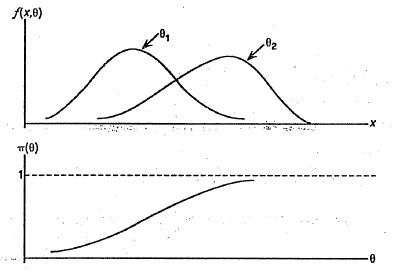
\includegraphics{pics/power function.jpg}
    \caption{Power Function for a model with MLR form}
    \label{fig:enter-label999}
\end{figure}

\textbf{Proof of Theorem 8.2.} By Lemma 8.1, the test is MP for \(\theta=\theta_0\) with the level of significance \(\alpha\). Because of Lemma 8.2., the probability of rejecting \(H_0\) when \(\theta<\theta_0\) is less than or equal to \(\alpha\). Thus the test has size \(\alpha\) for all \(\theta<\theta_0\) and hence is MP for that null hypothesis. Because \(u^*\) is independent of \(\theta_1\), it's also UMP for all alternatives \(\theta_1>\theta_0\).

\subsection{Applications to the Normal Distribution}

\subsubsection{Test on Mean with Known S.D.}

Given \(\sigma=\sigma_0\), the likelihood ratio for \(N(\mu,\sigma_0^2)\) is monotonic in \(\overline{x} \text{ for } \mu_1 > \mu_0\). Therefore the test reject \(H_0: \mu \leq \mu_0 \text{ if } \overline{x}>\mu_0+(\sigma_0 z_\alpha/\sqrt{n})\) is UMP against the alternative \(\mu>\mu_0\). By a similar argument, the test: reject \(H_0\) is \(\overline{x}<\mu_0-(\sigma_0 z_\alpha/\sqrt{n})\) is UMP for \(H_0:\mu \geq \mu_0\) against \(H_1: \mu < \mu_0\).

\subsubsection{Test on S.D with Known Mean}

Let \(\mu=\mu_0\) be known. The log-likelihood ratio is
\begin{equation*}
    \ln \lambda=\ln \left(\frac{L_1}{L_0}\right)=\left[\sum(x_i-\mu_0)^2\right] \left[\frac{\sigma_1^2-\sigma_0^2}{2\sigma_0^2\sigma_1^2} \right] + n \ln \left(\frac{\sigma_0}{\sigma_1} \right)
\end{equation*}

We note that the statistic \(u(x)=\sum(x_i-\mu)^2\) makes this the MLR kind. The critical region for \(H_0:\sigma=\sigma_0, H_1:\sigma=\sigma_1>\sigma_0\), will therefore be \(u>u^*\), where \(u^*\) is obtained so that \(P(u>u^*|\sigma_0)=\alpha\). In order to evaluate \(u^*\), we need the distribution of \(u\) under the null. We know that \([\sum x_i-\mu_0]^2/\sigma_0^2 \sim \chi_n^2\) because it's the sum of squares of $n$ independent normal variates. From this distribution find the point \(u^* \text{ such that } P(\chi_n^2>u^*)=\alpha\). The critical region is \([\sum(x_i-\mu_0)^2]/\sigma_0^2>u^*\). Because $u^*$ is independent of \(\sigma_1\), the test is UMP against all \(\sigma>\sigma_0\). The test for \(\sigma \geq \sigma_0\) against \(\sigma < \sigma_0\) is similar. Find \(u_*\) at the left tail of \(\chi_n^2\). The critical region is now \([\sum(x_i-\mu_0)^2]/\sigma_0^2<u^*\).

\subsubsection{Test on Mean with Unknown S.D.}

We saw that the UMP test for \(H_0: \mu \leq \mu_0\) against \(H_1:\mu>\mu_0\) for a given \(\sigma_0\) is \(\overline{x}
<\mu_0+(\sigma_0 z_\alpha /\sqrt{n})\). But as the critical region depends onf \(\sigma_0\), a UMP for a general normal with unknown \(\sigma\) doesn't exist. In this case, however, an alternative test called an \textbf{unbiased test} is available.

\subsubsection{Test on S.D. with Unknown Mean}

As seen earlier, the likelihood ratio is monotone with respect to \(u(x)=\sum (x_i-\mu)^2\), but because $\mu$ is unknown we cannot construct a UMP test.

\subsection{Unbiased Tests}

So far, we've considered null hypotheses of the form \(\theta \leq \theta_0\) or \(\theta \geq \theta_0\). These are one-sided hypotheses. If we carry out a two sided test such that \(H_0: \theta=\theta_0, H_1: \theta \neq \theta_0\), then we have seen that for a model with the MLR form the critical region \(C_1=\{x:u(x)>u^*\}\) is UMP for \(\theta>\theta_0\). By symmetry, the UMP test against the alternatives \(\theta<\theta_0\) will be \(C_2=\{x:u(x)<u^*\}\). The corresponding power functions are the solid lines in Figure 18. We note that when \(\theta<\theta_0\), the power for the region \(C_1\) is less than \(\alpha\), and similarly for \(C_2\) when the alternative is \(\theta>\theta_0\). If follows that if we use \(C_1\) or \(C_2\) for the two-sided alternative \(\theta \neq \theta_0\), then we have the undesirable property that the probability of rejecting a true hypothesis is larger than the probability of rejecting a false one. Unfortunately, the UMP doesn't exist in this case. We therefore have to restrict our attention to a smaller class of tests: we require that \textbf{the probability of rejection when a hypothesis is false is at least \(\alpha\)}. When the null hypothesis is \(\theta=\theta_0\), this requires that the power function be a minimum at that point. This is called an \textbf{unbiased test}.

\begin{figure} [H]
    \centering
    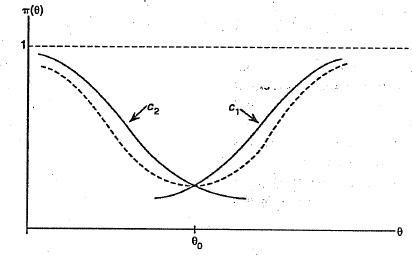
\includegraphics{pics/unbiased.jpg}
    \caption{Illustration of an unbiased test}
    \label{fig:enter-label989}
\end{figure}

\begin{definition}
    A test of \(H_0:\theta \in \Theta_0\) against the alternative \(H_1:\theta \in \Theta_1\) is said to be unbiased if
    \begin{equation*}
        P(I) \leq \alpha \text{ for all } \theta \in \Theta_0 \text{ and } \pi(\theta)\geq \alpha \text{ for all } \theta \in \Theta_1
        \end{equation*}
\end{definition}

\begin{theorem}
    For a one-parameter exponential family of densities, the \textbf{UMP unbiased (UMPU) test} of size \(\alpha\) for \(H_0:\theta=\theta_0,H_1:\theta \neq \theta_0\) is one of the form: reject \(H_0\) is \(u(x)>u_1 \text{ or } u(x)<u_2\), and accept \(H_0 \text{ if } u_1<u(x)<u_2\), with possible randomization at \(u_1 \text{ and } u_2\) in the discrete case. The constants \(u_1 \text{ and } u_2\) are determined by the following conditions:
    \begin{itemize}
        \item The size of the test must be $\alpha$.
        \item Because of unbiasedness, \(\pi(\theta)\) must have a minimum at \(\theta=\theta_0\). If the distribution of \(u(x)\) is symmetric about the origin, an equal tail test with \(u_1=-u_2\) is UMPU.
    \end{itemize}
\end{theorem}


\subsection{UMPU Tests for Multiparameter Exponential Families}

\(\sigma_0\) is generally unknown and is hence a \textbf{nuisance parameter}. UMPU tests do exist on \(\theta\) in the presence of such nuisance parameters provided the density belongs to the exponential family. The trick is to use the conditional distribution of the test statistic given sample estimators for the nuisance parameters.

\begin{definition}
    A density function is said to belong to the \textbf{multiparameter exponentially family} if it can be expressed as
    \begin{equation*}
        f(x;\theta,\lambda)=A(\theta,\lambda) \exp{\left[\theta u(x)+\sum_{j=1}^{k} \lambda_j S_j(x)\right]} H(x)
    \end{equation*}
    where \(\theta\) is the parameter of interest and \(\lambda_1,\lambda_2,\dots,\lambda_k\) are the remaining parameters of the distribution.
\end{definition}

\begin{theorem}
    For a model with the exponential form defined above, the UMPU test of size \(\alpha \text{ for } \theta \leq \theta_0\) against \(\theta <\theta_0\) has the form: reject \(H_0\) if \(u(x)>k(s)\), accept \(H_0 \text{ if } u(x)<k(s)\), with possible randomization when \(u(x)=k(s)\), where $s$ is a set of estimators for \(\lambda\). The critical value \(k(s)\) is chosen so that \(P(u>k(s)|s;\theta=\theta_0)=\alpha\) for each value of $s$.
\end{theorem}

\begin{theorem}
    For the model with the exponential form, the \textbf{(UMPU test} of size \(\alpha\) for \(H_0:\theta=\theta_0,H_1:\theta \neq \theta_0\) is one of the form: reject \(H_0\) is \(u(x)>k_1(s) \text{ or } u(x)<k_2(s)\), and accept \(H_0 \text{ if } k_1(s)<u(x)<k_2(s)\), with possible randomization at \(u=k_1 \text{ and } u=k_2\). The critical values \(k_1 \text{ and } k_2\) are determined so that he size of the test is $\alpha$ and that the power function\(pi(\theta)\) has a minimum at \(\theta=\theta_0\). If the conditional distribution of \(u(x)\) given $s$ is symmetric about the origin, an equal tail test with \(k_1=-k_2\) is UMPU.
    \end{theorem}

\subsection{Generalized Likelihood Ratio Tests}

\begin{definition}
    The \textbf{generalized likelihood ratio} test statistic for testing \(\theta \in \Theta_0\) against \(\theta \in \Theta_1\) is given by
    \begin{equation*}
        \lambda(x)=\frac{\sup_{\theta \in \Theta_0} L(\theta;x)}{\sup_{\theta \in \Theta} L(\theta;x)}
    \end{equation*}
    where \(H_0:\theta \in \Theta_0\) is the null hypothesis and \(\Theta\) is the entire parameter space.
\end{definition}

What we do when constructing this ratio is to maximize the likelihood over the restricted space $\Theta_0$ and also without any restrictions. The denominator of \(\alpha\) corresponds to the maximum likelihood estimator \(\hat{\theta}\). If \(\lambda\) is small, we can suspect that there are parameter values in the alternative hypothesis for which the observed sample is much more likely than for any other parameter value in the null hypothesis. This would suggest that we should reject the null hypothesis in this case. This notion is formulated as the \textbf{likelihood ratio (LR) test}.

\begin{definition}
    The critical region for testing \(H_0:\theta \in \Theta_0\) by a likelihood ratio test is \(0<\lambda<k\), where \(k\) is determined by the condition \(P(0<\lambda<k|\theta \in \Theta_0) \leq \alpha\).
\end{definition}

Although the LR test isn't based on any optimality procedure, it nevertheless gives remarkably reasonable tests that sometimes reduce to tests that are UMP or UMPU.

\begin{theorem}
    Let \(\lambda\) be the likelihood ratio and let \(u(\lambda)\) be a monotonic function of \(\lambda\). Then the LR test based on \(\lambda\) is equivalent to an appropriate test on \(u(\lambda)\). If \(u(\lambda)\) is monotonic increasing, then the critical region is of the form: reject \(H_0 \text{ if } u_1<u(\lambda)<u_2\), where the end points are determined to satisfy the size condition \(\alpha=P(u_1<u<u_2|\theta \in \Theta)\). If \(u(\lambda)\) is monotonic decreasing, then the critical region becomes \(u<u_1\) and \(u>u_2\).
\end{theorem}

\subsection{LR Tests on the Mean and S.D. of a Normal Distribution}

\subsubsection{Test on the Mean with an Unknown S.D.}

We have \(H_0:\mu=\mu_0 \text{ and } H_1: \mu \neq \mu_0\). The first step is to maximize the likelihood with no constraints; the MLEs are \(\hat{\mu}=\overline{x}\) and \(\hat{\sigma}^2=[\sum (x_i-\overline{x})^2]/n\). This gives
\begin{equation*}
    \hat{L}=L(\hat{\theta};x)=\left(\frac{1}{\hat{\sigma}\sqrt{2\pi}}\right)^n e^{-n/2}
\end{equation*}

When \(\mu=\mu_0\), the MLE of \(\sigma\) (call it \(\Tilde{\sigma}\)) is given by \(\Tilde{\sigma}^2=[\sum (x_i-\mu_0)^2]/n\). This gives
\begin{equation*}
    \Tilde{L}=L(\Tilde{\theta};x)=\left(\frac{1}{\Tilde{\sigma}\sqrt{2\pi}}\right)^n e^{-n/2}
\end{equation*}

The likelihood ratio is therefore
\begin{equation*}
    \begin{split}
        \lambda=\frac{\Tilde{L}}{\hat{L}}=\left( \frac{\hat{\sigma}}{\Tilde{\sigma}}\right)^n = \left[\frac{\sum(x_i-\overline{x})^2}{\sum(x_i-\mu_0)^2} \right]^{n/2} = \left[\frac{\sum(x_i-\overline{x})^2}{\sum(x_i-\overline{x}+\overline{x}-\mu_0)^2} \right]^{n/2}\\
        = \left[\frac{\sum(x_i-\overline{x})^2}{\sum(x_i-\overline{x})^2+n(\overline{x}-\mu_0)^2} \right]^{n/2}=\left[\frac{1}{1+\frac{t_c^2}{n-1}} \right]^{n/2} \\
        \text{ where } t_c^2=\frac{(\overline{x}-\mu_0)^2}{s^2/n} \text{ and } s^2=\frac{\sum(x_i-\overline{x})^2}{t-1}
    \end{split}
\end{equation*}

We note that \(\lambda\) is a monotonic decreasing function of \(t_c^2\) and hence the critical region \(\lambda<k\) is equivalent to \(t_c^2>t^{*2}\), where the constant \(t^{*}\) is determined so that \(P(t_c^2>t^{*2})=2P(t_c>t^*)=\alpha\), the level of significance. The null hypothesis is thus rejected if \(t_c<-t^* \text{ or } t_c>t^*\). \(t_c\) has the Student's t distribution with \(n-1\) degrees of freedom.

\subsubsection{Test on the S.D. with an Unknown Mean}

Here \(H_0:\sigma=\sigma_0\) and \(H_1:\sigma \neq \sigma_0\). The likelihood function is
\begin{equation*}
    L=\left(\frac{1}{\sigma \sqrt{2\pi}}\right)^n e^{-\sum(x_i-\mu)^2/(2\sigma^2)}
\end{equation*}

As before, the MLEs are \(\hat{\mu}=\overline{x} \text{ and } \hat{\sigma}^2=[\sum(x_i-\overline{n})^2]/n\). This gives
\begin{equation*}
    \hat{L}=\left(\frac{1}{\hat{\sigma}\sqrt{2\pi}} \right)^n e^{-n/2}
\end{equation*}

Under the null hypothesis \(\sigma=\sigma_0\), the MLE for \(\mu \text{ is } \overline{x}\). The likelihood function is now

\begin{equation*}
    L_0=\left(\frac{1}{\sigma_0\sqrt{2\pi}} \right)^n \exp{\left(\frac{\sum(x_i-\overline{x})^2}{2\sigma_0^2} \right)}=\left(\frac{1}{\sigma_0\sqrt{2\pi}} \right)^n \exp{\left(-\frac{n \hat{\sigma}^2}{2 \sigma_0^2}\right)}
\end{equation*}

The log-likelihood ratio becomes
\begin{equation*}
    \ln{\lambda}=\frac{n}{2} \ln{u}-\frac{nu}{2}+\frac{n}{2}
\end{equation*}

where \(u=\hat{\sigma}^2/\sigma_0^2\). The above function graphs as in Figure 19 with the maximum at \(u=1\). It is readily seen that the critical region \(\lambda<k\) translates into \(u<u_1\) or \(u>u_2\) where the end points are chosen appropriately. $u$ has the $\chi_{n-1}^2$ distribution.

\begin{figure} [H]
    \centering
    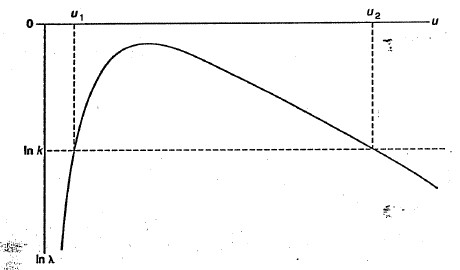
\includegraphics[width=3.5in]{pics/loglikelihood.jpg}
    \caption{Log-likelihood for the variance of a normal population}
    \label{fig:enter-label1099}
\end{figure}

\subsection{The Wald, Likelihood Ratio and Lagrange Multiplier Tests}

In all of these methods two models are formulated: a restricted model and an unrestricted model. The restricted model is imposed by imposing linear or nonlinear constraints on the parameters, and it corresponds to the null hypothesis. The unrestricted model is the alternative.

\subsubsection{Asymptotic Distribution of the Likelihood Ratio}

Although the LR test gives determinate critical regions in many cases, in other situations the distribution of \(\lambda\) or a transformation of it is difficult to obtain. One can obtain the asymptotic distribution of $\lambda$ and use it to obtain the critical region under the null hypothesis.

\begin{theorem}
    Let \(x_1,x_2,\dots,x_n\) be an iid sample of observations form a random variable with density function \(f(x,\theta_1,\theta_2,\dots,\theta_k)\). Suppose we wish to test the null hypothesis \(\theta_1=\theta_1^0,\theta_2=\theta_2^0,\dots,\theta_k=\theta_k^0\). Let $\lambda$ be the likelihood ratio defined as \(L_0/\hat{L}\). Then \(-2\ln{\lambda}\) is asymptotically distributed as \(\chi_k^2\). Thus for large $n, \chi_k^2$ is an approximation to the distribution of \(-2 \ln{\lambda}\).
\end{theorem}

\textbf{Proof:} Let \(H_0:\theta=\theta_0\) be true and let \(\hat{\theta}_n\) be the MLE of \(\theta\). We can expand the log-likelihood in a small neighborhood of \(\theta\) as follows:
\begin{equation*}
    \ln{L(\theta)}=\ln{L(\hat{\theta}_n)}+S'(\hat{\theta}_n)(\theta-\hat{\theta}_n)+\frac{1}{2}(\theta-\hat{\theta}_n)'\left[\frac{\partial S(\theta_n^*)}{\partial \theta}\right] (\theta-\hat{\theta}_n)
\end{equation*}

\(S'\) is the transpose of the score function, \(\partial S/\partial \theta=\partial^2 \ln{L}/\partial \theta \partial \theta'\) and \(|\theta-\theta_n^*| \leq |\theta-\hat{\theta}_n|\). Using the fact that \(S(\hat{\theta}_n)=0\) because \(\hat{\theta}_n\) is MLE, we have
\begin{equation*}
    \ln{L(\theta_0)}-\ln{L(\hat{\theta}_n)}=\frac{1}{2} (\hat{\theta}_n-\theta_0)'\left[\frac{\partial S(\theta_n^*)}{\partial \theta}\right] (\hat{\theta}_n-\theta_0)
\end{equation*}
Hence
\begin{equation*}
    -2 \ln{\lambda} = \sqrt{n} (\hat{\theta}_n-\theta_0)' \left[-\frac{1}{n} \frac{\partial S(\theta_n^*)}{\partial \theta}\right] \sqrt{n} (\hat{\theta}_n-\theta_0)
\end{equation*}

The information matrix is \(I(\theta)=E[-\partial S/\partial \theta]\). Let \(\Sigma(\theta)=\lim\limits_{n \rightarrow \infty} I(\theta)/n\). It was showed earlier that
\begin{equation*}
    \left[-\frac{1}{n} \frac{\partial S(\theta_n^*)}{\partial \theta}\right] \stackrel{p} \longrightarrow \Sigma(\theta_0)
\end{equation*}
and that
\begin{equation*}
    \sqrt{n}(\hat{\theta}_n-\theta_0) \stackrel{d} \longrightarrow N[0,\{\Sigma(\theta_0)^{-1}\}]
\end{equation*}

Therefore the quadratic form corresponding to the above distribution has the \(\chi_k^2\) distribution for large $n$. It thus follows that \(-2\ln{\lambda}\) is asymptotically distributed as \(\chi_k^2\).

\subsubsection{The LR Test Procedure}

Generally only a subset of \(\theta\) may be in the null hypothesis, as for example, \(H_0:\mu=\mu_0\) in a normal \((\mu,\sigma^2)\) population. In this case the test procedure should be modified slightly. Let \(\theta'=(\theta'_1,\theta_2')\) be a partition of \(\theta\) into two sets of parameters, with \(k_1\) parameters and \(k_2\) parameters in the second. For the null hypothesis \(\theta_2=\theta_2^0\), the test procedure is as follows. Let \(\hat{L}(\hat{\theta}_1,\hat{\theta}_2)\) be the maximum likelihood with no restriction on \(\theta\) and let \(\Tilde{L}(\Tilde{\theta}_1,\Tilde{\theta}_2^0)\) be the maximum likelihood under the null. If \(\lambda=\Tilde{L}/\hat{L}\) is the likelihood ratio, then \(\xi_{LR}=-2 \ln{\lambda}\) has the asymptotic \(\chi_{k_2}^2\) distribution. We would reject the null hypothesis if \(\xi_{LR}>\chi_{k_2}^2(\alpha)\), the point on the chi-square distribution with \(k_2\) d.f. such that the area to the right is the level of significance given by $\alpha$.

\subsubsection{The Wald Test Procedure}

The Wald test is based directly on the fact that the maximum likelihood estimator of the parameter \(\theta\) is asymptotically normally distributed. 
\begin{equation*}
    \sqrt{n}(\hat{\theta}-\theta) \stackrel{d} \rightarrow N[0,\{\Sigma(\theta)\}^{-1}]
\end{equation*}
where \(\Sigma(\theta)=\lim_{n \rightarrow \infty} I(\theta)/n\). The corresponding quadratic form has a limiting chi-square distribution. Thus, under \(H_0\),
\begin{equation*}
    \xi_W=(\hat{\theta}-\theta_0)'I(\hat{\theta})(\hat{\theta}-\theta_0) \stackrel{d} \rightarrow \chi_k^2
\end{equation*}

The test criterion is to reject the null hypothesis \(\theta=\theta_0\) if the quadratic form \(\xi_W\) is greater than \(\chi_k^2(\alpha)\), the point on the chi-square distribution with \(k\) d.f. and an area of \(\alpha\) to the right of it. To carry out a test on a subset of \(\theta\), suppose that \(\theta'=(\theta_1',\theta_2')\) and that the null hypothesis is \(\theta_2=\theta_2^0\). First partition the information matrix and its inverse as
\begin{equation*}
    I(\theta) = \begin{bmatrix}
        I_{11} & I_{12} \\
        I_{21} & I_{22}
    \end{bmatrix}
    \hspace{0.5cm}
    \text{ and }
    \hspace{0.5cm}
    [I(\theta)]^{-1} = 
    \begin{bmatrix}
        I^{11} & I^{12} \\
        I^{21} & I^{22}
    \end{bmatrix}
\end{equation*}

Applying the partitioned inverse property, we have
\begin{equation*}
    I^{22}=[I_{22}-I_{21}I_{11}^{-1}I_{12}]^{-1}
\end{equation*}

It follows analogously that
\begin{equation*}
    \sqrt{n}(\hat{\theta}_2-\theta_2^0) \stackrel{d} \longrightarrow N\left[0,\lim_{n \rightarrow \infty} (n I^{22}) \right]
\end{equation*}

The relevant quadratic form is now
\begin{equation*}
    \begin{split}
        \xi_W=(\hat{\theta}_2-\theta_2^0)[I^{22}(\hat{\theta})]^{-1}(\hat{\theta}_2-\theta_2^0)\\
        = (\hat{\theta}_2-\theta_2^0)'[I_{22}(\hat{\theta})-I_{21}(\hat{\theta})\{I_{11}(\hat{\theta})\}^{-1}I_{12}(\hat{\theta})](\hat{\theta}_2-\theta_2^0)
    \end{split}
\end{equation*}
which has the large sample chi-square distribution with \(k_2\) degrees of freedom. The null hypothesis \(\theta_2=\theta_2^0\) will be rejected if \(\xi_W>\chi_{k_2}^2(\alpha)\).

\subsubsection{The Lagrange Multiplier Test Procedure}

The likelihood is maximized subject to the constraint \(\theta_2=\theta_2^0\) and a test statistic constructed from the Lagrange multiplier for the constrained maximization. Here we carry out the test directly for the case of testing a subset of the parameters.

\begin{equation*}
    H=L(\theta_1,\theta_2;x)-l'(\theta_2-\theta_2^0)
\end{equation*}
where $l$ is a \(k_2 \times 1\) vector of Lagrange multipliers. The first order condition for maximization is
\begin{equation*}
    \frac{\partial L}{\partial \theta_1} = 0 \hspace{0.5cm} \text{ and } \hspace{0.5cm} \frac{\partial L}{\partial \theta_2}=l
\end{equation*}
which gives the transpose of the score vector as \(S'=[0 \hspace{0.2cm} l']\). Denote the solution to these equations by \(\Tilde{\theta}\). The test based on $l$ is the same as that based on the score function \(S(\theta;x)\).
\begin{equation*}
    \frac{1}{\sqrt{n}}S(\theta;x) \stackrel{d} \longrightarrow N[0,\Sigma(\theta)]
\end{equation*}
where \(\Sigma(\theta)=\lim\limits_{n \rightarrow \infty} I(\theta)/n\). Therefore a test statistic based on the Lagrange multiplier is given by the corresponding quadratic form
\begin{equation*}
    \xi_{LM}=S(\Tilde{\theta})'[I(\Tilde{\theta})]^{-1}S(\Tilde{\theta})=[0 \hspace{0.2cm} l'] \begin{bmatrix}
        I^{11} & I^{12} \\
        I^{21} & I^{22}
    \end{bmatrix} \begin{bmatrix}
        0\\
        l
    \end{bmatrix} = l'I^{22}(\Tilde{\theta})l
\end{equation*}

The null hypothesis will be rejected if \(\xi_{LM}>\chi_{k_2}^2(\alpha)\).

\subsubsection{A Geometric Comparison of the Tests}

\end{document}
